% !TeX spellcheck = en_GB
\documentclass[
 paper=A4,pagesize=automedia,fontsize=12pt,
 BCOR=15mm,DIV=22,
 twoside,headinclude,footinclude=false,
 fleqn,                     % fleqn = linksbündige Ausrichtung von Formeln
 bibtotocnumbered,          % Literaturverz. im Inhaltsverz. eintragen
 liststotoc,                % Abbildungsverz. im Inhaltsverz. eintragen
 listsleft,                 % Abbildungsverz. an der längsten Nummer ausrichten
 %pointlessnumbers,          % kein Punkt nach Überschriftsnummerierung
 cleardoublepage=empty      % Vakatseiten ohne Paginierung
]{scrbook}
\setlength\parindent{0em}

% Kodierung, Schrift und Sprache auswählen
\usepackage[utf8]{inputenc}
\usepackage[T1]{fontenc}
\usepackage{babel}
% damit man Text aus dem PDF korrekt rauskopieren kann
\usepackage{cmap}
% Layout: Kopf-/Fußzeilen, anderthalbfacher Zeilenabstand
\usepackage{scrpage2} \pagestyle{scrheadings}
                      \clearscrheadfoot
                      \ihead{\headmark}\ohead{\pagemark}
                      \automark[subsection]{section}
                      \setheadsepline{0.5pt}
\usepackage{setspace} \onehalfspacing
\deffootnote{1em}{1em}{\textsuperscript{\thefootnotemark }}
% Grafiken, Tabellen, Mathematikumgebungen
\usepackage{graphicx,xcolor}
\usepackage{tabularx}
\usepackage{amsmath,amsfonts,amssymb}
% Darstellung von Fließumgebungen
\usepackage{flafter,afterpage}
\usepackage[section]{placeins}
\usepackage[margin=8mm,font=small,labelfont=bf,format=plain]{caption}
\usepackage[margin=8mm,font=small,labelfont=bf,format=plain]{subcaption}

\numberwithin{equation}{chapter}
\numberwithin{figure}{chapter}
\numberwithin{table}{chapter}

%%%%%%%%%%%%%%%%%%%%%%%%%%%%%%%%%%%%%%%%%%%%%%%%%%%%%%%%%%%%%%%%%%%%%%%%%%%%%%%%
% Ab hier ist Platz für eigene Ergänzungen (Pakete, Befehle, etc.)

% Dieses Paket liefert den Blindtext, der als Platzhalter in den Beispieldateien steht.
% Das kannst Du also entfernen, wenn Du den Blindtext nicht mehr brauchst.
\usepackage{lipsum}
%\usepackage{ bbold }
\usepackage{physics}
\usepackage{svg}
\usepackage{yfonts}
\usepackage{dsfont}
\begin{document}

\frontmatter


% Titelpageseite
\begin{titlepage}
 \begin{tabularx}{\linewidth}{X}
  
\includegraphics[width=6cm]{TU_Logo_SW} \\\hline\hline

  \vspace{4.5em}

  \begin{singlespace}\begin{center}\bfseries\Huge
  
  Learning quantum work extraction protocols with recurrent neural networks
  
  \end{center}\end{singlespace}

  \vspace{5.5em}

  \begin{singlespace}\begin{center}\large
   Bachelor-Arbeit \\ zur Erlangung des Hochschulgrades \\ 
   Bachelor of Science \\ 
   im Bachelor-Studiengang Physik
  \end{center}\end{singlespace}\medskip

  \begin{center}vorgelegt von\end{center}
  \begin{center}
   {\large Felix Soest} \\ geboren am 16.09.1998 in Düsseldorf
  \end{center}\medskip

  \begin{singlespace}\begin{center}\large
   Institut für Theoretische Physik \\
   Fakultät Physik \\
   Bereich Mathematik und Naturwissenschaften \\
   Technische Universität Dresden \\ 2021
  \end{center}\end{singlespace}
 \end{tabularx}
\end{titlepage}


% Gutachterseite
\thispagestyle{empty}\vspace*{48em}

Eingereicht am 08.~Februar~2021\vspace{1.5em}
\par{\large\begin{tabular}{ll}
 1. Gutachter: & Prof.~Dr.~Walter~Strunz \\
 2. Gutachter: & Prof.~Dr.~Oscar~Dahlsten \\
\end{tabular}}


% Abstractseite
\newpage
\begin{center}\large\bfseries Abstract\end{center}
An interesting question in the field of quantum thermodynamics is how to extract the maximum amount of work from a given system.
We consider a two-state quantum system that is driven by a piecewise constant function, from which work can be extracted.
We show that for this system a policy exists that is able to extract a non-negative work output independent of the excitation.
We investigate the system with respect to randomly sampled drives and find their optimal extraction policies numerically.
Using these pairs as training data we employ recurrent neural networks to predict the optimal transducer policy given a drive sequence.
We find that our approach performs reasonably well, even capable of extracting more than 97 \% of the optimum for certain model parameters.
Additionally, we explore the robustness of the model predictions with respect to noise and the ability of our models to generalise to longer drive sequences.

\vspace{10em}
\begin{center}\large\bfseries Zusammenfassung\end{center}
Eine interessante Frage im Gebiet der Quanten-Thermodynamik ist, wie man die maximale Menge an Arbeit aus einem gegebenen System extrahieren kann.
Wir betrachten ein zwei-Niveau-Quantensystem, welches durch eine stückweise konstante Funktion angetrieben wird und aus dem Arbeit extrahiert werden kann.
Wir zeigen, dass für dieses System eine Strategie existiert, die in der Lage ist, eine nicht-negative Arbeit unabhängig von der Anregung zu extrahieren.
Wir untersuchen das System in Bezug auf zufällig generierte Antriebe und finden deren optimale Extraktionssequenz numerisch.
Unter Verwendung dieser Paare als Trainingsdaten verwenden wir rekurrente neuronale Netze, um die optimale Extraktionsstrate-gie einer gegebenen Antriebssequenz vorherzusagen.
Dieser Ansatz funktioniert recht gut, und ist in der Lage, mehr als 97 \% des Optimums für bestimmte Modellparameter zu extrahieren.
Zusätzlich untersuchen wir die Robustheit der Modellvorhersagen in Bezug auf Rauschen und die Fähigkeit unserer Modelle, auf längere Antriebssequenzen zu generalisieren.
 
 
% Inhaltsverzeichnis
%\cleardoublepage
\tableofcontents



% Hauptteil
\mainmatter

\chapter{Introduction}
% !TeX root = ../BA_main_englisch.tex
% !TeX spellcheck = en_GB
Thermodynamics has been a central field of interest in physics ever since its inception in the 19th century \cite{thomson_2011}.

Due to the increasing availability of data and computing power, machine learning methods have become a standard approach in many fields such as natural language processing \cite{DBLP:journals/corr/VaswaniSPUJGKP17}.
Additionally, these methods are being applied to a broad range of problems in the physical sciences, from statistical physics to quantum computing \cite{Carleo_2019, wise2021using}.

Machine learning has also found use in the field of energy harvesting, concerned with extracting energy from external excitations, e.g. vibrations in human motion \cite{Liu2019}.
In this work we extend this concept to the quantum case.
Work extraction is often modelled as a system coupled to a heat bath, and bounds for the extractable work exist \cite{Egloff_2015}.
We take a different approach, following the framework given in \cite{beyer2020}.
We examine a system that can be driven by an arbitrary excitation, modelled as a time-dependent system Hamiltonian.
The transducer is modelled in a similar fashion and can extract work from the system.
By following a policy of local optimisation of the work output, we show that a lower bound of the extractable work exists for specific initial conditions.
We train neural networks to predict transducer protocols given a drive sequence, considering both the case where the sequence is known beforehand and the one where it is not.

The remainder of this work is structured as follows.
In Chapter \ref{background} we review the collision model framework used in our approach and introduce two machine learning architectures.
In Chapter \ref{lower_bound} we show that for a given drive sequence a lower bound on the expectation value of the extractable work exists.
We investigate the system under consideration in Section \ref{dep_dt} and apply the aforementioned architectures in Sections \ref{n_2_ml} to \ref{work_cost}.
We summarise our findings and provide an outlook in Chapter \ref{outlook}.

We use units where $\hbar = 1$.

\chapter{Background} \label{background}
\section{Collision model dynamics} \label{col_model}
% !TeX spellcheck = en_GB
A standard approach to modelling open quantum systems is the collision model.
The system under consideration interacts with a series of ancilla systems through a unitary transformation on the combined system-ancilla state \cite{Lorenzo_2017}. After a short interaction time $\Delta t$, the ancilla systems are traced out to receive the system state.
This type of interaction will in general lead to entanglement between system and ancilla.
This is undesirable in our setting, the reason for which will become apparent in the next paragraph.
To ensure the ancilla and system states remain pure, we follow the approach used in \cite{beyer2020}:
let $\rho_S$ be the density operator of the system under consideration and $\ket{\psi_A}$ the state of the ancilla system.
Given $\Delta t \ll 1$ the time evolution of $\rho_S$ under $H_{AS}$ acting on the combined system is
\begin{align}\label{coll_eq}
\rho'_S & = \mathrm{Tr}_A \{ e^{-i H_{AS} \Delta t} (\ket{\psi_A} \bra{\psi_A} \otimes \rho_S) e^{i H_{AS} \Delta t} \} & = \rho_S - i \Delta t [\expval{H_{AS}}{\psi_A}, \rho_S] + O(\Delta t^2).
\end{align}

In the continuous limit Eq. (\ref{coll_eq}) leads to von-Neumann dynamics on the system for an infinite stream of qubits initialised in the same state $\ket{\psi_A}$:
\begin{align*}
	\dot{\rho}_S = - i [\expval{H_{AS}}{\psi_A}, \rho_S].
\end{align*}

As each ancilla only interacts once with the system and is traced out afterwards, $\rho_S$ remains pure in the limit of $\Delta t \to 0$.


We use this approach as the implementation for our setting, which consists of three qubits: the drive, system and transducer qubits.
We focus on piece-wise constant (PWC) functions of the drive ($\ket{\psi_D}$) and transducer ($\ket{\psi_T}$) qubits, as it greatly reduces computational complexity.
These are implemented by keeping the stream of ancillas $\ket{\psi_A} = \ket{\psi_D} \otimes \ket{\psi_T}$ constant for time $\Delta \mathrm{T}$ (Figure \ref{collmodel}).
The drive and transducer qubits can be set in N discrete intervals represented by ($\theta_D^n, \phi_D^n$) and ($\theta_T^n, \phi_T^n$) respectively (see Figure \ref{pwc}), the system qubit is initialised in a pure state $\rho_S$.
Here, the necessity for pure ancillas, in this case both drive and transducer qubit, becomes clear, as a mixed drive or transducer state would not be compatible with the PWC approach where we assume the experimenter to be in control of drive and transducer at all times.

In the remainder of this work we use the interaction Hamiltonian on the three qubit Hilbert space
\begin{equation*}
H_{DST} = H_{I} \otimes \mathds{1}_T + \mathds{1}_D \otimes H_{I}, \\
H_{I} = \sigma_{+} \otimes \sigma_{-} + \sigma_{-} \otimes \sigma_{+}.
\end{equation*}
Note that the interaction Hamiltonian itself is constant and the time dependence comes from the change in the stream of ancillas only.
The energy scale of the Hamiltonian is therefore limited and so are the dynamics of the system state $\rho_S$.
The time evolution and work extraction is then calculated as follows, where $\Delta \mathrm{T}$ is time span between qubit switching:
\begin{align}
H_S^n &= \bra{\psi_D^n}\bra{\psi_T^n} H_{DST} \ket{\psi_D^n} \ket{\psi_T^n}, \label{relham}\\
\rho_S &((n+1) \Delta \mathrm{T}) = U_n \ \rho_S(n \Delta \mathrm{T}) \ U^{\dagger}_n, \\
U_n &= e^{-iH_S^n \Delta \mathrm{T}}, \\
W &= - \Sigma_n \Tr{\rho_S(n \Delta \mathrm{T}) \ dH_S^n}, \\
dH_S^n &= \bra{\psi_D^n}\bra{\psi_T^{n+1}} H_{DST} \ket{\psi_D^n} \ket{\psi_T^{n+1}} - \bra{\psi_D^n}\bra{\psi_T^n} H_{DST} \ket{\psi_D^n} \ket{\psi_T^n}.	
\end{align}
Here we use the partial Hamiltonian $H_S^n$ on the system at time step $n \in [1, N - 1]$, as well as corresponding system density matrix $\rho_S(n \Delta \mathrm{T})$.
An advantage of this framework is that the extracted work is available to the experimenter as a quantum observable \cite{beyer2020}.

Using the Bloch sphere representation $\ket{\psi} = \cos(\frac{\theta}{2}) \ket{0} + e^{i \phi} \sin(\frac{\theta}{2})\ket{1}$ to represent drive and transducer qubits reduces Eq. (\ref{relham}) to
\begin{align}
	H_S^n &= \frac{1}{2} \left[\sin(\theta_D^n) e^{i\phi_D^n} + \sin(\theta_T^n) e^{i\phi_T^n}\right] \sigma_{+} + h.c. =  H_{DS} + H_{ST}.
\end{align}

\begin{figure}
	\centering
	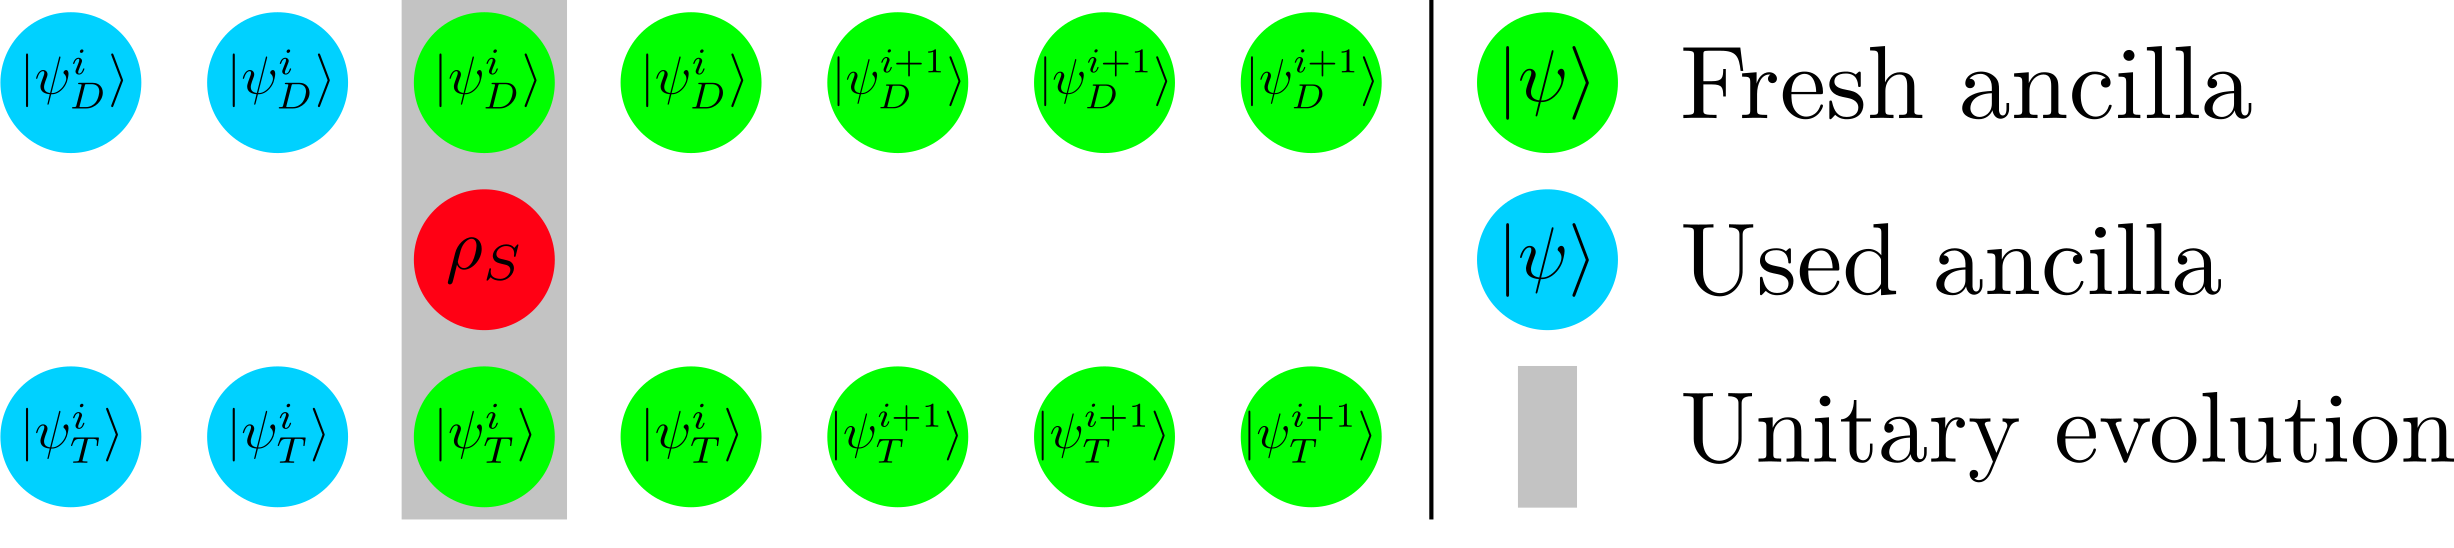
\includegraphics[width=0.85\textwidth]{img/coll2}
	\caption{Collision model used in this work: drive and transducer are series of qubits that interact once with the system and evolve the reduced density operator $\rho_S$. The qubit configuration can be changed in intervals of $\Delta \mathrm{T}$.}
	\label{collmodel}
\end{figure}

\begin{figure}
	\centering
	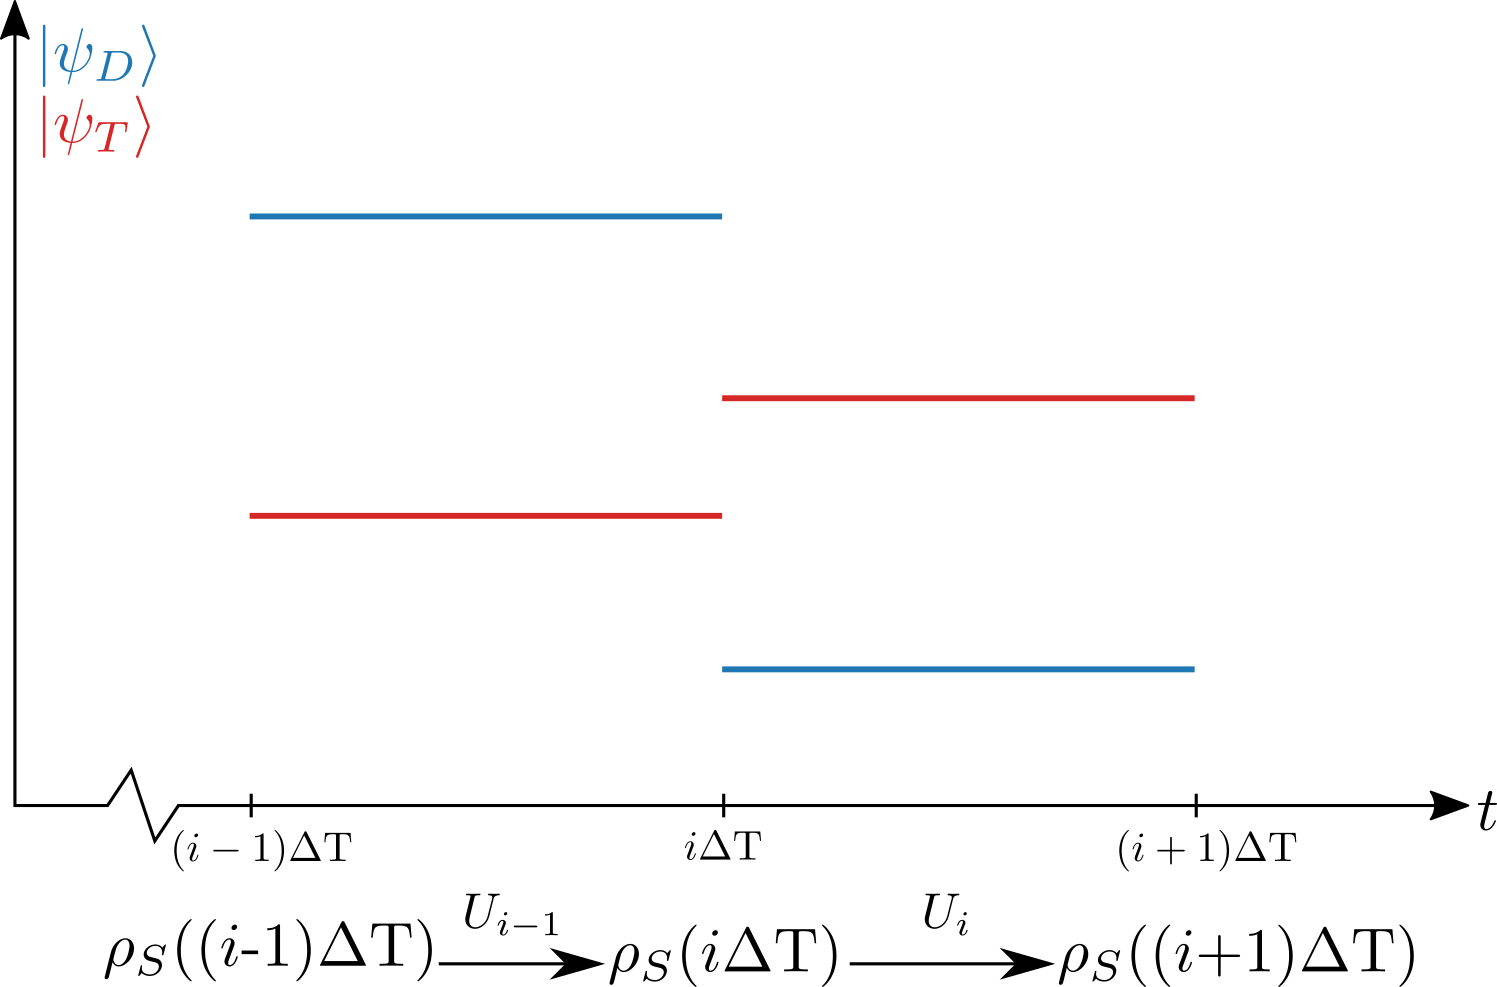
\includegraphics[width=0.6\textwidth]{img/pwc2}
	\caption{Piecewise constant implementation of drive and transducer qubits: the vertical axis represents an arbitrary parameter of the ancilla states. The qubit states are switched instantaneously and then kept constant for $\Delta \mathrm{T}$ while $\rho_S$ evolves unitarily. The piece-wise constant drive and transducer settings lead to a piece-wise constant system Hamiltonian.}
	\label{pwc}
\end{figure}

%\section{Setting}
%Our setting consists of three qubits: the Drive, System and Transducer qubits. The Drive and Transducer qubits can be set by the experimenter in N discrete steps modelled as piecewise constant functions (PWC) of ($\theta_D, \phi_D$) and ($\theta_T, \phi_T$) respectively (see figure \ref{pwc}), the system qubit is initialised in a pure state.
As Drive and Transducer are assumed to be piecewise constant and therefore pure, we model both qubits as ancillary systems introduced in section \ref{col_model} (see figure \ref{collmodel}).

In the remainder of this work we use the interaction Hamiltonian on the three qubit Hilbert space
\begin{equation*}
	H_{DST} = H_{I} \otimes \mathds{1}_T + \mathds{1}_D \otimes H_{I}, \\
	H_{I} = \sigma_{+} \otimes \sigma_{-} + \sigma_{-} \otimes \sigma_{+}
\end{equation*}
unless otherwise noted.
The time evolution and work extraction is then calculated as follows, where $\Delta \mathrm{T}$ is time span between qubit switching\footnote{It is important to make the distinction between $\Delta \mathrm{T}$ and $\Delta t$ introduced in section \ref{col_model}. $\Delta t$ is the collision time of a single qubit while $\Delta \mathrm{T}$ is the time for which the qubits have the same initial state. For each time step $i$ we therefore have $n = \Delta \mathrm{T} / \Delta t$ qubits initialised in the same state.}:
\begin{align}
	H_S^i = \bra{\psi_D^i}\bra{\psi_T^i} H_{DST} \ket{\psi_D^i} \ket{\psi_T^i} \\
	\rho_S^{i+1} = U^i \rho_S^i U^{i\dagger}, \ U^i = e^{-iH_S^i \Delta \mathrm{T}} \\
	W = - \Sigma_i \mathrm{Tr} \ \rho_S^i \ dH_S^i \\
	dH_S^i = \bra{\psi_D^i}\bra{\psi_T^{i+1}} H_{DST} \ket{\psi_D^i} \ket{\psi_T^{i+1}} - \bra{\psi_D^i}\bra{\psi_T^i} H_{DST} \ket{\psi_D^i} \ket{\psi_T^i}.	
\end{align}
Here we use the partial Hamiltonian $H_S^i$ on S at time step $i \in [1, N - 1]$, as well as corresponding system density matrix $\rho_S^i$.


\begin{figure}
	\centering
	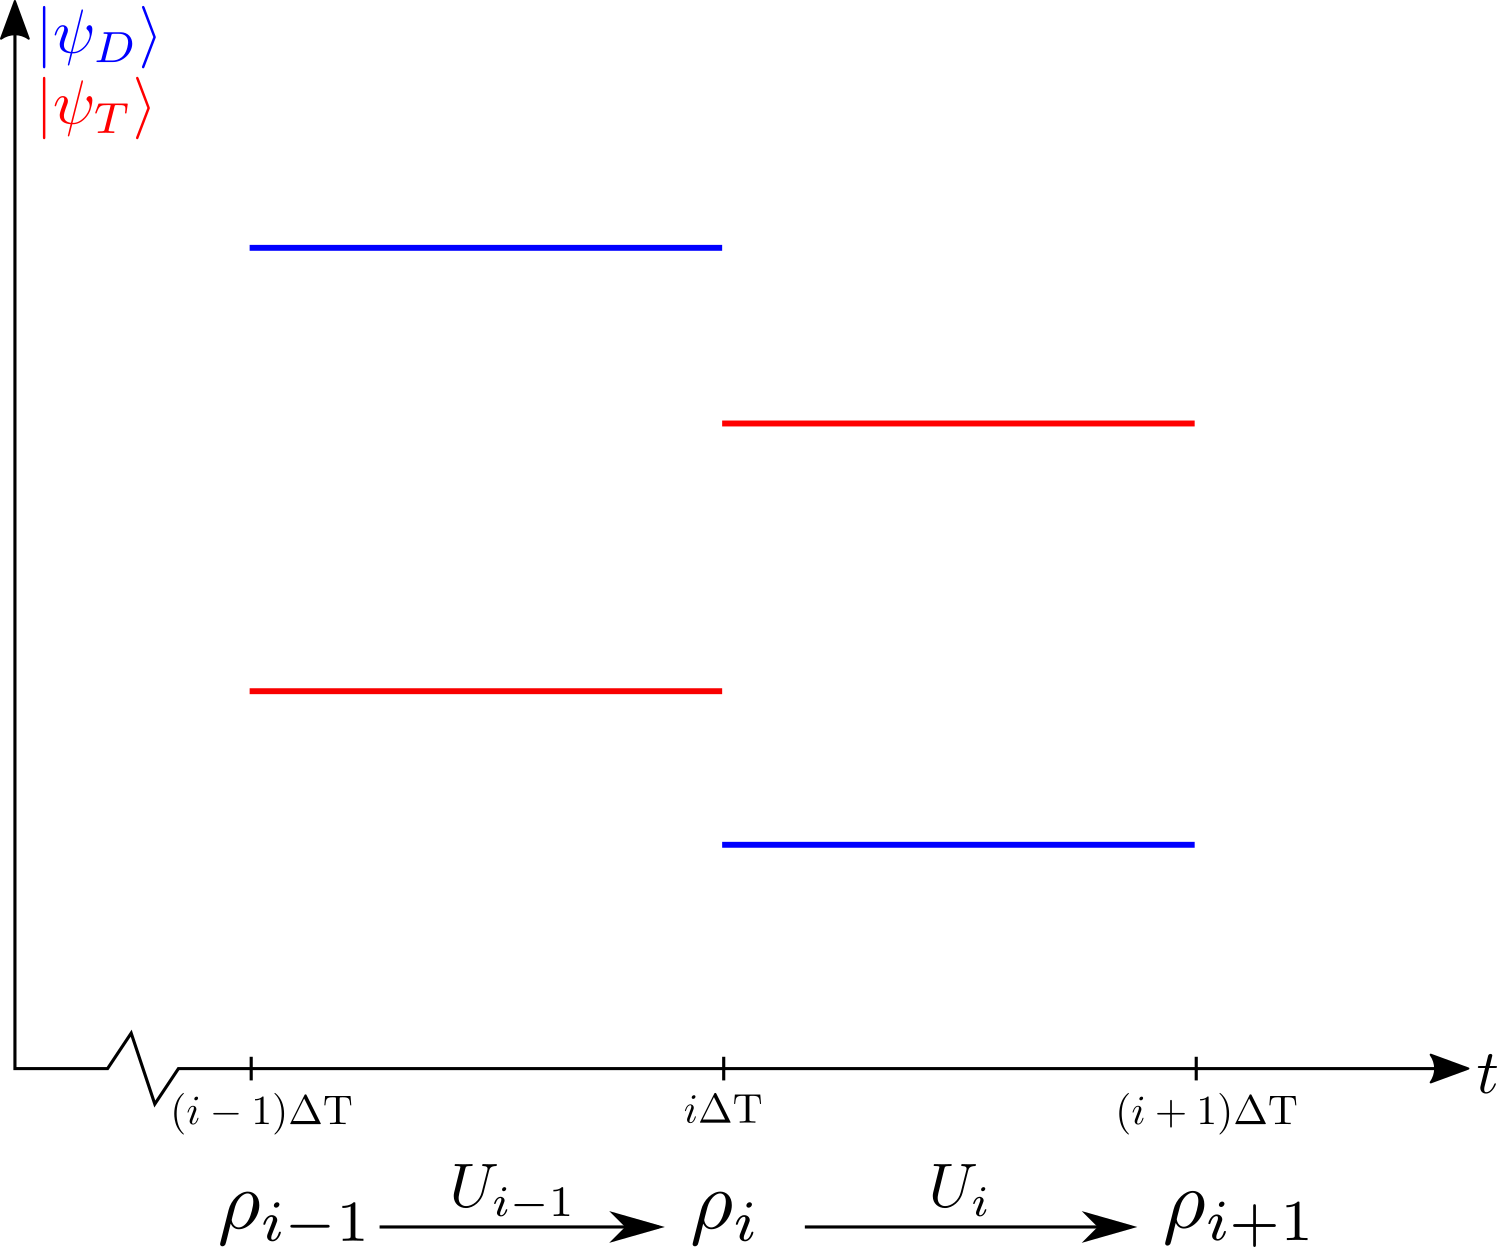
\includegraphics[width=0.6\textwidth]{img/pwc}
	\caption{Piecewise constant implementation of Drive and Transducer qubits: the vertical axis shows qubit state in arbitrary units. The qubit states are switched instantaneously and then kept constant for $\Delta \mathrm{T}$ while $\rho_S$ evolves unitarily.}
	\label{pwc}
\end{figure}

\begin{figure}
	\centering
	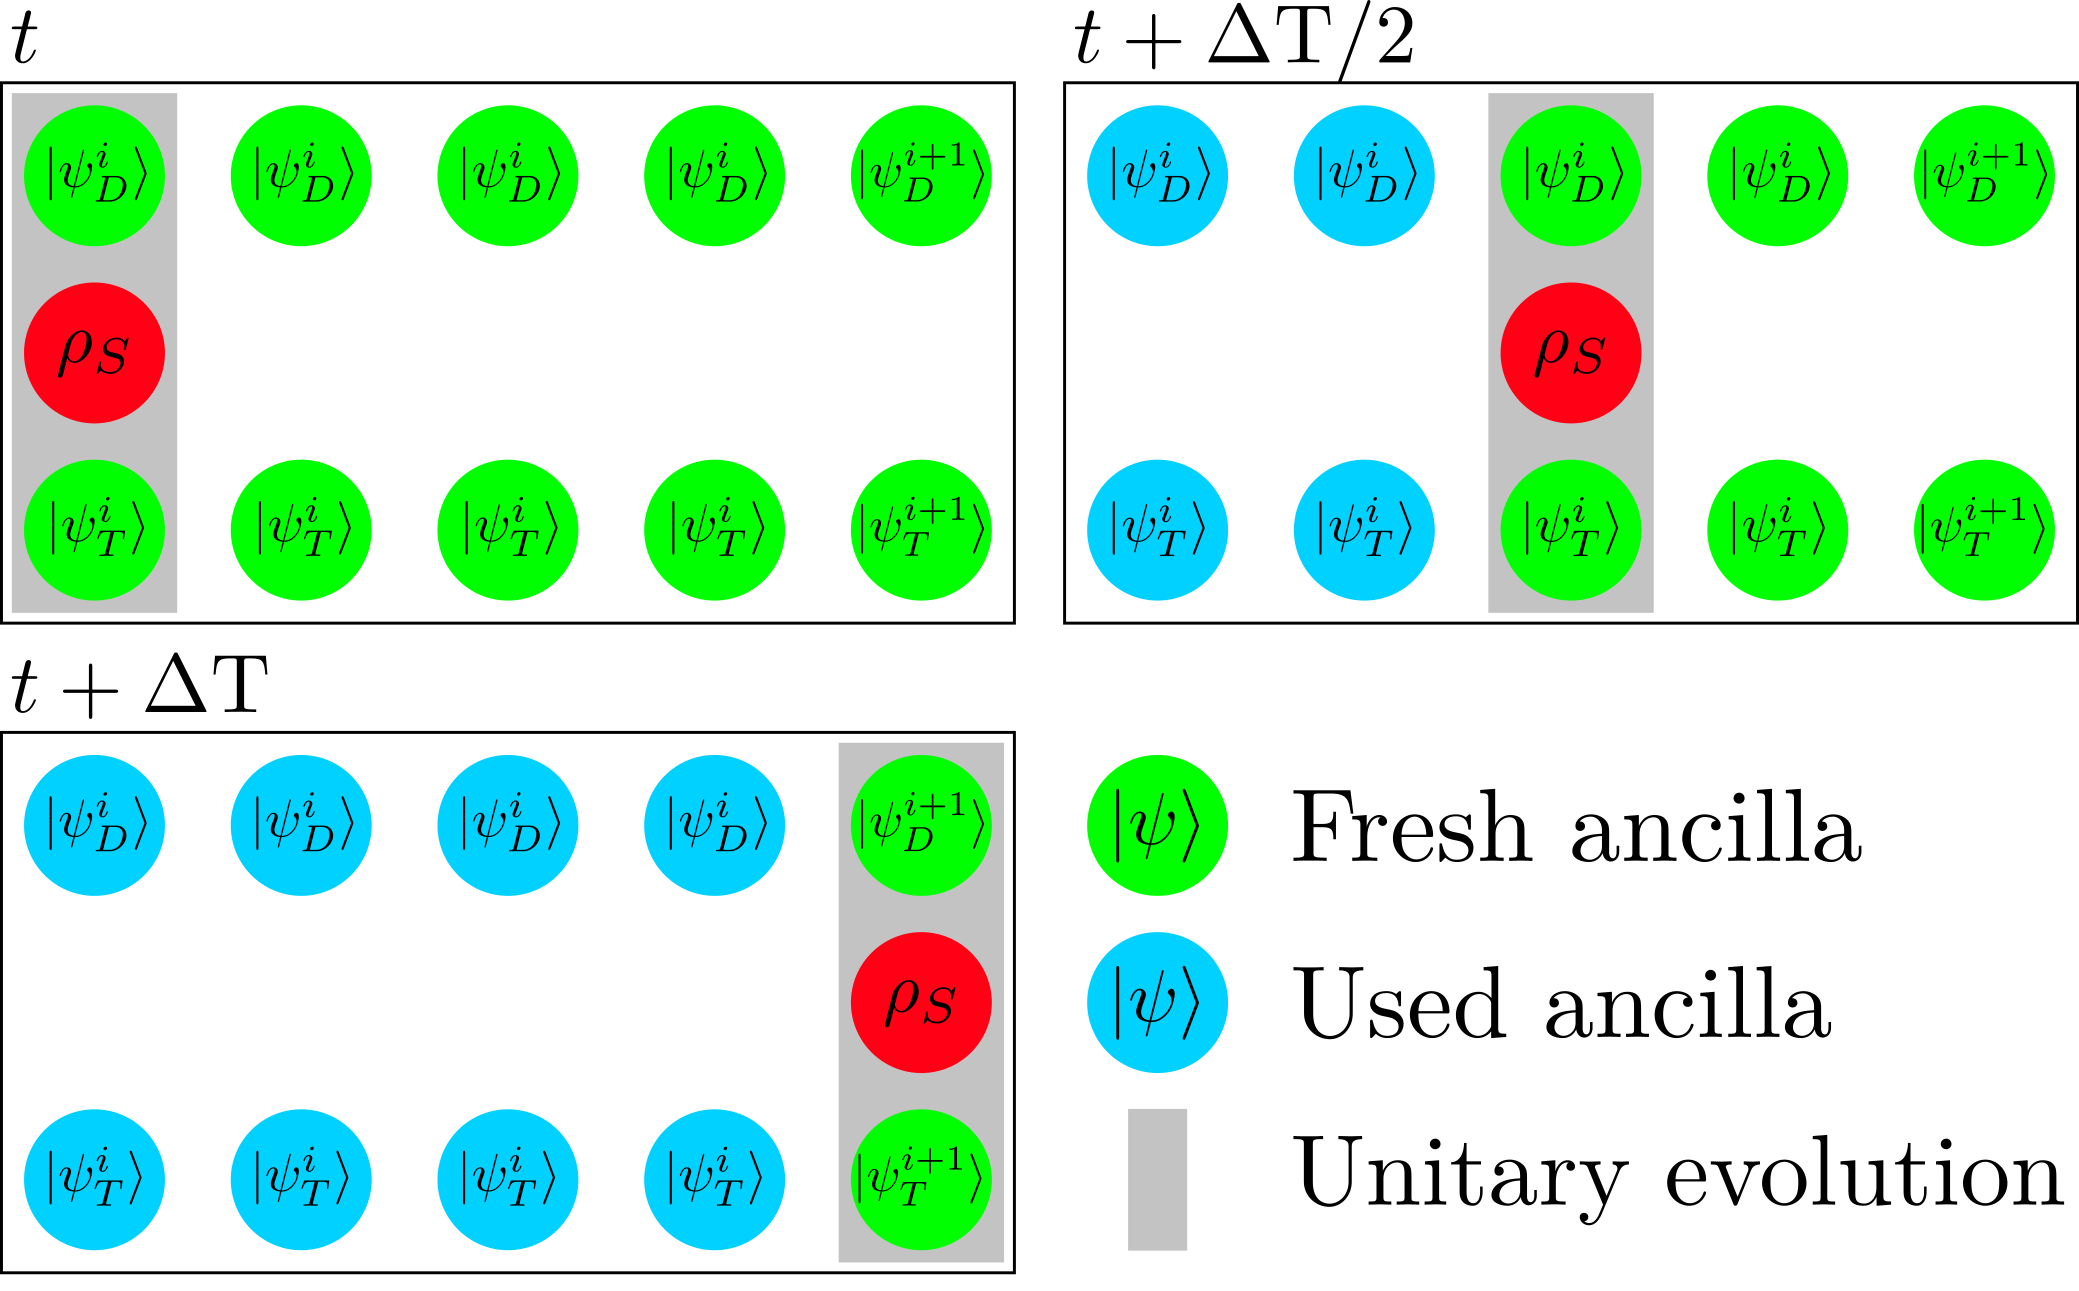
\includegraphics[width=0.7\textwidth]{img/collision_model}
	\caption{Collision model used in this work: Drive and Transducer are series of qubits interact once with the system and evolve the reduced density operator $\rho_S$. The qubit configuration can be changed in intervals of $\Delta \mathrm{T}$.}
	\label{collmodel}
\end{figure}
\section{Supervised machine learning} \label{sml}
Machine learning is a subfield of artificial intelligence, `concerned with the question of how to construct computer programs that automatically improve with experience.' \cite{Mitchell97}
Supervised machine learning is one of the three machine learning disciplines, besides unsupervised and reinforcement learning.
The goal is to find a mapping between an input and an output, in our case an excitation and its respective optimal harvesting policy.
Multiple algorithms to find such a mapping exist, however for high dimensional problems artificial neural networks (ANNs) are usually used.
In the following sections we review two ANN architectures, the fully-connected feedforward ANN and the Long Short-Term Memory (LSTM) network.

\subsection{Fully-connected feedforward ANNs}
In this section we review ANNs, following the exposition given in \cite{lu2020dying}.
Let $\textfrak{N}$ be a fully-connected feedforward ANN, meaning there are no loops in the neuron connections and all neurons in a layer are connected to every neuron of the next layer, $\textfrak{N}: \mathbb{R}^{n_1} \to \mathbb{R}^{n_L}$. $n_1$ and $n_L$ denote the dimensionality of the input and output respectively. 
$\textfrak{N}$ has $L$ layers, or columns of neurons.
The network architecture is given by the amount of neurons $n_l$ in each hidden layer $l \in [2, L - 1]$ (see figure \ref{nn}).
The neurons in layer $l$ are represented by their activations $\vec{a}_l \in \mathbb{R}^{n_l}$, which represent the matrix multiplication output. Additionally each layer includes trainable parameters $W_l \in \mathbb{R}^{n_{l+1} \times n_{l}}$ and $\vec{b}_l \in \mathbb{R}^{n_l}$ called weights and biases.
The activations can then be calculated using the following formulae \cite{TN_libero_mab2)53517}:
\begin{align*}
	\vec{a}_2 & = W_1 \vec{a}_1 + \vec{b}_1, \\
	\vec{a}_l & = W_{l-1} \xi(\vec{a}_{l-1}) + \vec{b}_{l-1}, \ l \in [3, L],
\end{align*}
where $\xi(x)$ is a function called the activation function applied elementwise. Historically, functions such as $\tanh$ and sigmoid have been used. However, it has been shown \cite{Maas2013RectifierNI, krizhevsky} that the rectified linear unit $\mathrm{ReLU}(x) = \mathrm{max}(0, x)$ often provides better results and is used here.


\subsection{Long Short-Term Memory}
While the network architecture introduced in the previous section performs reasonably well on many problems, it destroys spatial and temporal correlations present in the data. 
Instead convolutional and recurrent networks are often used for these purposes, e.g. in image recognition and time series forecasting \cite{rumelhart1986learning, 10.1007/978-3-642-46466-9_18}.

Here we use the LSTM architecture, a type of recurrent neural network (RNN) introduced in \cite{doi:10.1162/neco.1997.9.8.1735}. 
The core idea of RNNs is the usage of loops to store and propagate information through time.

The network is made up of a row of LSTM cells which share parameters.
The cell uses the current input $x_t$ as well as the previous cell state $c_{t-1}$ and output $h_{t-1}$ to compute the output $h_t$.
Internally, the cell is comprised of multiple gates which control the storage of information, $i_t, f_t, g_t, o_t$, which are the input, forget, cell and output gates respectively.
The output and gates of each cell are computed using the following equations:
\begin{align*}
i_t & = \sigma (W_{ii} x_t + b_{ii} + W_{hi} h_{t-1} + b_{hi}), \\
f_t & = \sigma (W_{if} x_t + b_{if} + W_{hf} h_{t-1} + b_{hf}), \\
g_t & = \tanh (W_{ig} x_t + b_{ig} + W_{hg} h_{t-1} + b_{hg}), \\ 
o_t & = \sigma (W_{if} x_t + b_{if} + W_{hf} h_{t-1} + b_{hf}), \\
c_t & = f_t \odot c_{t-1} + i_t \odot g_t, \\
h_t & = o_t \odot \tanh (c_t).
\end{align*}

\subsection{Training \& Backpropagation}
To train an ANN a cost function is defined, often the mean squared error 
\begin{align*}
	\mathrm{MSE} = \frac{1}{N} \sum_{i=1}^N (\vec{a}_{L, i} - \vec{y}_i)^2,
\end{align*}
where the summation is performed over the training data $\{(\vec{x}_i, \vec{y}_i)\}$ with $N$ samples, where $\{\vec{x_i}\}$ is the input and $\{\vec{y_i}\}$ the output data, and $\vec{a}_{L, i} = \textfrak{N}(\vec{x}_i)$ is the output of the neural network.
The so-called backpropagation algorithm is used to calculate the gradient of the cost function with respect to the trainable parameters and improve the performance of the ANN \cite{rumelhart1986learning, nielsenneural}.

\begin{figure}
	\centering
	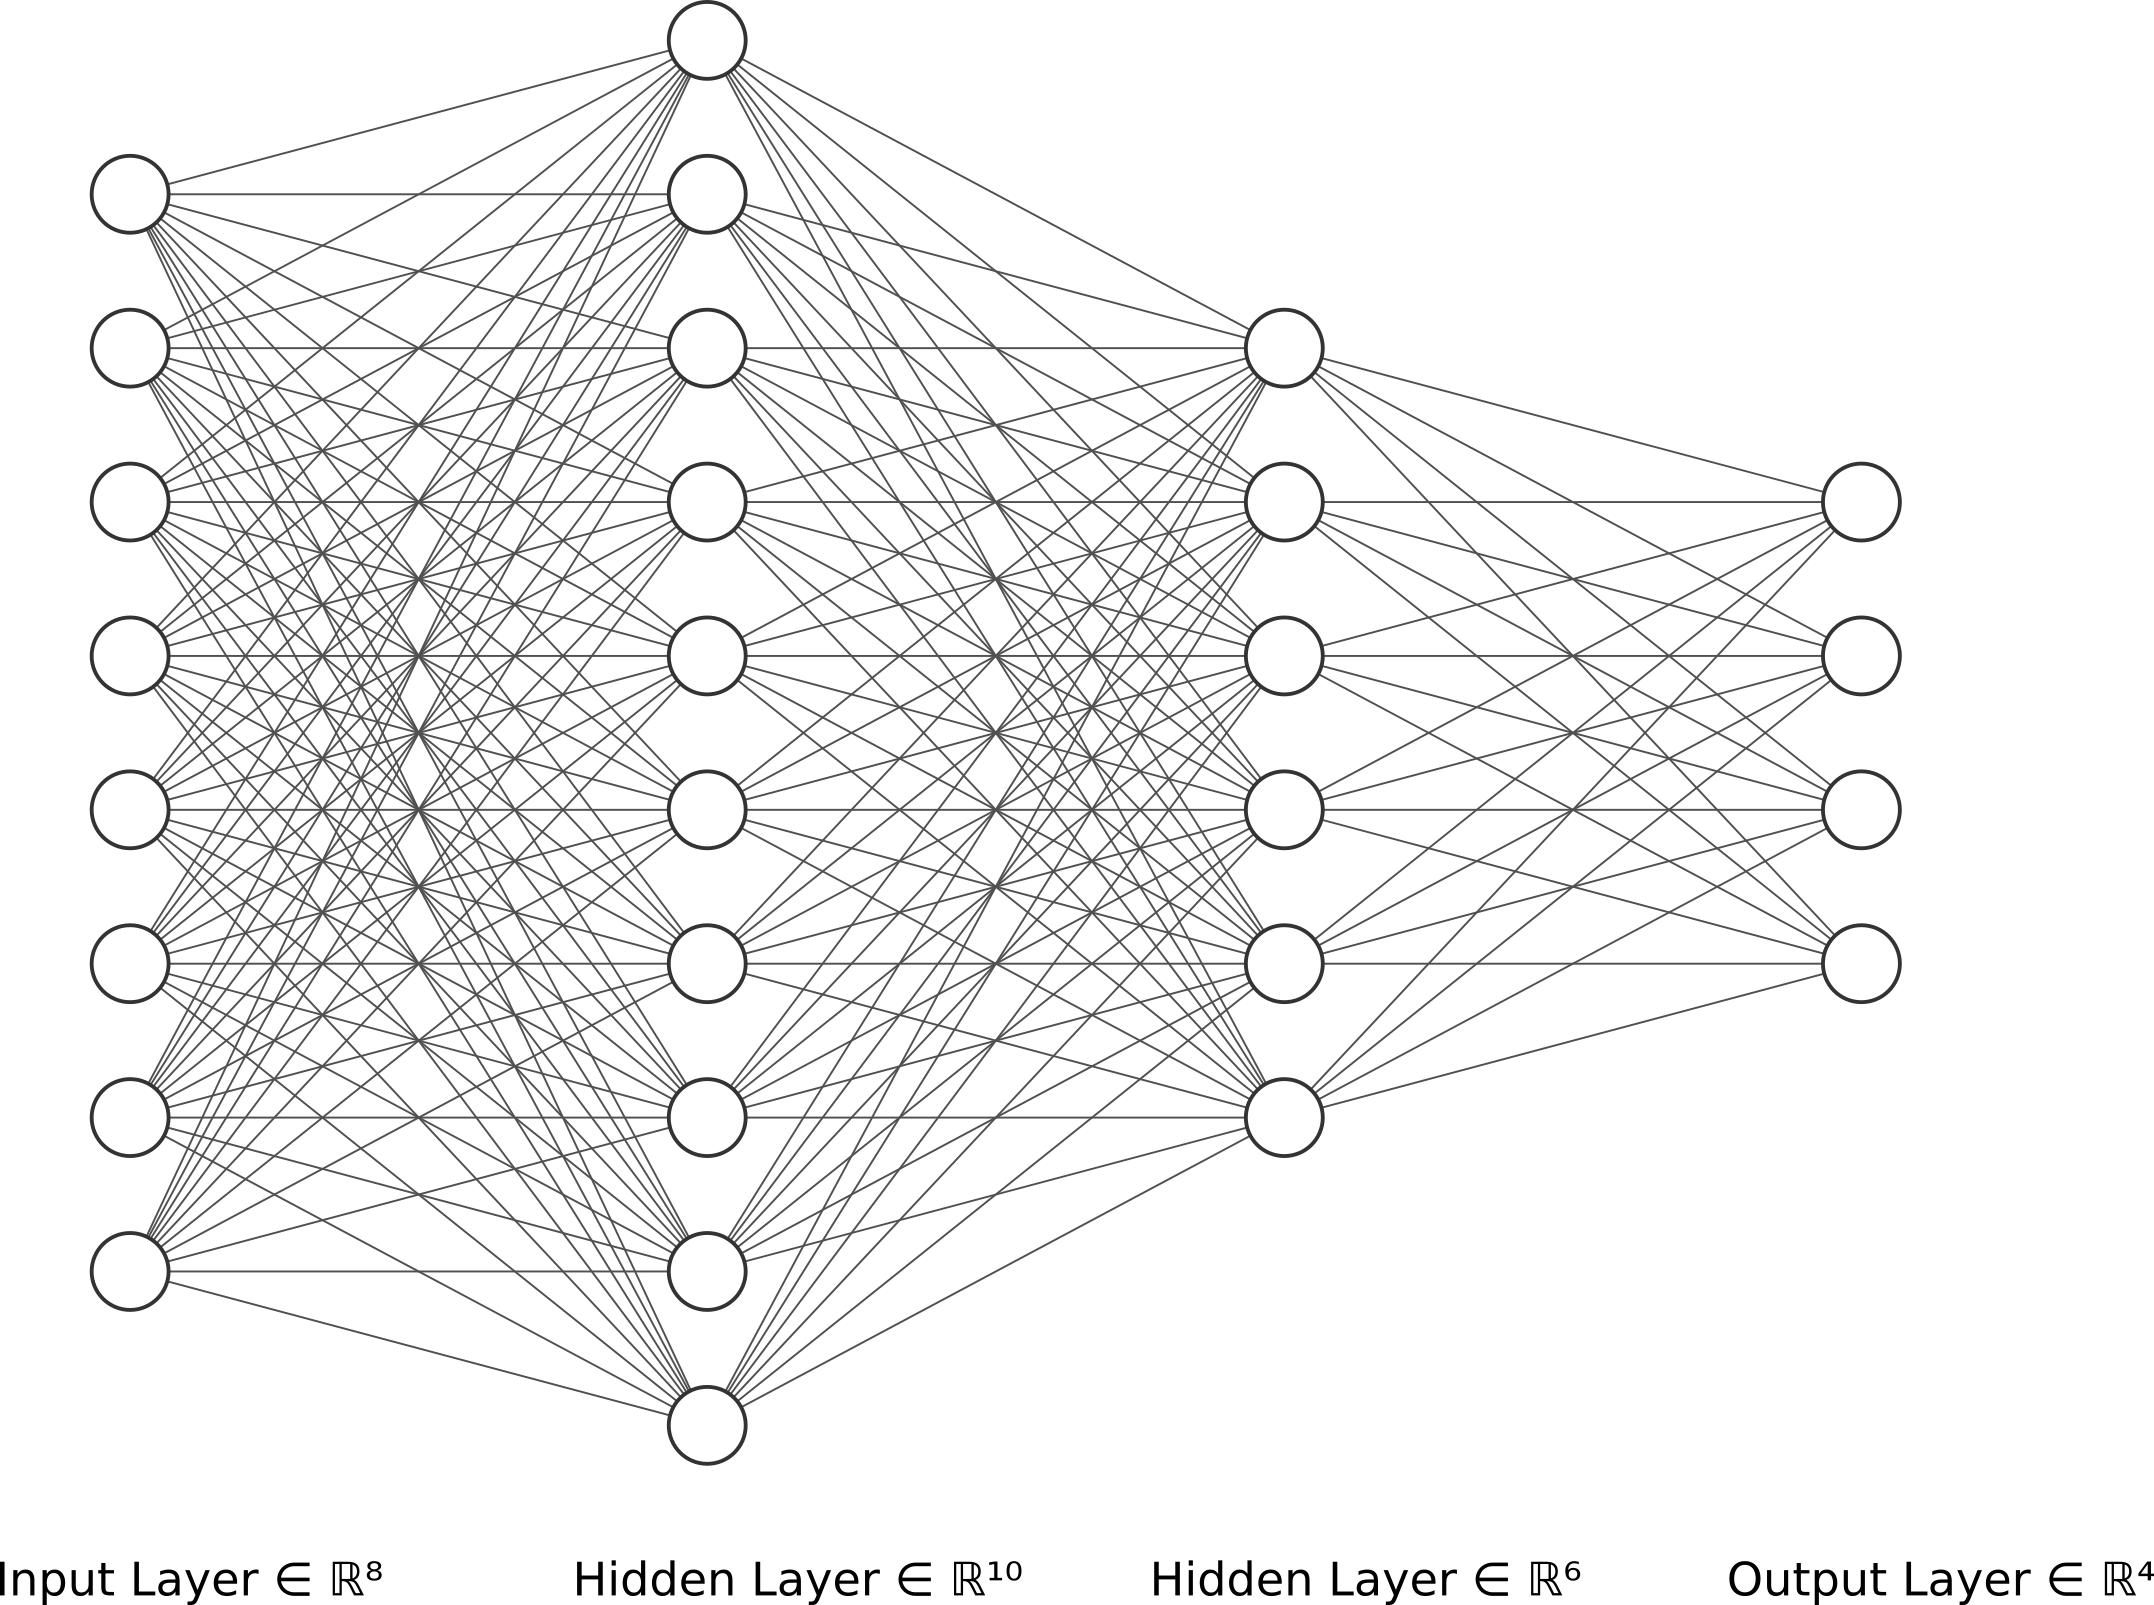
\includegraphics[width=0.6\textwidth]{img/nn}
	\caption{Example fully-connected feedforward ANN with four layers, including input, output and two hidden layers \cite{LeNail2019}}.
	\label{nn}
\end{figure}



\chapter{Work lower bound} \label{lower_bound}
% !TeX root = ../BA_main_englisch.tex
% !TeX spellcheck = en_GB
Before we apply neural networks, we derive a lower bound on the extractable work given a drive sequence $\{\ket{\psi_D^i}\}$.
By following a policy where the work output of each step $dW$ is optimised locally, we find that the transducer can be chosen such that $dW \geq 0$ for all drives.

We start in an arbitrary system state $\rho_S(n \Delta \mathrm{T})$.
Consider the evolved state $\rho_S((n+1) \Delta \mathrm{T}) =\frac{1}{2} (\mathds{1} + \vec{r} \cdot \vec{\sigma})$ after time $\Delta \mathrm{T}$, with $\vec{r} = ( x, y, z )$, where $\vec{r}$ would be determined by a unitary transformation in our case (note that the following is valid for any completely positive trace preserving (CPT) operation). According to Eqs. (\ref{dw}) and (\ref{simpledeltaham}), the step work output $dW_n$ is then given by
\begin{align*}
dW_n &= \Tr{\rho_S((n+1) \Delta \mathrm{T}) (H_{ST}^{n} - H_{ST}^{n+1})} \\
&= \Tr{\rho_S((n+1) \Delta \mathrm{T}) \left((\Re{\tau^n} - \Re{\tau^{n+1}}) \sigma_x + (\Im{\tau^n} - \Im{\tau^{n+1}} ) \sigma_y \right)} \\
&= x (\Re{\tau^n} - \Re{\tau^{n+1}}) + y (\Im{\tau^n} - \Im{\tau^{n+1}}), \\
\tau^n &= \frac{1}{2} \sin{\theta_T^n} e^{i\phi_T^n}. 
\end{align*}
$\tau^n$ is determined by the previous step and thus we can only vary $\tau^{n+1}$.
$dW_n$ has a maximum for $\theta_T^{n+1} = \frac{\pi}{2}, \ \phi_T^{n+1} = \arctan{\frac{y}{x}} + \pi$, giving
\begin{align*}
dW_{n, lo} &= \frac{1}{2}\left(\sqrt{x^2 + y^2} + \sin(\theta^n_T) \begin{pmatrix} \cos(\phi^n_T) \\ \sin(\phi^n_T) \end{pmatrix} \cdot \begin{pmatrix} x \\ y \end{pmatrix} \right) \\
 &\geq \frac{1}{2}\left(\sqrt{x^2 + y^2} - \abs{ \begin{pmatrix} \cos(\phi^n_T) \\ \sin(\phi^n_T) \end{pmatrix} \cdot \begin{pmatrix} x \\ y \end{pmatrix}} \right) \\
 &\geq \frac{1}{2}\left(\sqrt{x^2 + y^2} - \sqrt{x^2 + y^2} \right) = 0,
\end{align*}
where we used the Cauchy-Schwarz inequality going from the second to the third line.

In our setting, $\vec{r}$ only depends on the current $\ket{\psi_D}$ and $\rho_S$.
For a given drive sequence the sum of the locally optimised work outputs $dW_{n, lo}$ provides a lower bound on the total extractable work as each contribution is non-negative. In the following chapter we will show that protocols with higher outputs exist by optimising globally over all time steps.

\chapter{Simulation results}
\section{Influence of $\Delta \mathrm{T}$ on Work Output} \label{dep_dt}
% !TeX spellcheck = en_GB
We start our investigation by determining the work output $W$ when varying the time between qubit switching $\Delta \mathrm{T}$.
If the system qubit is initialised in the pure state $\rho_S = \ket{0} \bra{0}$, the work output for a single jump is given by (see appendix \ref{deriv_jump} for a derivation)
\begin{equation} \label{single_work}
	W = \frac{1}{\abs{\alpha}} \sin(2\abs{\alpha}\Delta \mathrm{T}) \Im{(\tau' - \tau) \alpha^*}
\end{equation}
\begin{equation*}
	\alpha = \frac{1}{2} \left[\sin(\theta_D^1) e^{i\phi_D^1} + \sin(\theta_T^1) e^{i\phi_T^1}\right], \\
	\tau' - \tau = \frac{1}{2} \left[ \sin(\theta_T^2)e^{i\phi_T^2} - \sin(\theta_T^1)e^{i\phi_T^1} \right].
\end{equation*}

We note that for $\Delta \mathrm{T} \to 0, \ W \to 0$ as $\Tr{\rho_S H_S} = 0$ for all configurations of $\ket{\psi_D}$ and $ \ket{\psi_T}$.
We simulate 500 random drive functions for multiple values of $N$ and each $\Delta \mathrm{T}$, finding their optimal transducer policy. The average work output over the 500 runs scaled by the number of work extractions $\overline{W}/(N-1)$ for 20 values of $\Delta \mathrm{T}$ is shown in Figure \ref{dt_0}.

In Figure \ref{dt_eigen}, we plot the average work when the system qubit is initialised in an eigenstate $\rho_0 = \ket{+}\bra{+}$ of the partial system Hamiltonian $H_{DS}$.
For $\Delta \mathrm{T} = 0$, the work output is $W = 1$ for all $N$. This is the amount of work that can be extracted by switching the Hamiltonian in such a way that the eigenvalues change signs.
A special case occurs for $N = 2$: the optimal case is independent of $\Delta \mathrm{T}$.
Here, the maximum work output per step of $W = 1$ can be achieved by setting the transducer such that the total system Hamiltonian commutes with $H_{DS}$. $\rho_S$ remains in the eigenstate and after time $\Delta \mathrm{T}$, \ $W = 1$ can be extracted from the system as with $\Delta \mathrm{T} = 0$.

For both initial system states and large $N$ and $\Delta \mathrm{T}$, the maximum work per extraction step $\frac{\overline{W}}{N-1} = 0.5$.
For smaller $\Delta \mathrm{T}$, the work per extraction step is lower, as the optimal system state cannot be reached due to the speed limit in unitary dynamics \cite{Deffner_2017, PhysRevA.67.052109}.

\begin{figure}[h]
	\centering
	\begin{subfigure}{0.4\textwidth}
		\centering
		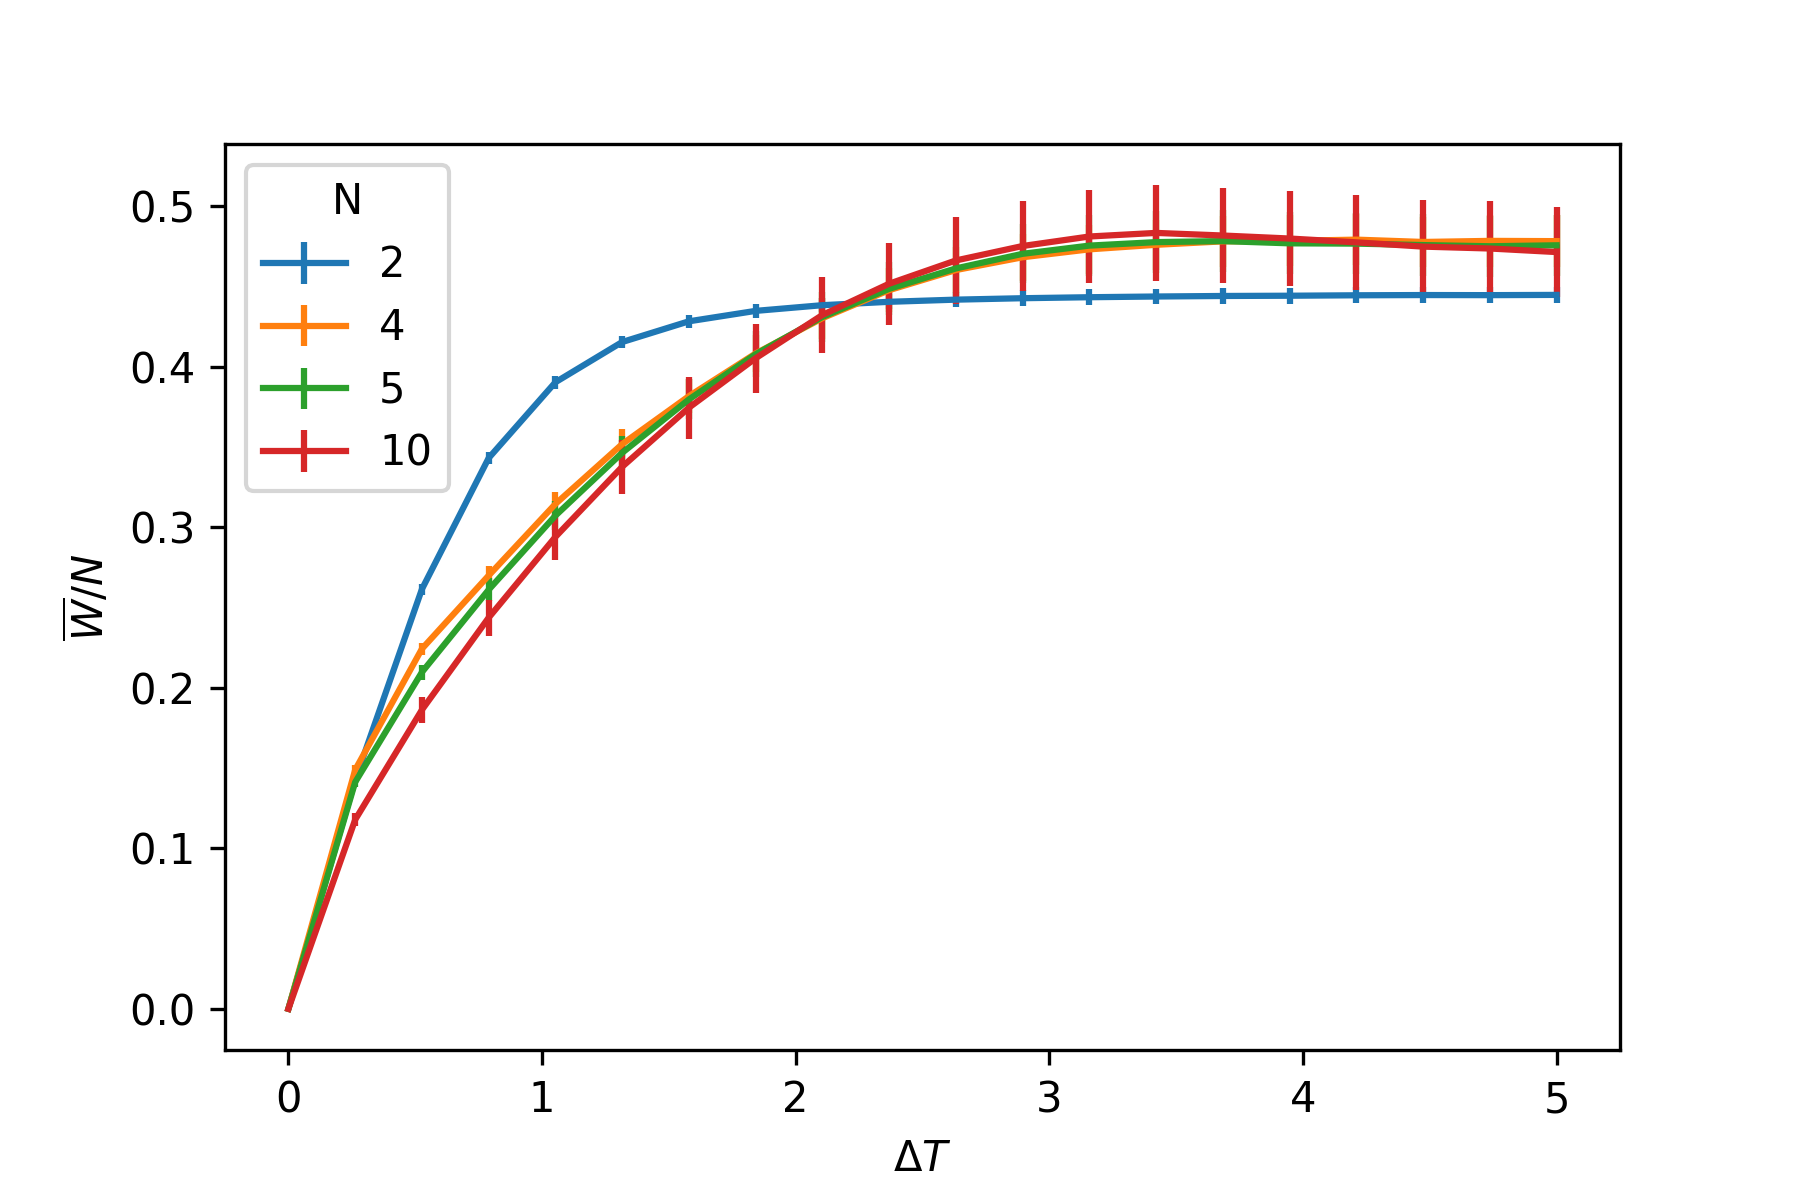
\includegraphics[width=\textwidth]{img/dt_0}
		\caption{$\rho_0 = \ket{0}\bra{0}$}
		\label{dt_0}
	\end{subfigure}
	\begin{subfigure}{0.4\textwidth}
	\centering
	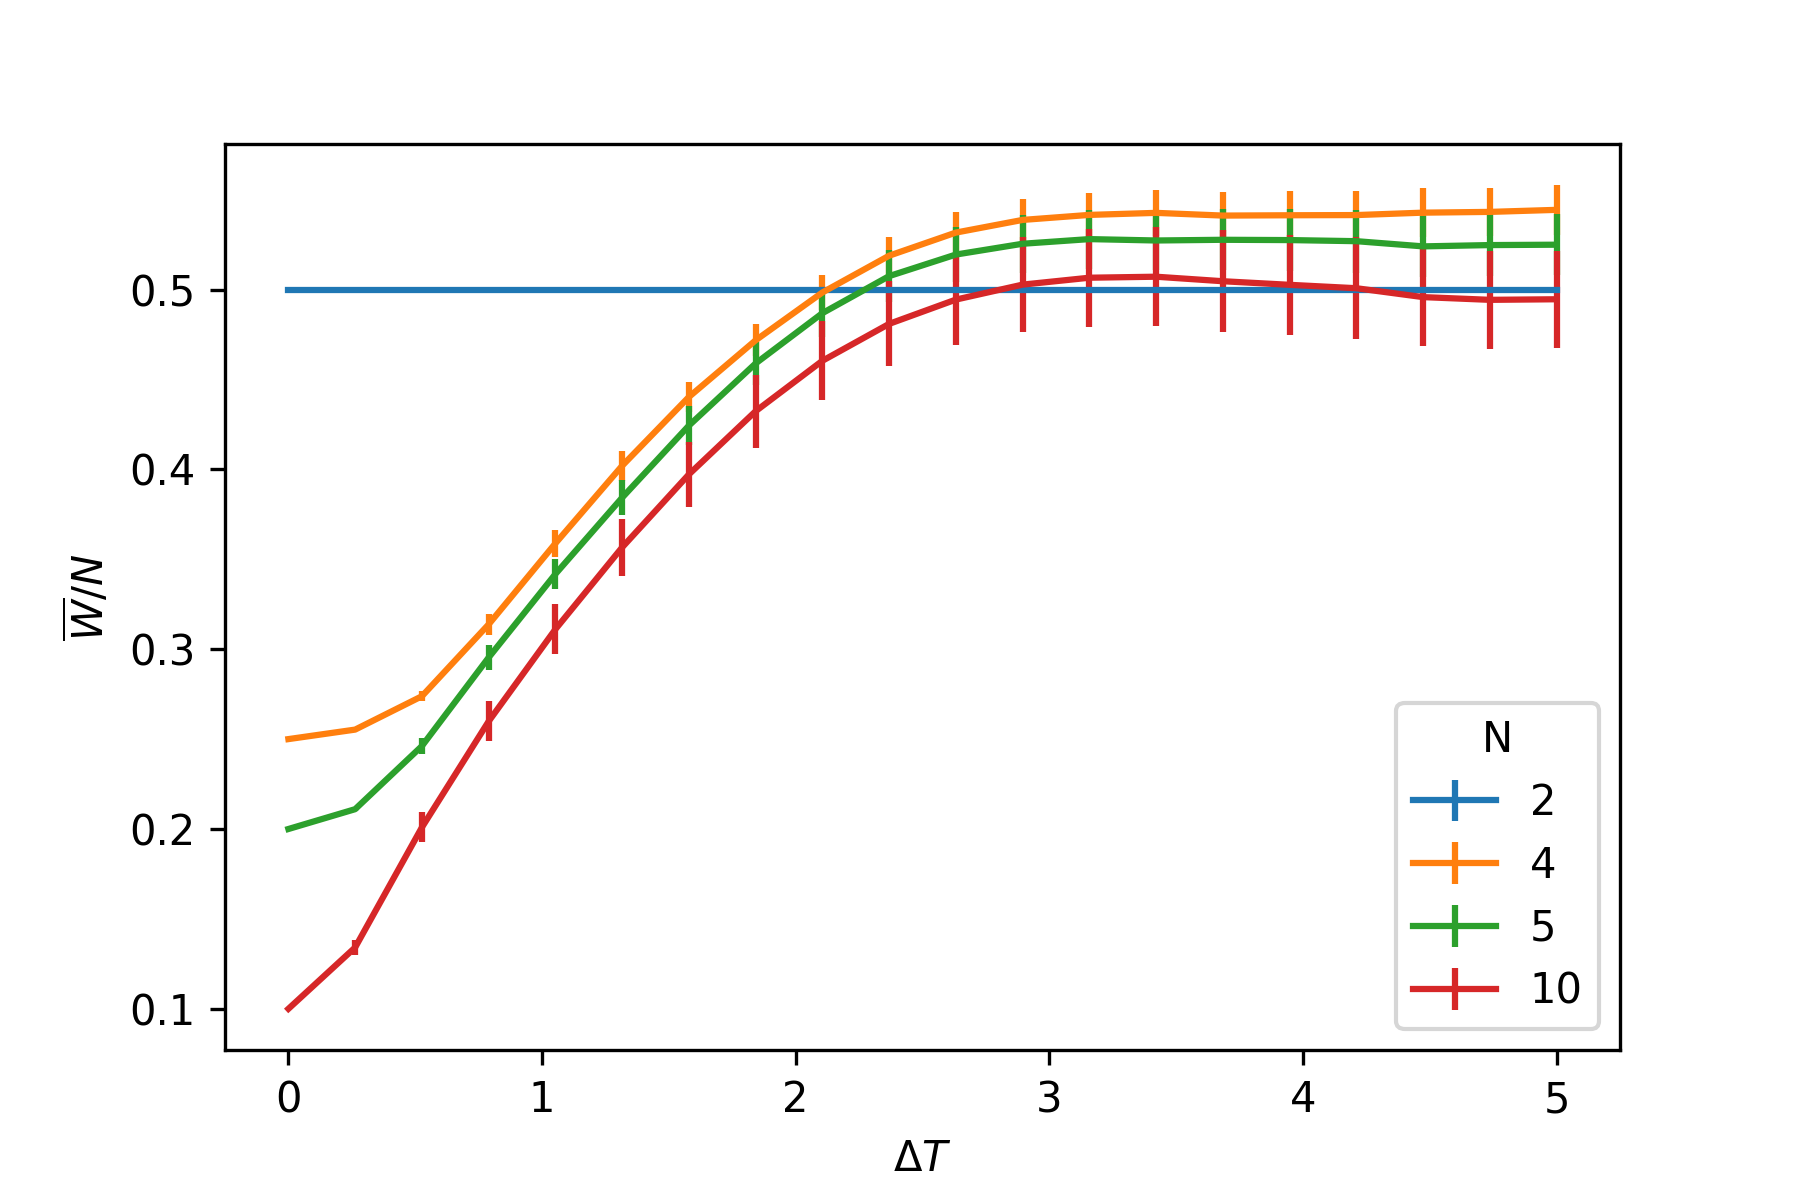
\includegraphics[width=\textwidth]{img/dt_eigen}
	\caption{$\rho_0 = \ket{+}\bra{+}$}
	\label{dt_eigen}
	\end{subfigure}
	\caption{(a) We plot the average work $\overline{W}$ over $n = 500$ runs of random excitations divided by amount of qubit changes $N - 1$, with $\rho_0 = \ket{0}\bra{0}$, for multiple $N$. The error bars correspond to the standard deviation $\sigma_{W} = \sqrt{\frac{1}{n-1} \Sigma_i^n (\overline{W} - W_i)^2}$.
	(b) We plot $\overline{W}/(N-1)$ for multiple $N$ where the system state is initialised in an eigenstate of the drive Hamiltonian $H_{DS}$.}
	\label{dt_dep}
\end{figure}
\section{Data creation, training and evaluation} \label{data_create}
The training data is created using a minimisation algorithm \cite{2020SciPy-NMeth}, which finds the optimal transducer protocol $\{|\psi_T^i \rangle\}$ given a drive sequence $\{|\psi_D^i \rangle\}$.
The networks are trained to learn the mapping $\{|\psi_D^i \rangle\} \to \{|\psi_T^i \rangle\}$.
Both the input (drive) and output (transducer) are transformed by the embedding
\begin{align*}
	\left\{
	\begin{pmatrix}
	\theta^n & \phi^n \\
	\end{pmatrix}
	\right\}
	\to
	\left\{
	\begin{pmatrix}
	\sin(\theta^n) & \sin(\phi^n) & \cos(\theta^n)  & \cos(\phi^n) \\
	\end{pmatrix}
	\right\}.
\end{align*}
The reasons for this operation are twofold: it normalises the data to the interval $[-1, 1]$, which is beneficial to learning \cite{LeCun2012}. Additionally it encodes information regarding the periodicity of the qubit angle representation.
We add either a zero or a one as an extra input parameter for LSTM training depending on whether or not the input is the last in a sequence.

To compare the accuracy of different models a performance indicator is required. 
Naturally one might use the MSE as introduced in section \ref{sml}.
Instead we define the \textit{efficiency} of a model $\textfrak{N}$ on a dataset $\{(\vec{x}_i, \vec{y}_i)\}$ as
\begin{align}
	\eta = \frac{1}{N} \sum_{i=1}^N \frac{W(\vec{x}_i,\textfrak{N}(\vec{x}_i))}{W(\vec{x}_i,\vec{y}_i)},
\end{align}
i.e. the arithmetic mean of the ratios of work output predicted by the model to optimal work output.
The function $W(\vec{x}_i, \vec{y}_i) = W(\{\ket{\psi_D^n}\}_i, \{\ket{\psi_T^n}\}_i)$ returns the work given a drive and transducer sequence.

It should be noted that using the MSE for training is not the only choice, and perhaps not the obvious one.
Directly using the work extracted is possibly a more intuitive choice, but we refrain from it in the first section for two main reasons.
Firstly, the interaction Hamiltonian must be known to the experimenter for use as a cost function.
Secondly, the computation of the extracted work becomes costly for larger $N$, as calculating the work is $O(N-1)$ while MSE $= O(1)$.
\section{Amount of qubit switches $N=2$: Learning single extraction step optimal control sequences} \label{n_2_ml}
% !TeX spellcheck = en_GB
For the simplest case of $N = 2$, we generate data sets of size $N_{\mathrm{data}} = 20000$ for $\rho_0 = \ket{0} \bra{0}, \ket{+} \bra{+}$ and random pure states.
The drive qubits are sampled randomly from the Haar measure \cite{Mezzadri}.
We train each data set on a fully-connected feedforward ANN with a single hidden layer with 10 neurons.
The efficiency of the models is presented in table \ref{n2efftable}.
For $N = 2$, starting in an eigenstate of the drive Hamiltonian $H_{DS}$ gives the highest model efficiency, as the optimal Transducer policy is trivial to learn and implement (see appendix \ref{n2_opt_pol}).

For random initial states the efficiency is close to zero.
This is to be expected, as without knowledge of the system state $\rho_0$ the optimal Transducer policy cannot be determined.\footnote{The deviation from zero is a relic of the way the test data is shuffled. For $N_{\mathrm{data}} \to \infty$ it would disappear.}
We therefore train the same network with the random initial state as additional inputs using the same embedding as the Drive sequence.
This increases the test data efficiency, but is still far below the efficiency for $\rho_0 = \ket{+} \bra{+}$.


\begin{table}[h]
	\centering
	\begin{tabular}{ c | c }
		$\rho_0$ & $\eta_{test} \ [\%]$ \\
		\hline
		$\ket{0} \bra{0}$ & 72.7 \\
		$\ket{+} \bra{+}$ & 100.0 \\
		Random & 0.5 \\
		Random, $\rho_0$ as input & 43.0 \\
	\end{tabular}
	\caption{Efficiencies $\eta$ on the test data for models with a single hidden layer with 10 neurons trained on drive protocols with $N = 2$ and differing initial states $\rho_0$.}
	\label{n2efftable}
\end{table}


%\begin{figure}
%	\centering
%	\begin{subfigure}{0.4\textwidth}
%		\centering
%		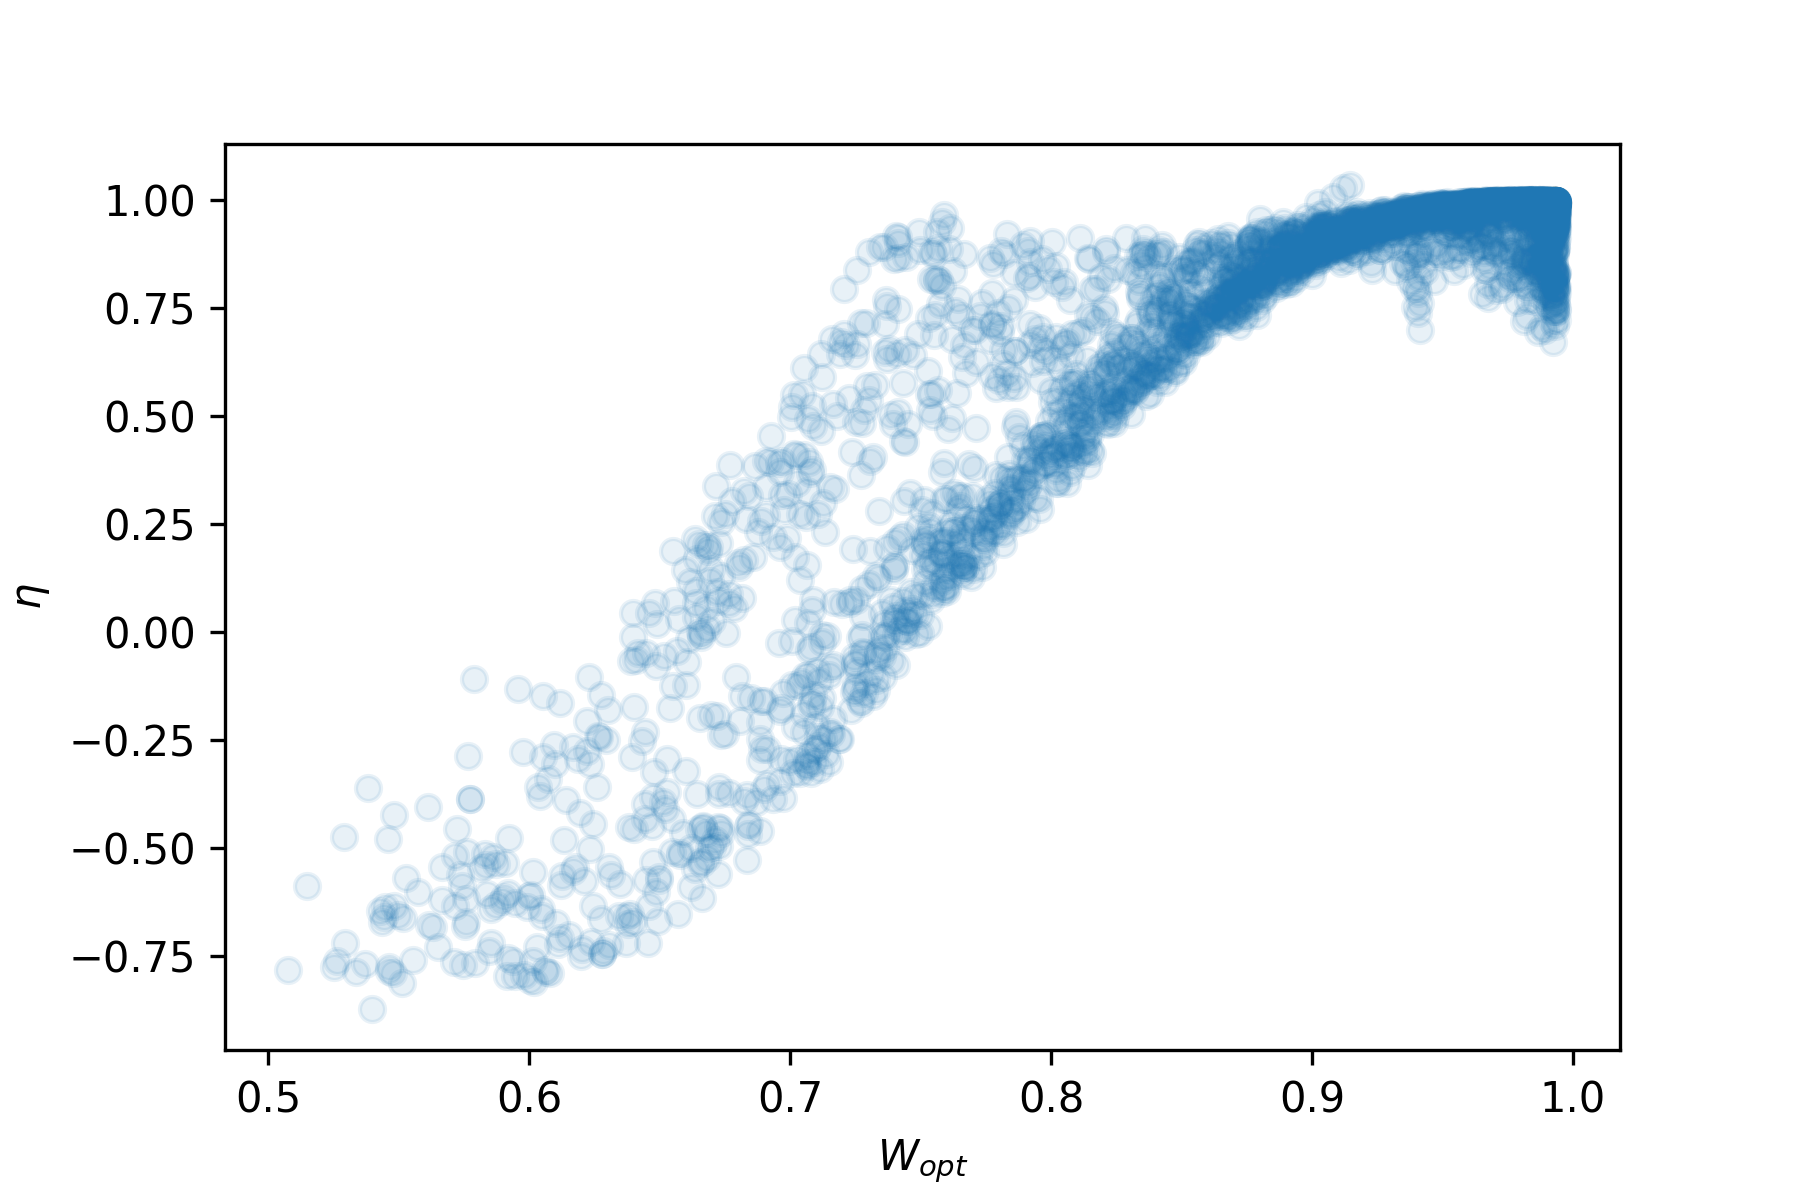
\includegraphics[width=\textwidth]{img/work_dist_n2_0}
%		\caption{$\rho_0 = \ket{0}\bra{0}$}
%		\label{}
%	\end{subfigure}
%	\begin{subfigure}{0.4\textwidth}
%		\centering
%		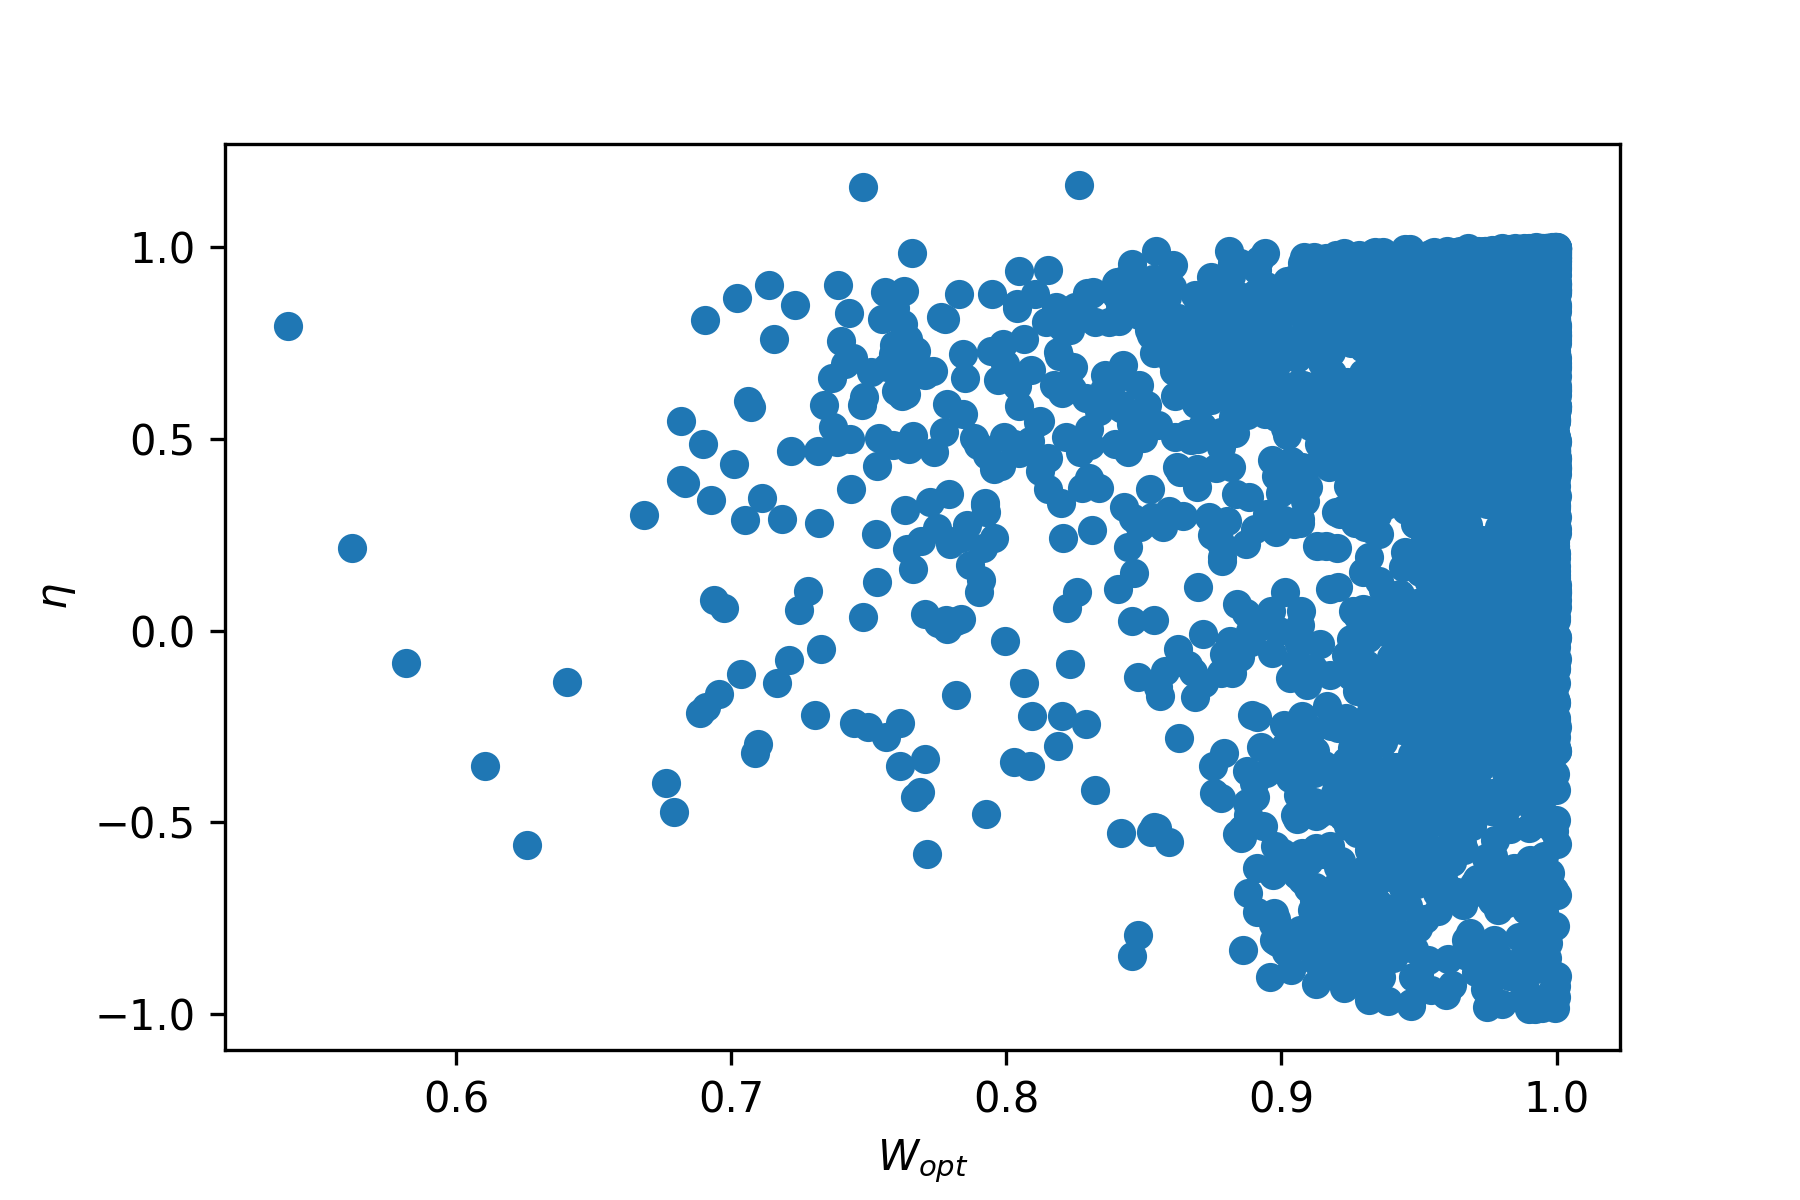
\includegraphics[width=\textwidth]{img/work_dist_n2_haar}
%		\caption{Random $\rho_0$}
%		\label{}
%	\end{subfigure}
%	\caption{}
%	\label{}
%\end{figure}
%
%
%\begin{figure}
%	\centering
%	\begin{subfigure}{0.4\textwidth}
%		\centering
%		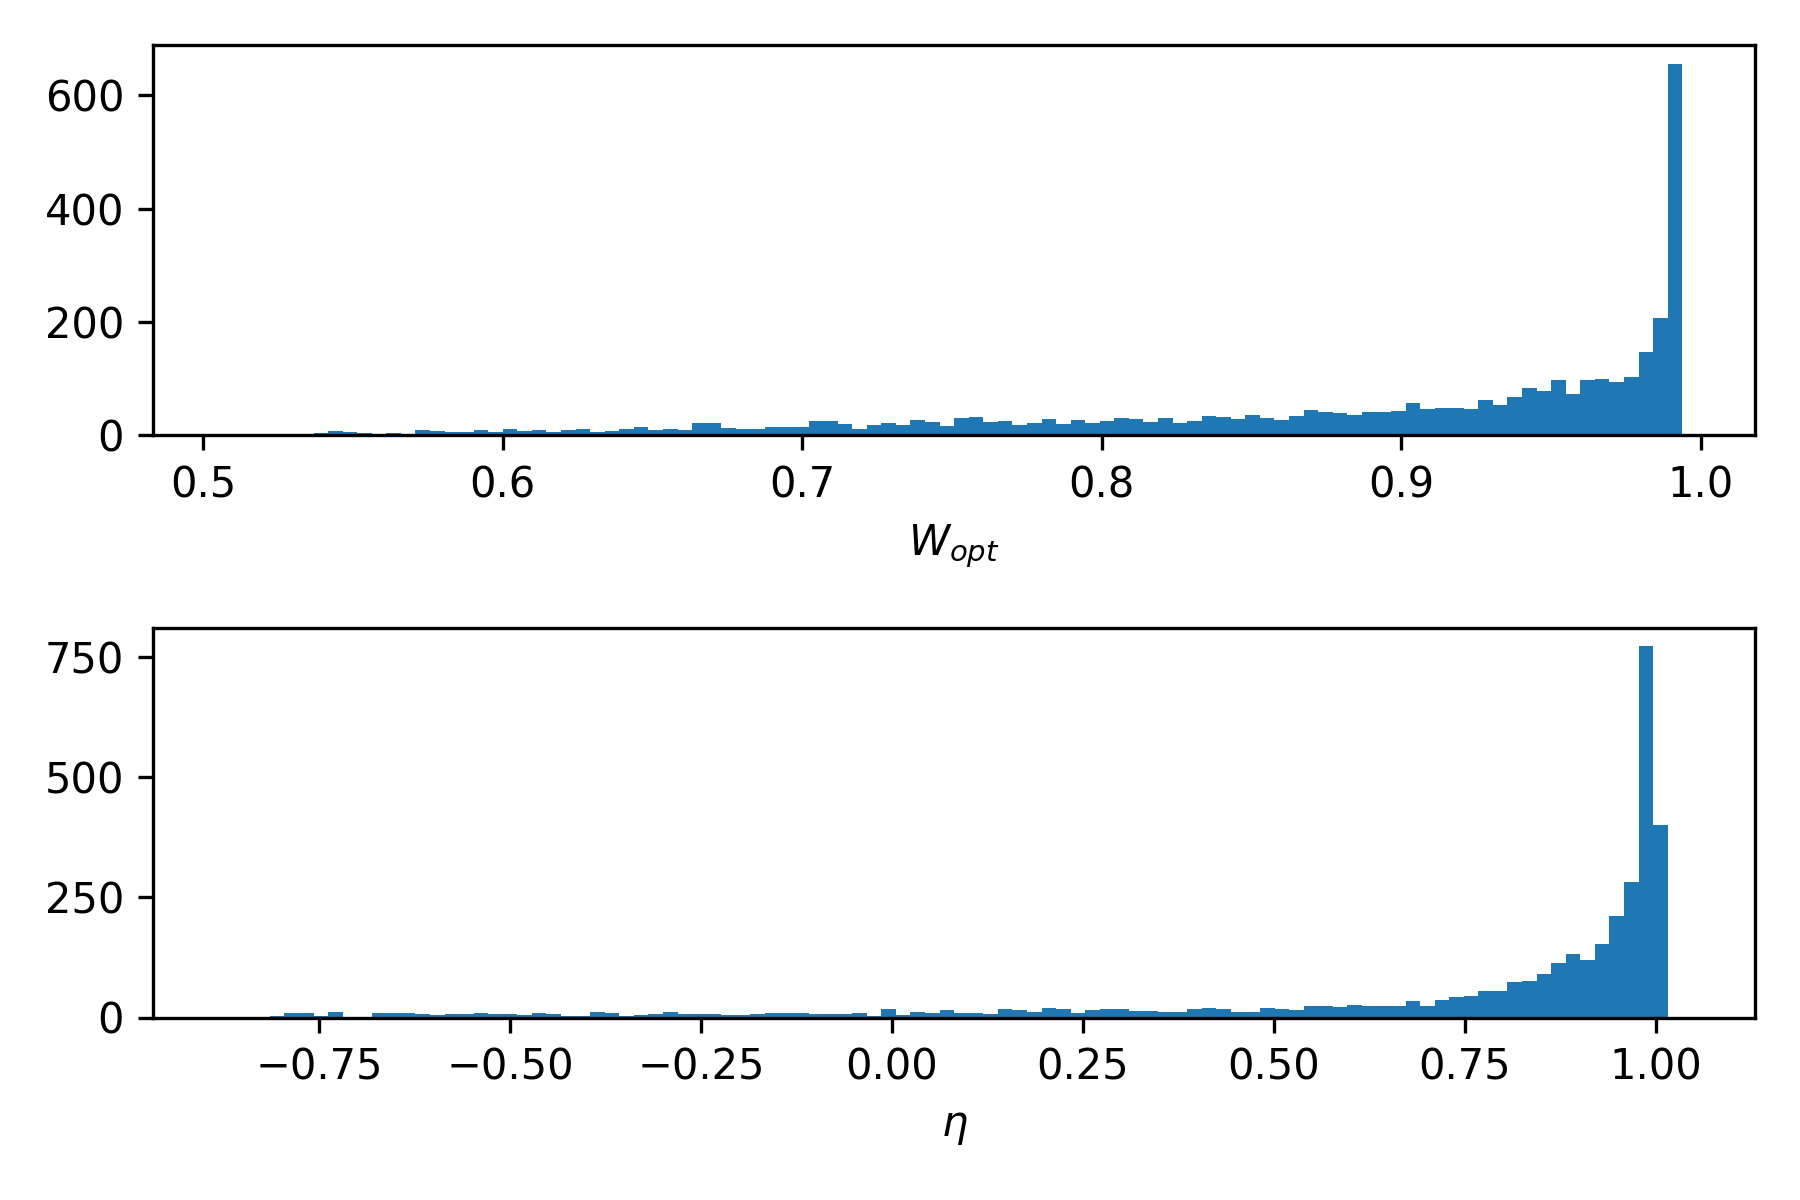
\includegraphics[width=\textwidth]{img/hist_n2_0}
%		\caption{$\rho_0 = \ket{0}\bra{0}$}
%		\label{}
%	\end{subfigure}
%	\begin{subfigure}{0.4\textwidth}
%		\centering
%		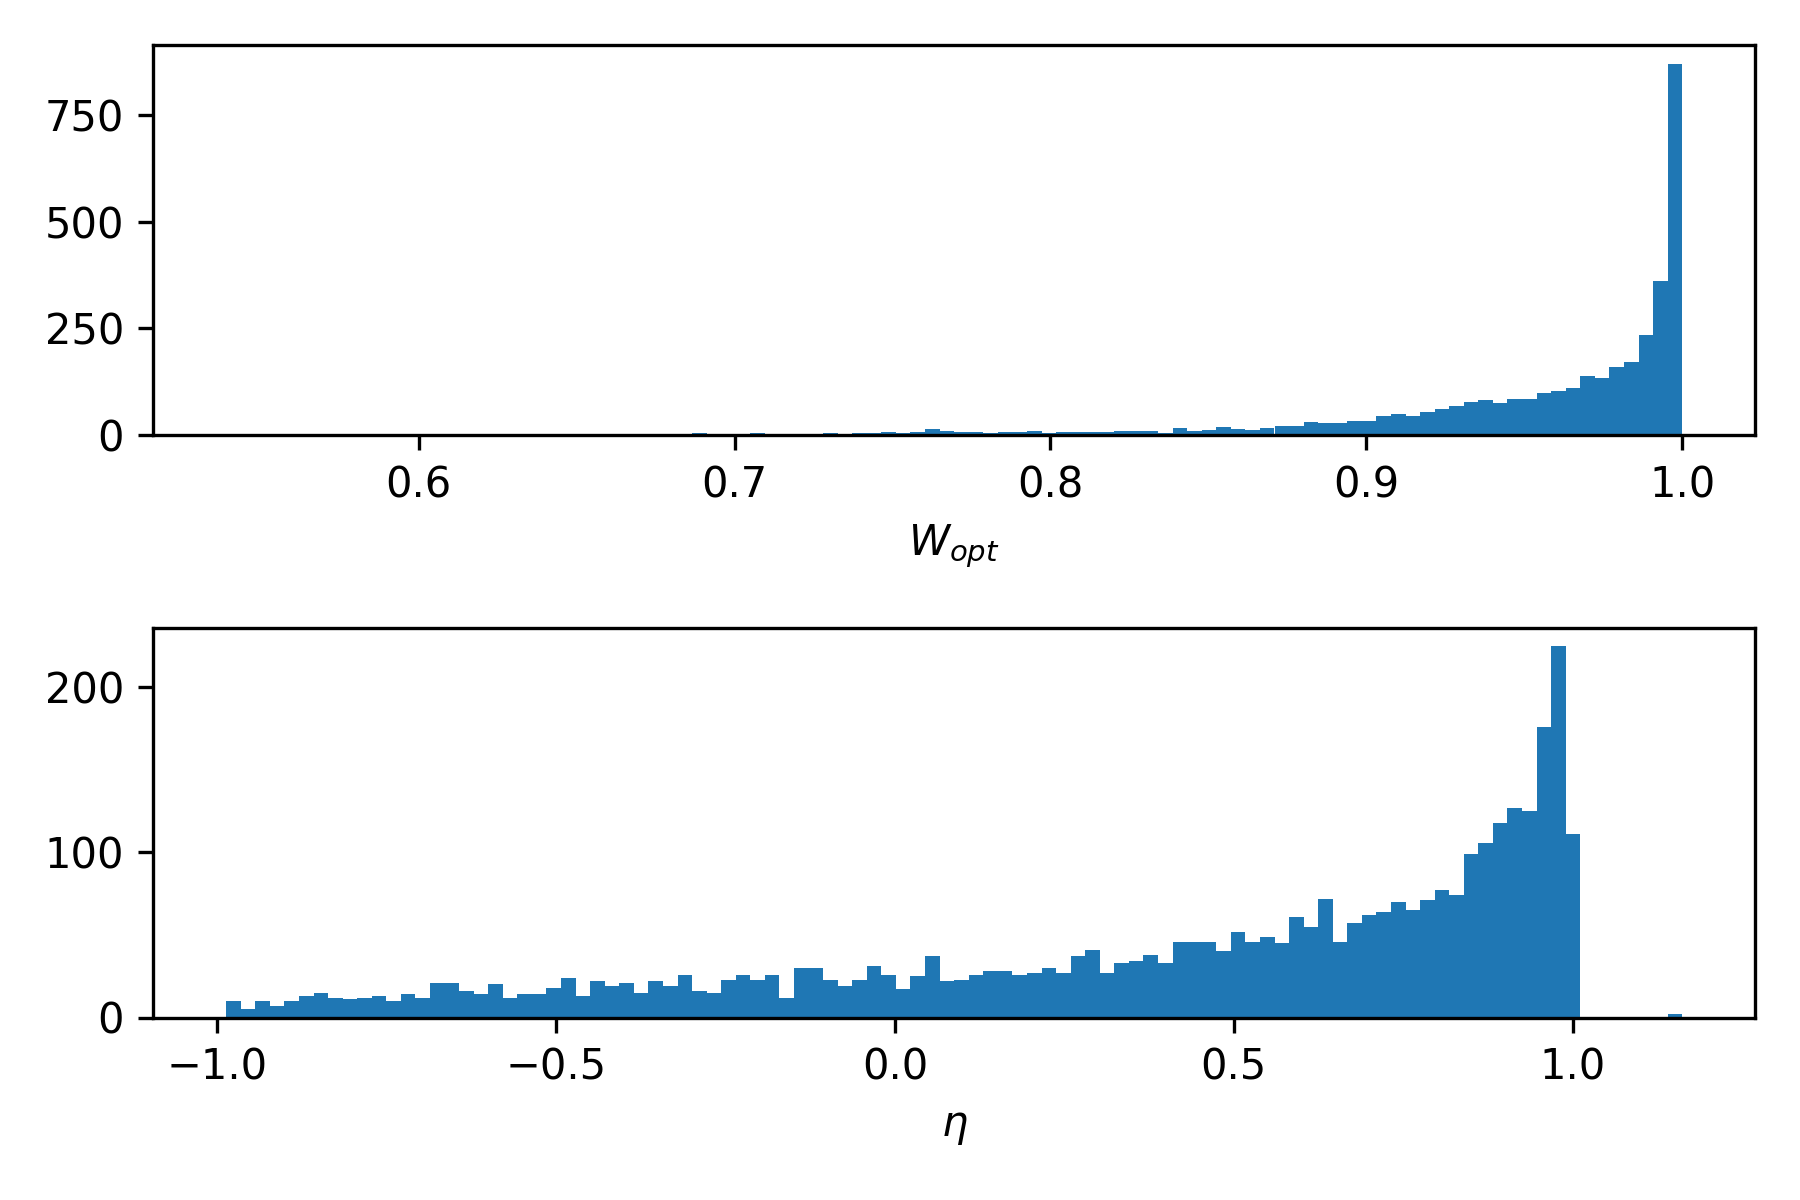
\includegraphics[width=\textwidth]{img/hist_n2_haar}
%		\caption{Random $\rho_0$}
%		\label{}
%	\end{subfigure}
%	\caption{}
%	\label{}
%\end{figure}
\section{Amount of qubit switches $N=5$}\label{n5}
\subsection{Interaction time $\Delta \mathrm{T} = 5$}\label{n_5_ml}
% !TeX root = ../BA_main_englisch.tex
% !TeX spellcheck = en_GB
In this section we examine the higher-dimensional case of $N=5$.
As the data set with $\rho_0 = \ket{+} \bra{+}$, the eigenstate of the drive Hamiltonian, performed best in the previous section, we focus our attention on this case.
We compare the efficiency of a fully connected ANN (FCANN) to a unidirectional and bidirectional LSTM to analyse the effect of different architectures on the predictive power in our setting.
Both LSTM networks have the same architecture, bar the bi-directionality (see Figure \ref{lstm_network}).
This hyperparameter distinguishes the two cases of whether or not the complete drive sequence is known in advance.
Before entering the LSTM cell, each embedded $\ket{\psi_D}$ passes through a two layer FCANN to increase the input dimensionality.
After passing the LSTM a single layer FCANN is applied to the output to produce the embedding size to recover $\ket{\psi_T}$.
The third network uses three fully connected hidden layers, the size of which is selected to approximately match the amount of trainable parameters of the bidirectional LSTM.

The test data efficiency as well as the amount of trainable parameters are presented in Table \ref{n5efftable}.

\begin{figure}
	\centering
	\includegraphics[width=0.7\textwidth]{img/lstm_network}
	\caption{Architecture of the LSTM networks. The green blocks represent the unidirectional case. For the bidirectional case, a second LSTM block (orange) is included with separate trainable parameters. The blocks labeled `FC' represent fully-connected layers.}
	\label{lstm_network}
\end{figure}

\begin{table}[h]
	\centering
	\begin{tabular}{ c | c | c | c | c}
		Network Architecture & $\eta_{test} \ [\%]$ & $\mathrm{MSE}_{test}$ & $W_{test}$ & \# Parameters \\
		\hline
		FCANN        & 19.3 & 0.1083 & 0.53 & 8,086,020 \\
		Bidir. LSTM  & 33.1 & 0.0948 & 0.91 & 7,700,222 \\
		Unidir. LSTM & 19.5 & 0.1707 & 0.52 & 3,206,990\\
	\end{tabular}
	\caption{Efficiencies $\eta$ on the test data for model architectures with given number of trainable parameters for $N=5, \ \Delta \mathrm{T} = 5$.}
	\label{n5efftable}
\end{table}

The efficiency of the best model for $N=5, \ \Delta \mathrm{T} = 5$ is drastically lower than that for $N=2$.
Crucially, the models are unable to extract the test set average of the lower bound calculated by local optimisation $W_{lo} = 1.4$.

Contrary to the case of $N=2$, the evolution of the system state becomes relevant over multiple time steps.
As the work per time step is determined by $\mathrm{dW} = -\Tr{\rho_S \ dH} = \Tr{\rho_S (H_{ST}^i - H_{ST}^{i+1})}$, finding the optimal solution is a compromise of choosing $dH$ so as to maximise the expectation value while controlling the unitary evolution of $\rho_S$ such that $\Tr{\sigma_z \rho_S}$ is small.
We plot the optimal and predicted trajectory of a random data point in the test in Figure \ref{bloch_10553} set to illustrate this compromise.
In \ref{bloch_worst} we plot the trajectories for the worst-performing sample in the test set.
In this case, the prediction for $\ket{\psi_T}$ deviates only slightly from the optimum for $i \in [2, N]$ but deviates significantly for $i=1$.
This illustrates the problem of using the MSE as a cost function for training - to the network, this is a good prediction as most transducer qubits are near their optimal setting.
The deviation in the first qubit causes a completely different evolution on the system, especially as $\Delta \mathrm{T} = 5$ is large.
This leads to a negative work output when following the predicted protocol.


\begin{figure}
	\centering
	\begin{subfigure}{0.85\textwidth}
		\centering
		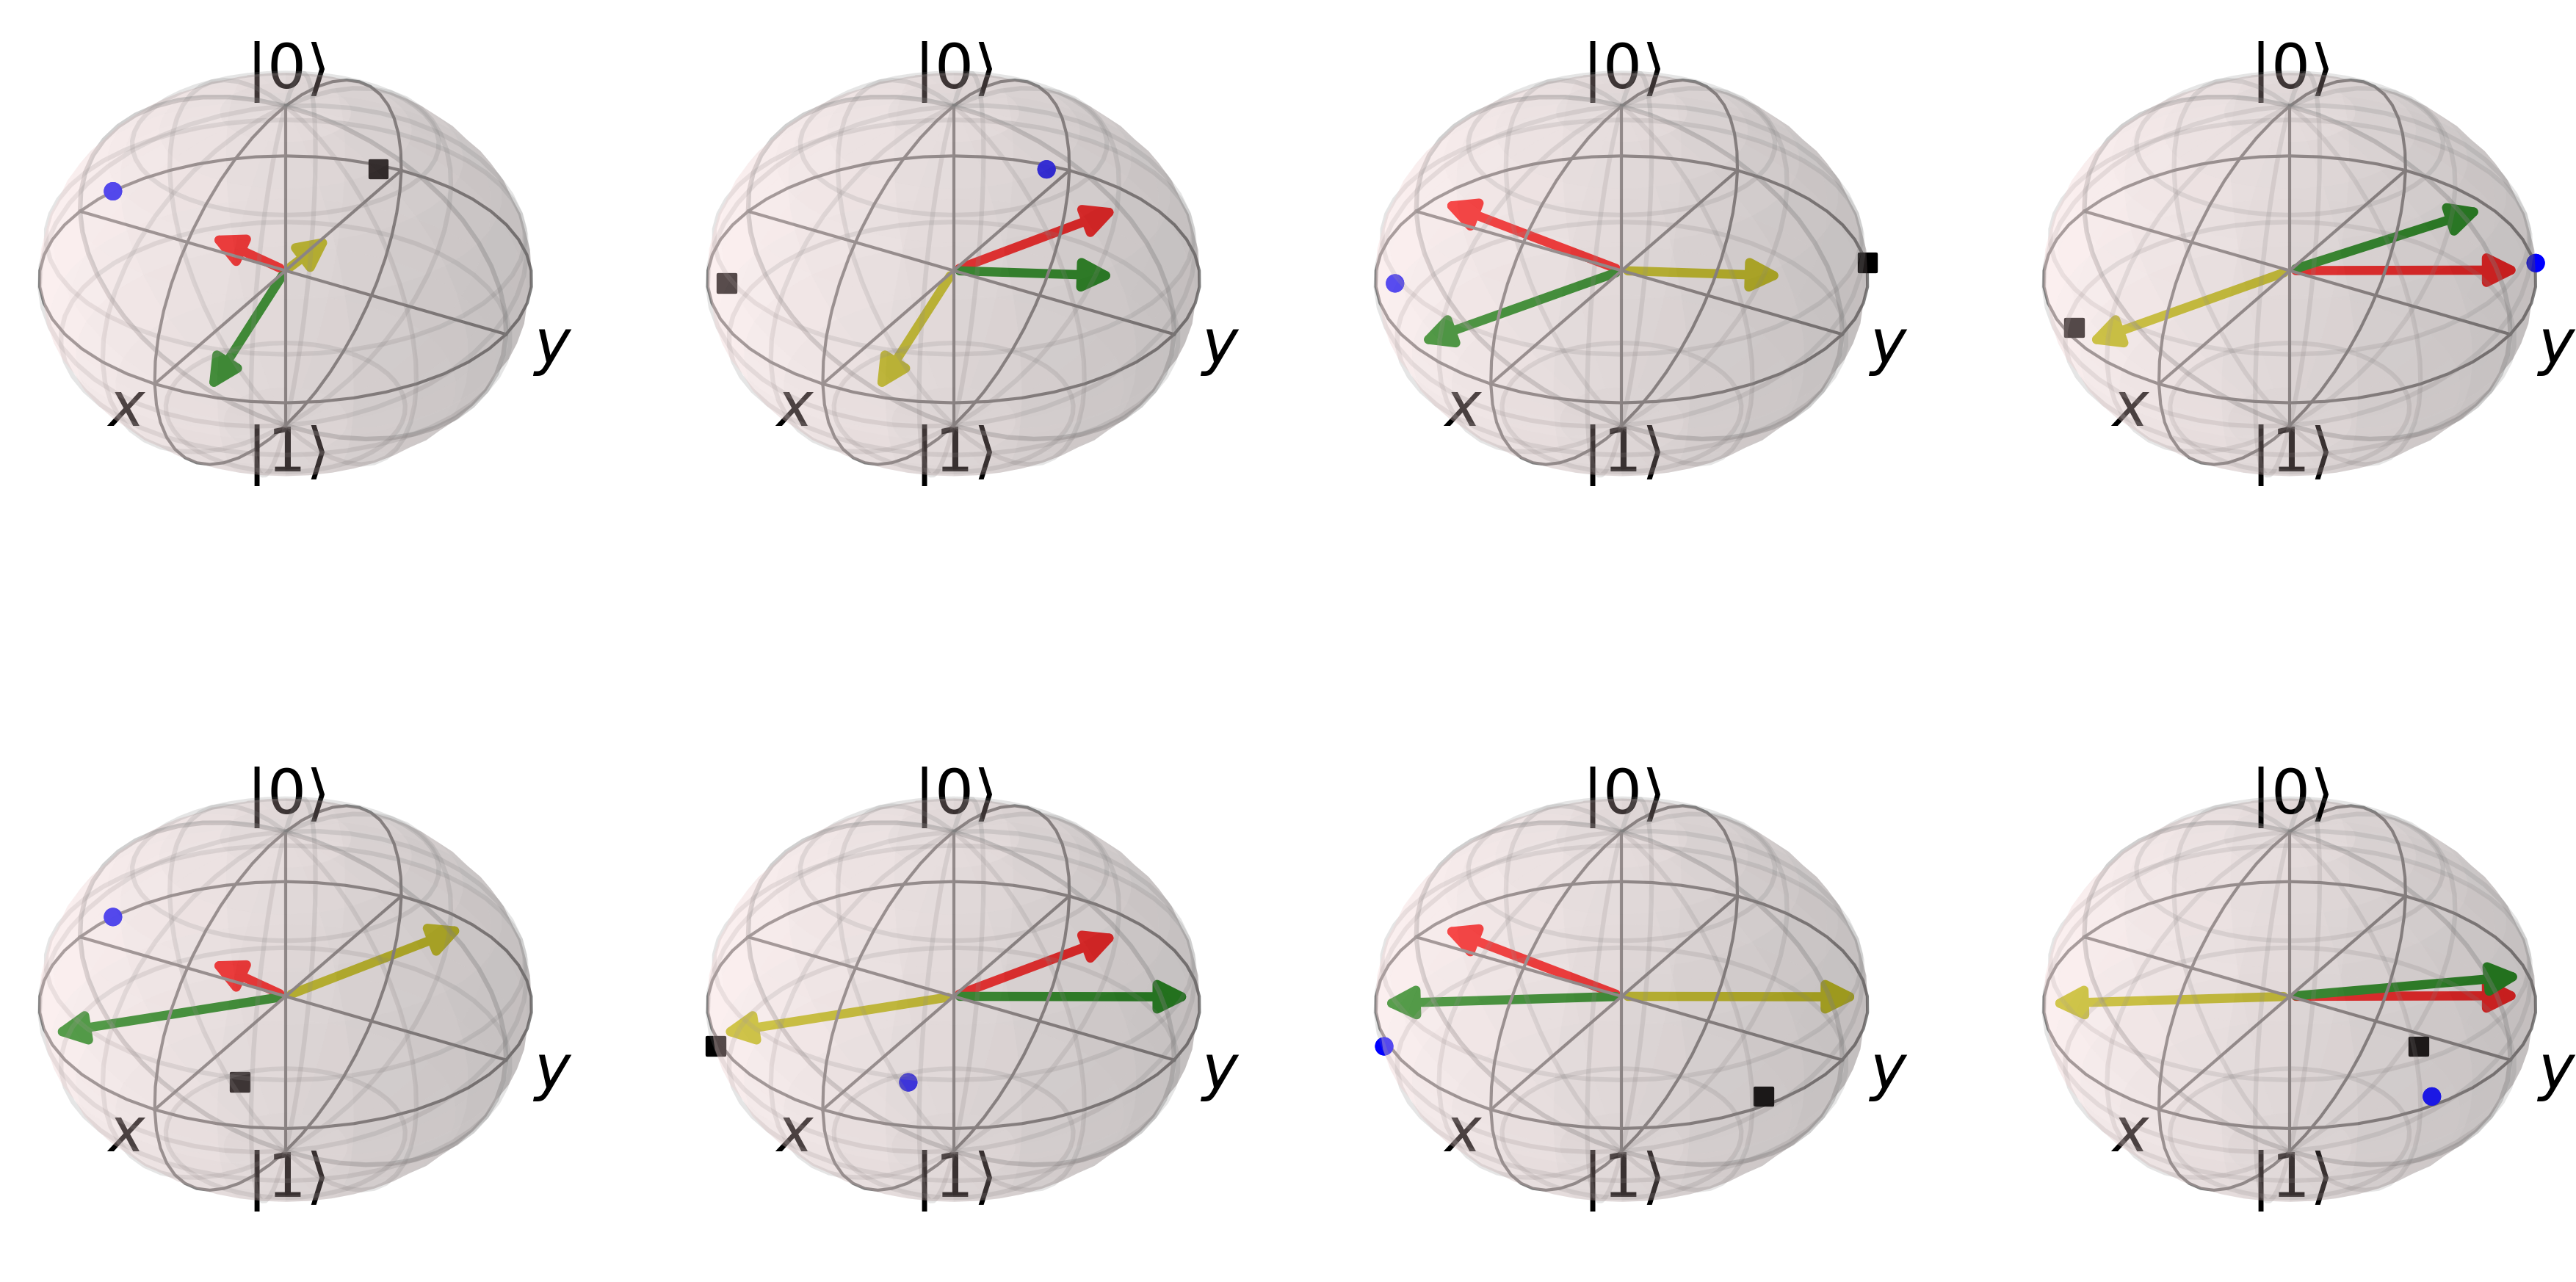
\includegraphics[width=\textwidth]{img/bloch_10553_crop}
		\caption{$W_{opt} = 3.03, W_{pred} = 1.11$}
		\label{bloch_10553}
	\end{subfigure}
	\begin{subfigure}{0.85\textwidth}
		\centering
		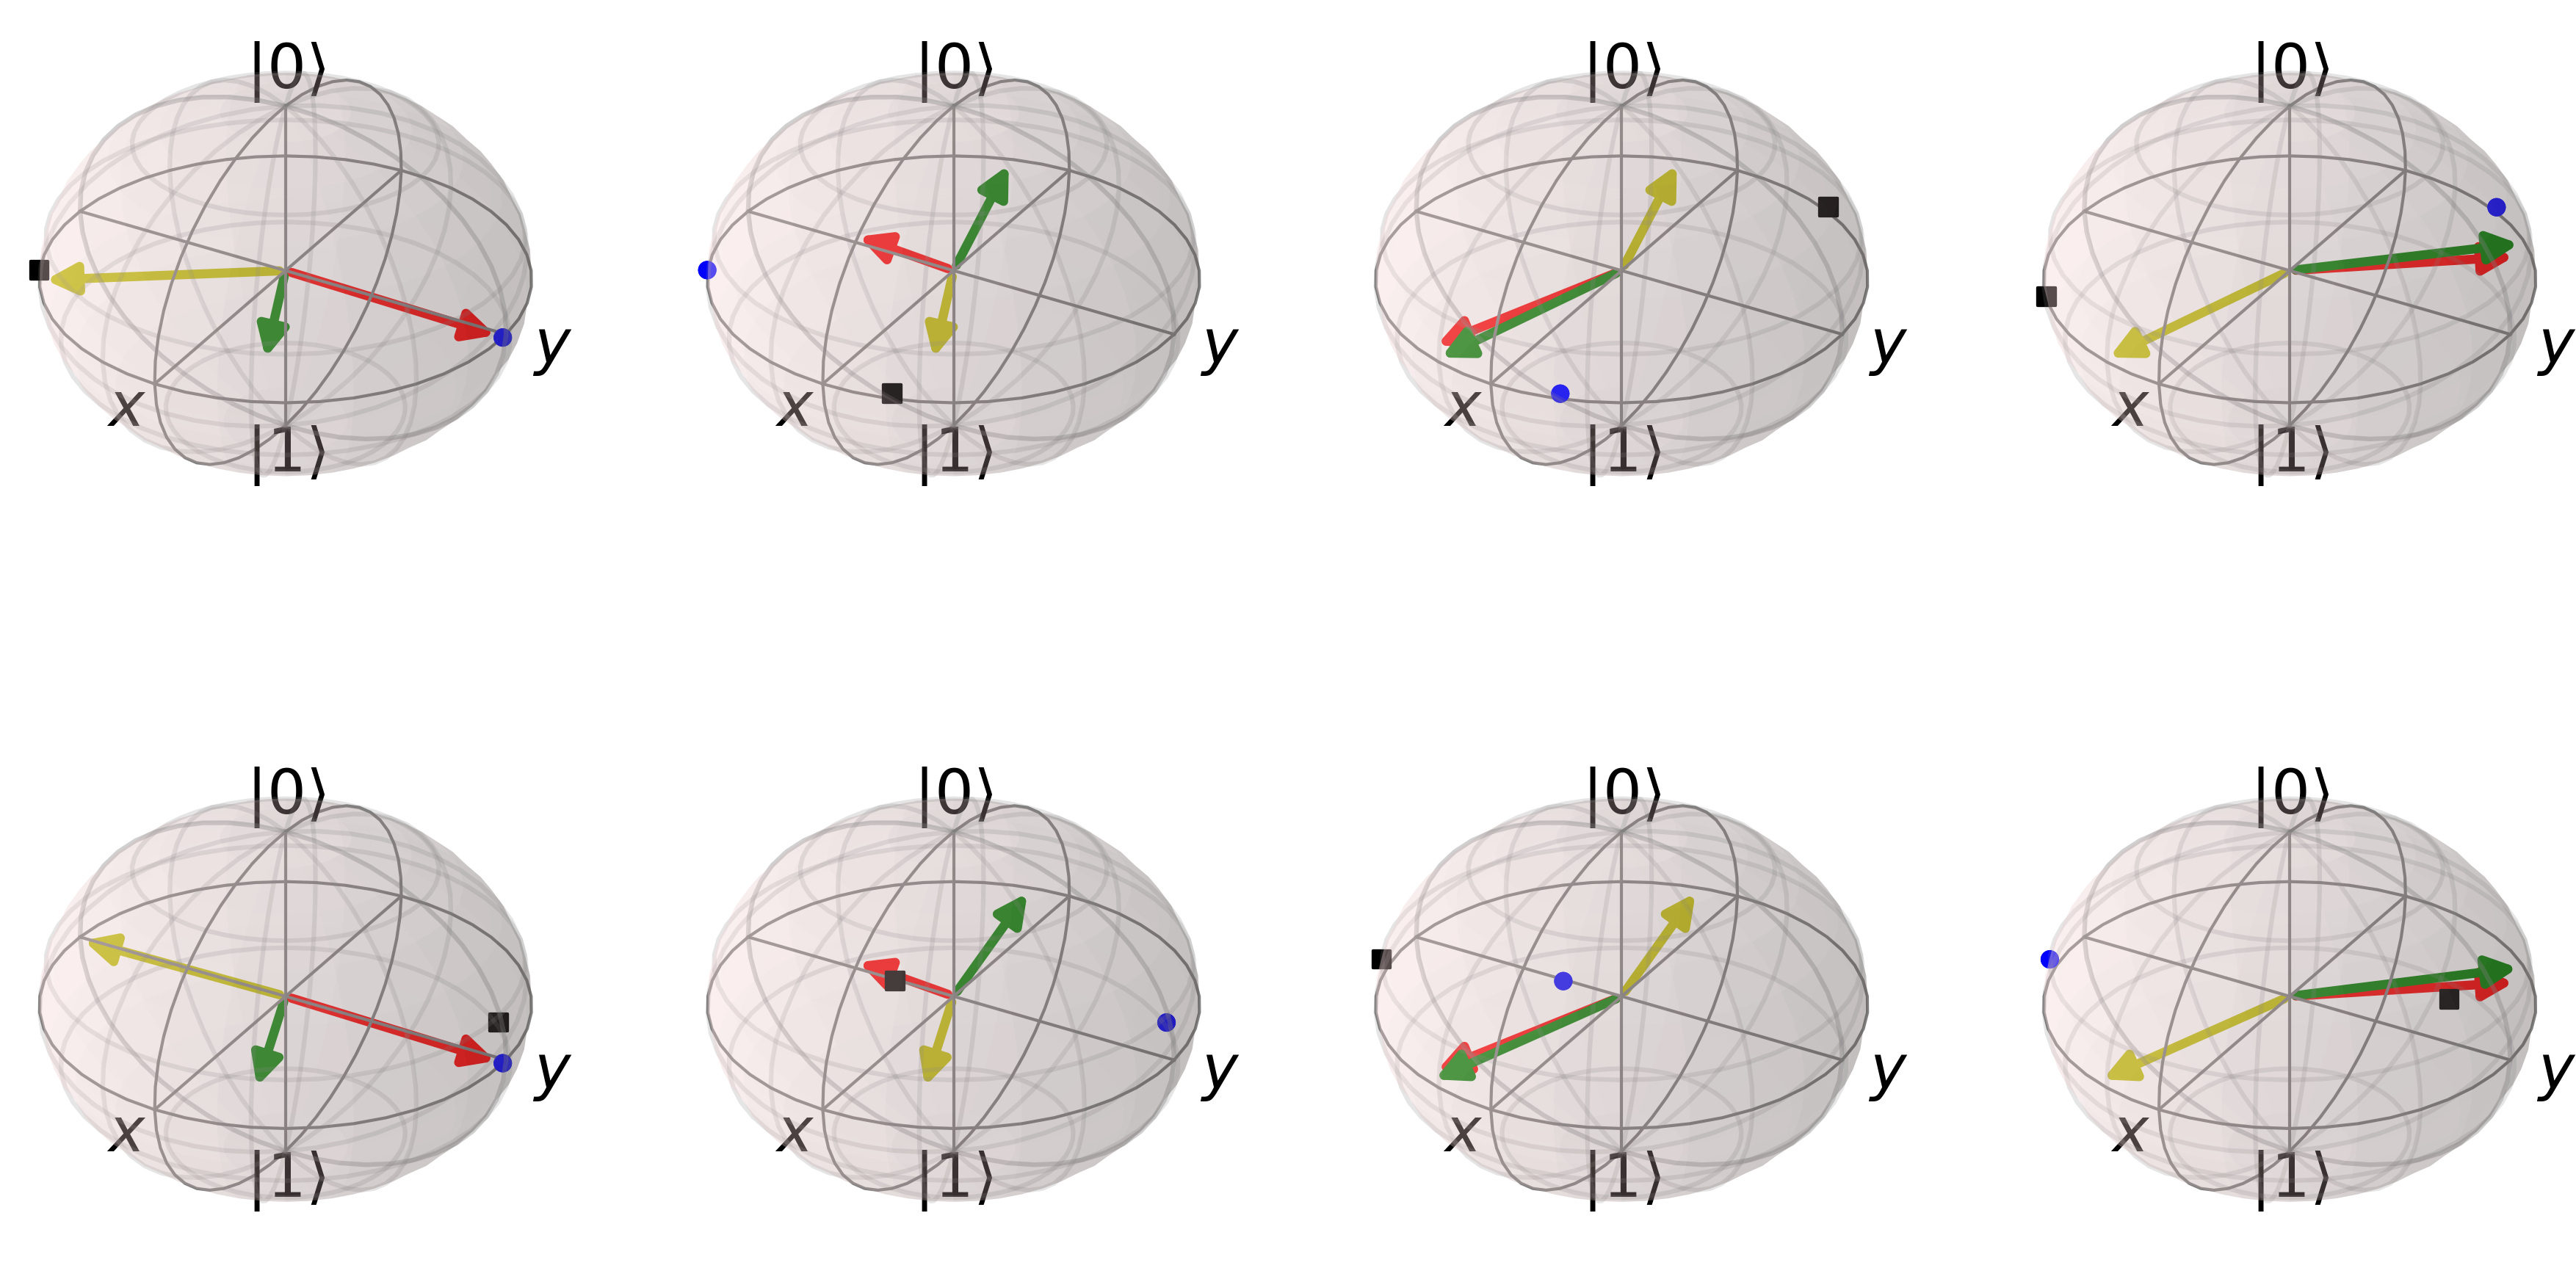
\includegraphics[width=\textwidth]{img/bloch_worst_crop}
		\caption{$W_{opt} = 3.06, W_{pred} = -2.65$}
		\label{bloch_worst}
	\end{subfigure}
	\caption{\textbf{(a)} We plot the evolution of a single sample from the test set for $N=5$ and $\Delta \mathrm{T} = 5$. For this sample we have $W_{opt} = 3.03, W_{pred} = 1.11$. Each Bloch sphere shows $\rho_S^i$ (blue dot), $\rho_S^{i+1}$ (black square), the partial system Hamiltonian acting only between system and drive $H_{DS}^i$ (red vector) as well as $H_{ST}^i$ (yellow vector) and $H_{ST}^{i+1}$ (green vector). \textbf{Top row:} we plot the system dynamics for the transducer series generated by the optimiser for $i \in [1, N - 1]$. In the optimal case, $H_{ST}^i$ is chosen such that $\rho_S$ remains near the x-y-plane for all times and $\Tr{\rho_S^{i+1} H_{DS}^i}$ is large. \textbf{Bottom row:} we plot the dynamics for the same drive protocol with transducer qubits predicted by the bidirectional LSTM. The overall difference of $\rho_S$ to the x-y-plane is larger. As shown in Figure \ref{bilstmbox}, $\theta_T$ is often set to $\frac{\pi}{2}$ which maximises the strength of $H_{ST}$ as can be seen in all Bloch spheres in the bottom row. In this case, the $H_{DS}$ are chosen by the network to be antiparallel, irrespective of the current system state.
	\textbf{(b)} We show the same plot as in (a) for the worst performing sample from the test set to illustrate a shortcoming of the model. As can be seen from the yellow and green vectors, the predictions for $j \in [2, N]$ are very close to the optimal solutions. However, the first transducer prediction is wrong, leading to a deviation from the optimal system dynamics.}
	\label{n_5_blochs}
\end{figure}

Figure \ref{bilstmbox} shows the prediction of the bidirectional LSTM and optimal values for the trajecto-ries of each data point in the test set.
There is a notable difference in the predictive quality between the first four qubits and the last one: for the final qubit the dynamics after the work extraction step are inconsequential.
It is therefore beneficial to maximise the strength during the final switching, i.e. setting $\theta_T^N = \frac{\pi}{2}$, to maximise its work output.
Additionally $\phi_T^N$ is should be set so that $H_{ST}^N$ is antiparallel to $\rho_S^N$ on the Bloch sphere.

\begin{figure}
	\centering
	\begin{subfigure}{0.32\textwidth}
		\centering
		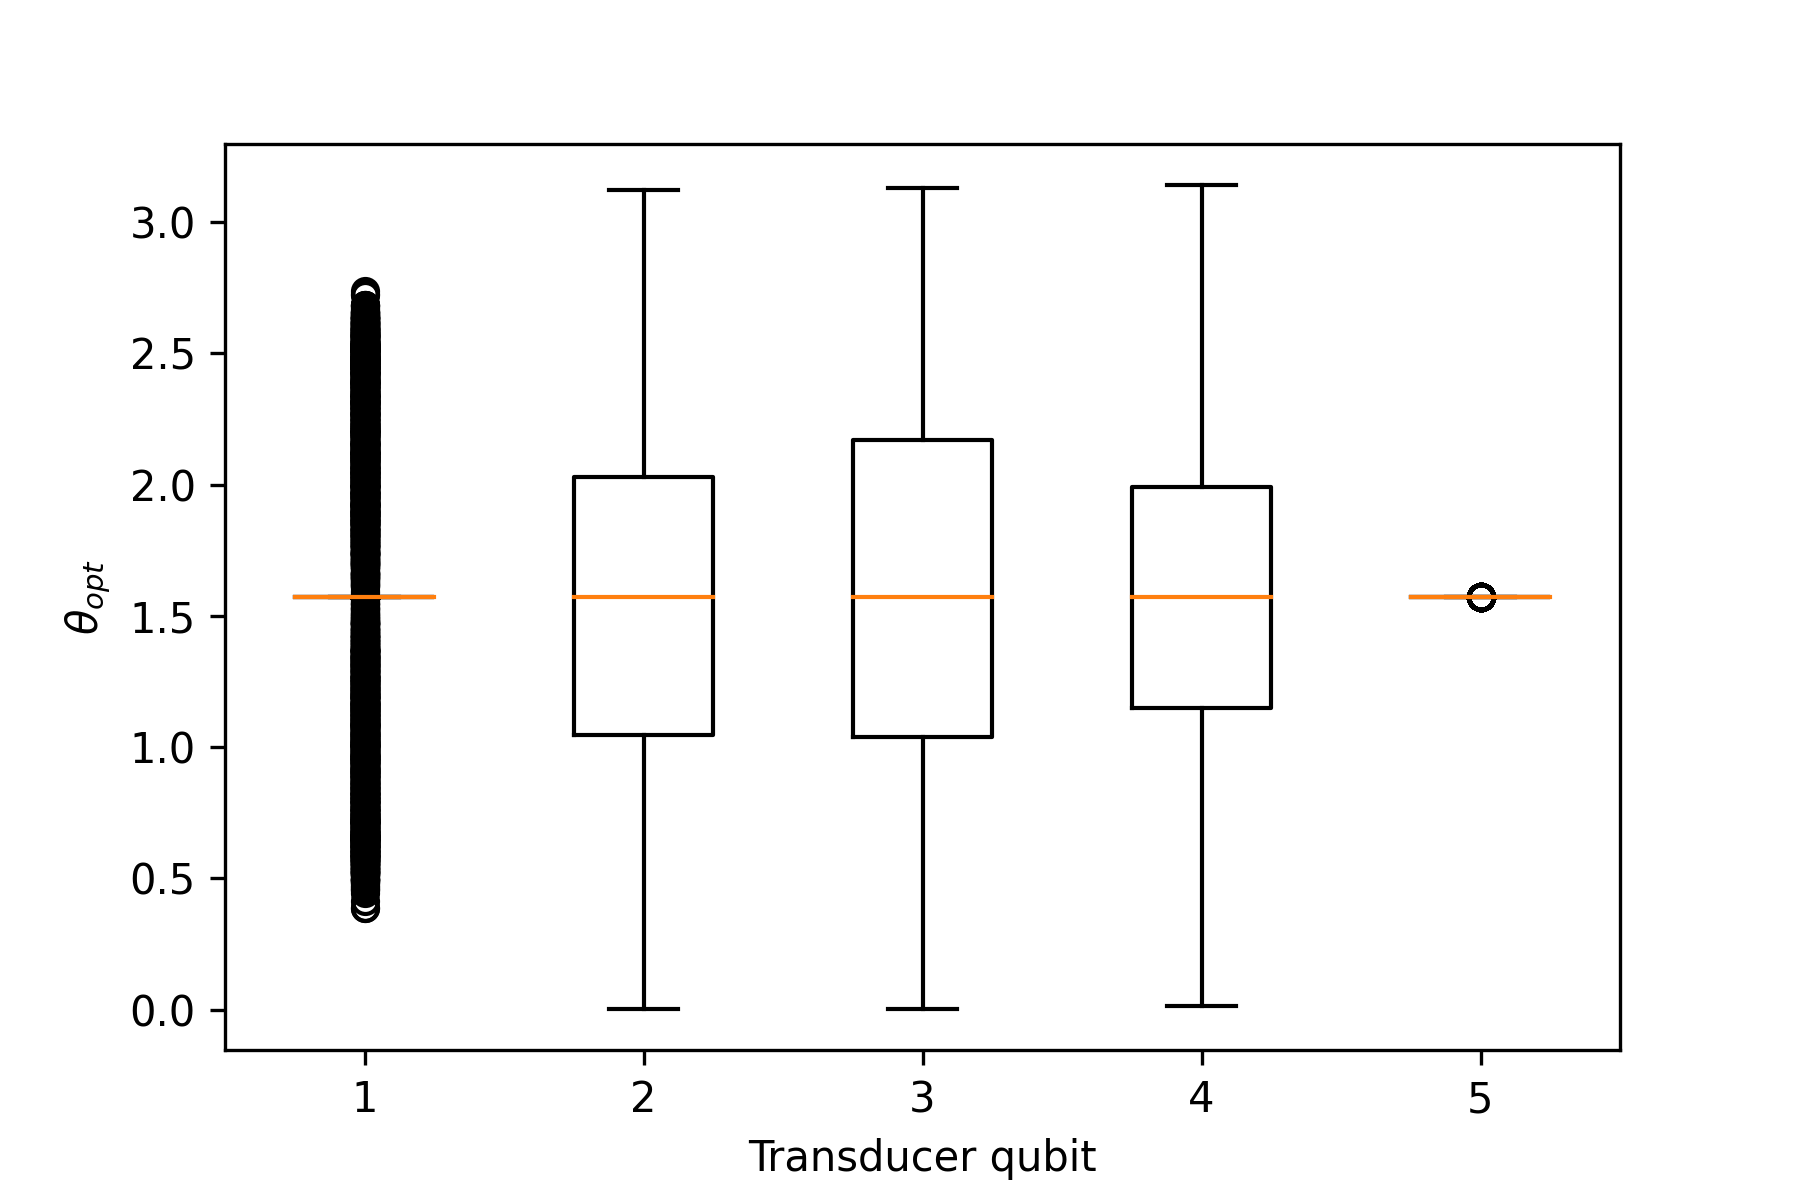
\includegraphics[width=\textwidth]{img/theta_opt_box}
	\end{subfigure}
	\begin{subfigure}{0.32\textwidth}
		\centering
		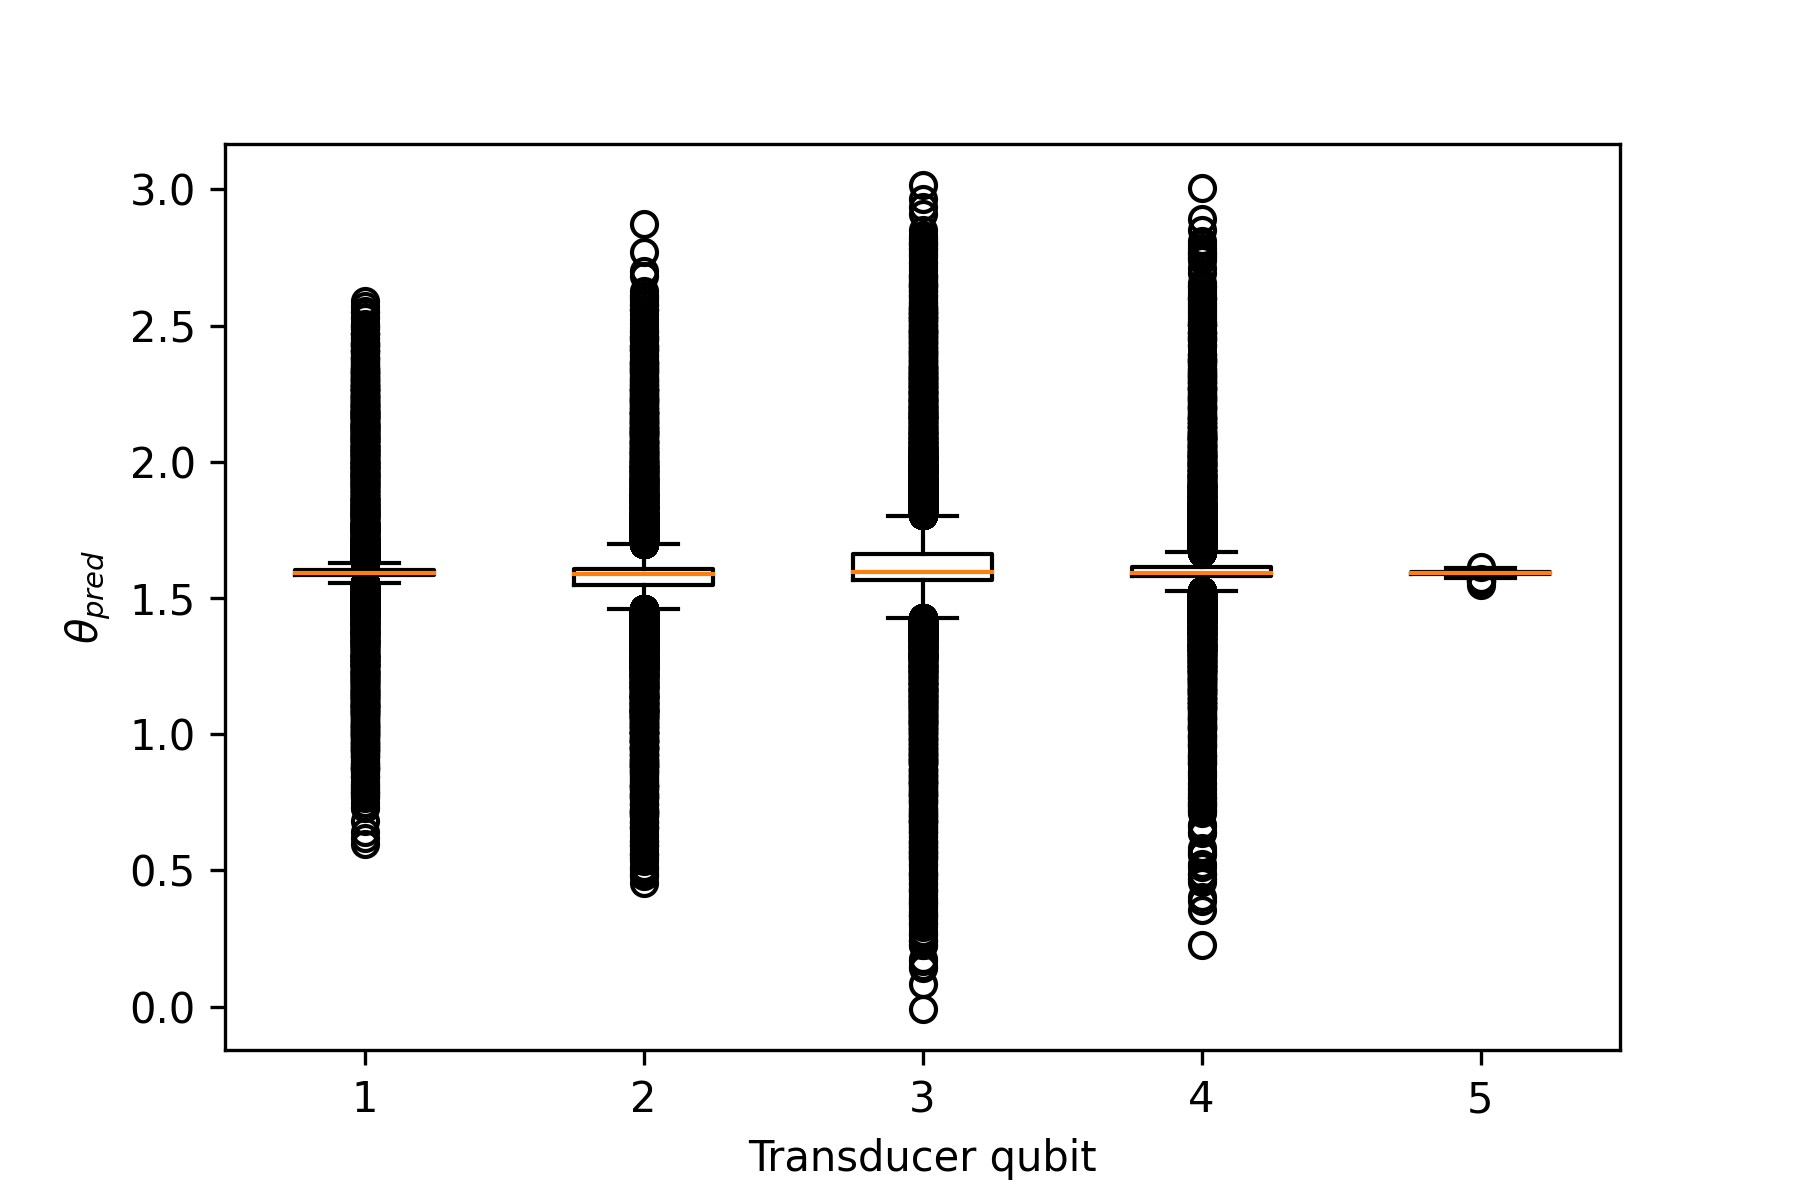
\includegraphics[width=\textwidth]{img/theta_pred_box}
	\end{subfigure}
	\begin{subfigure}{0.32\textwidth}
		\centering
		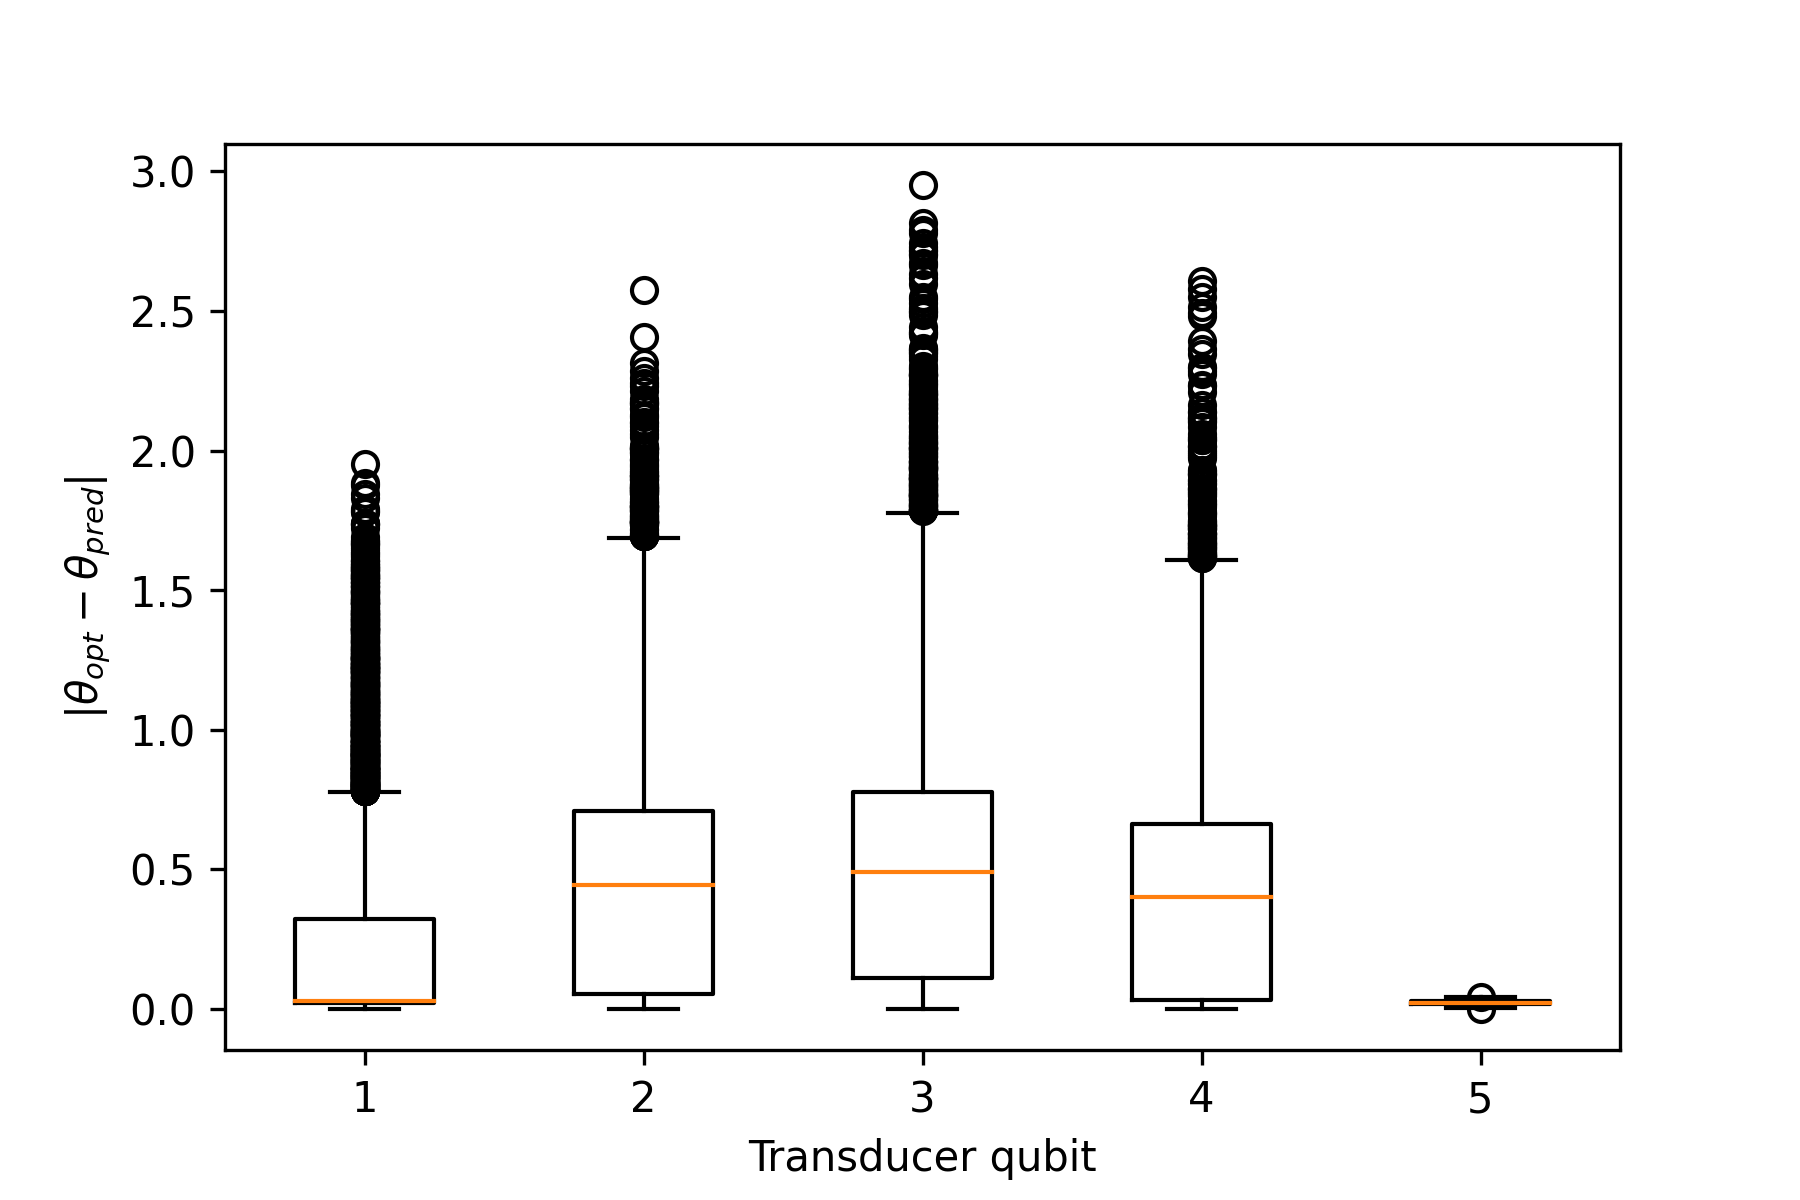
\includegraphics[width=\textwidth]{img/delta_theta_box}
	\end{subfigure}
	\begin{subfigure}{0.32\textwidth}
	\centering
	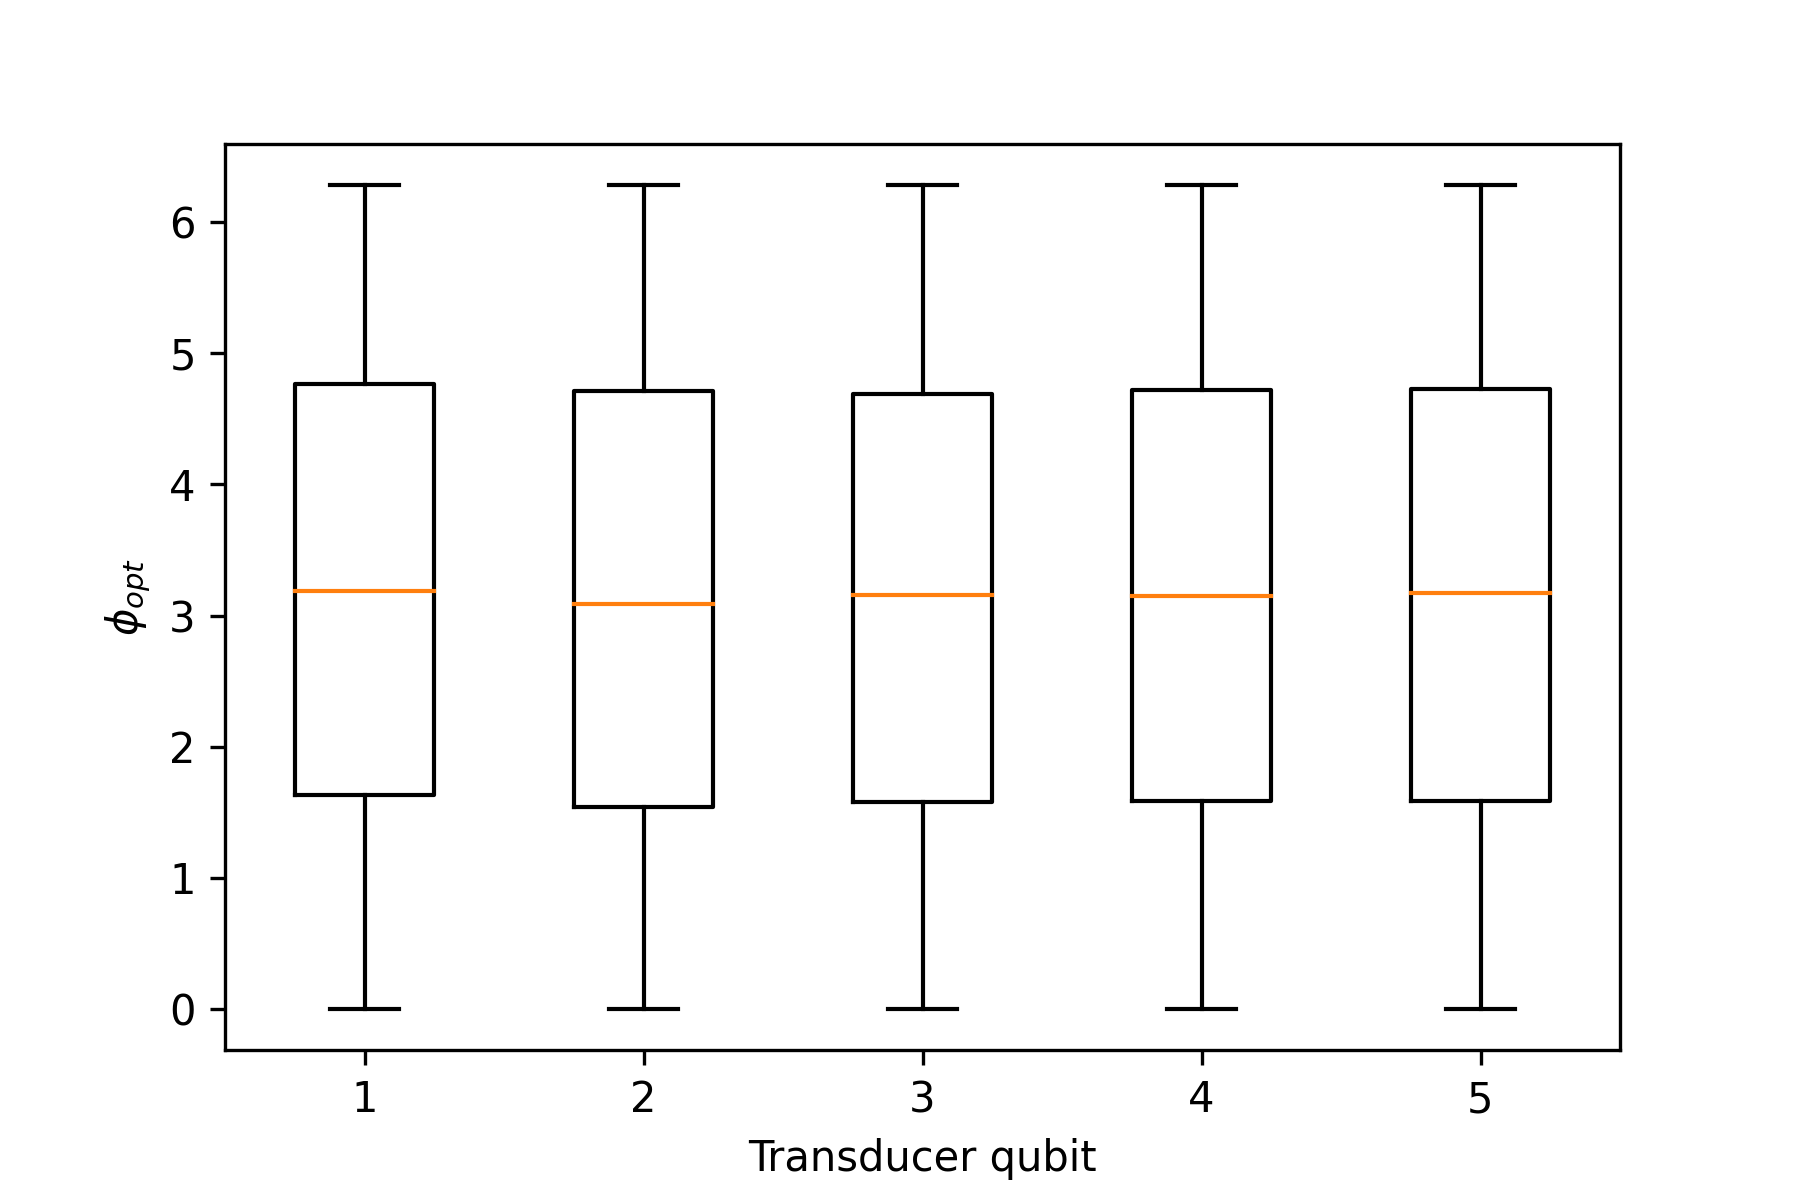
\includegraphics[width=\textwidth]{img/phi_opt_box}
\end{subfigure}
\begin{subfigure}{0.32\textwidth}
	\centering
	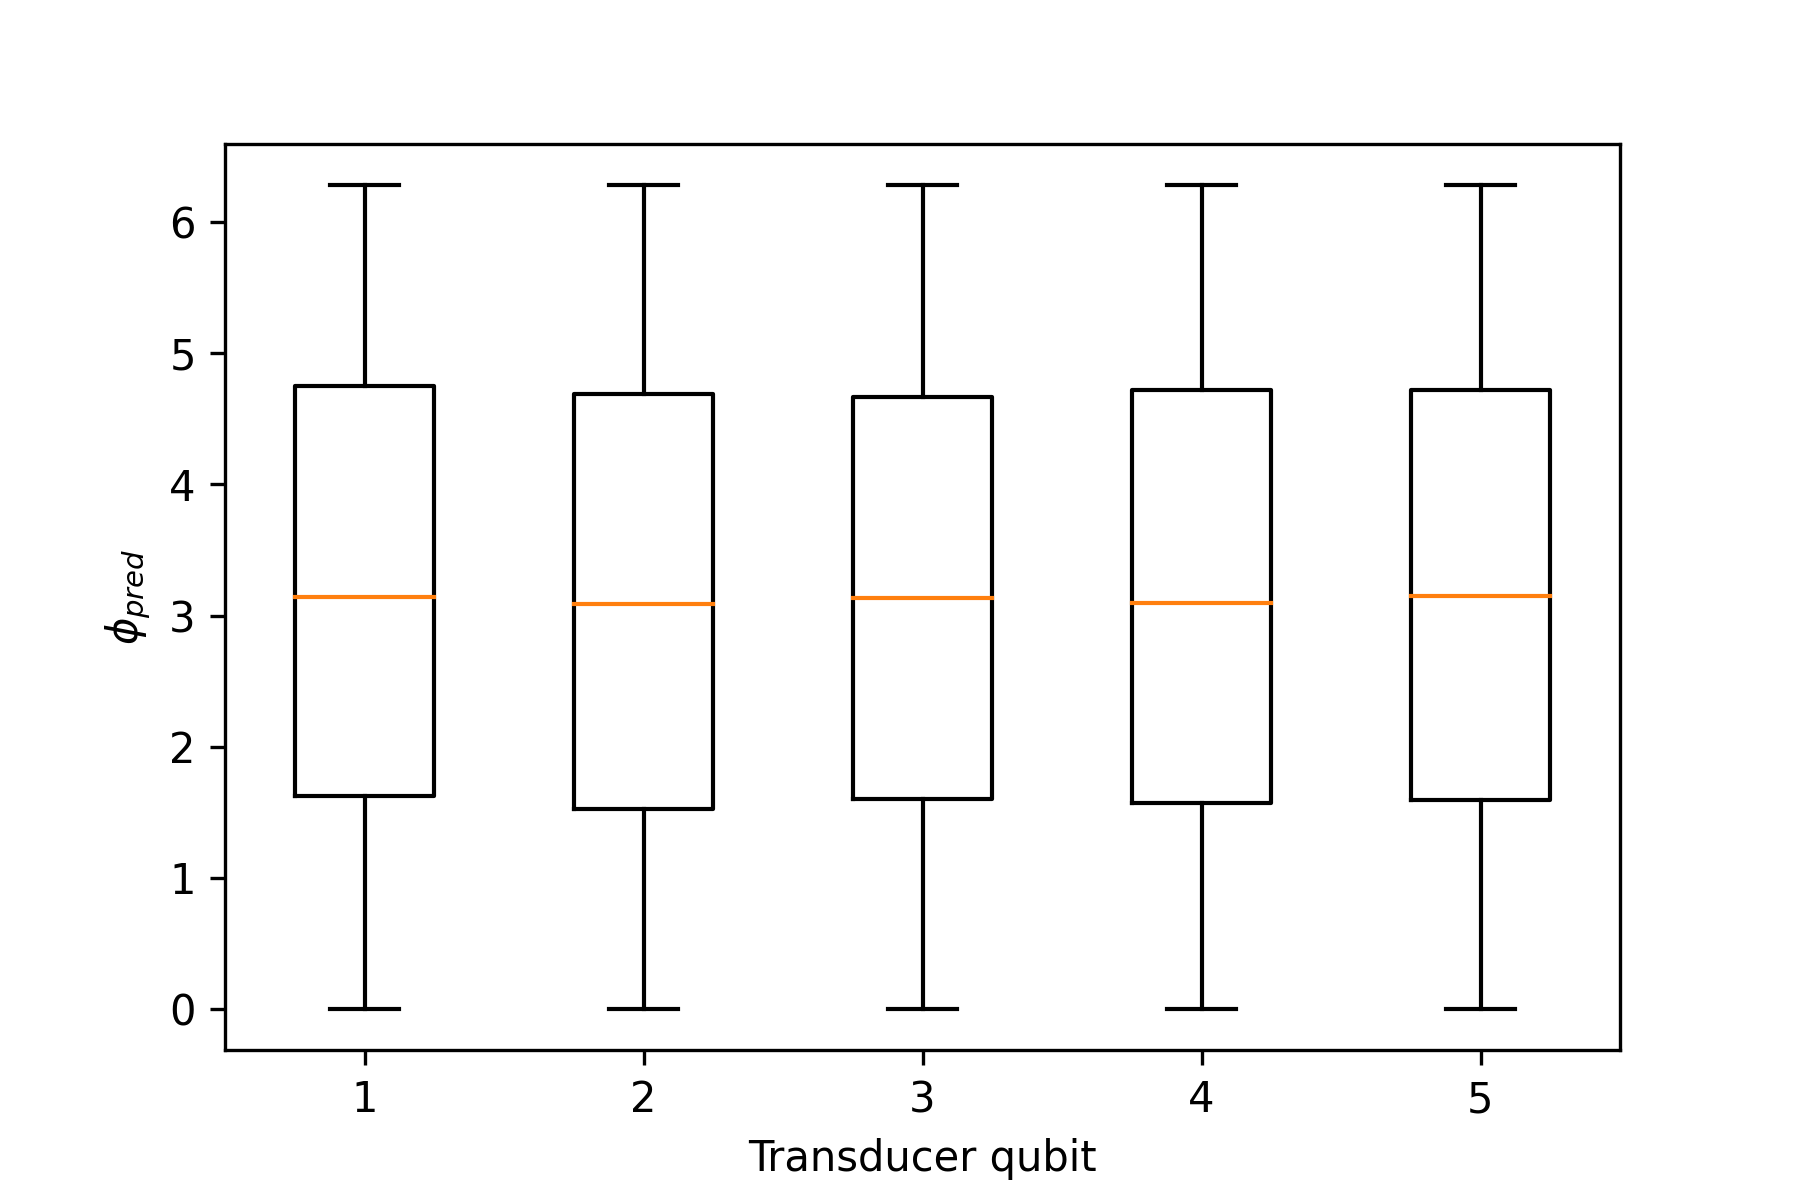
\includegraphics[width=\textwidth]{img/phi_pred_box}
\end{subfigure}
\begin{subfigure}{0.32\textwidth}
	\centering
	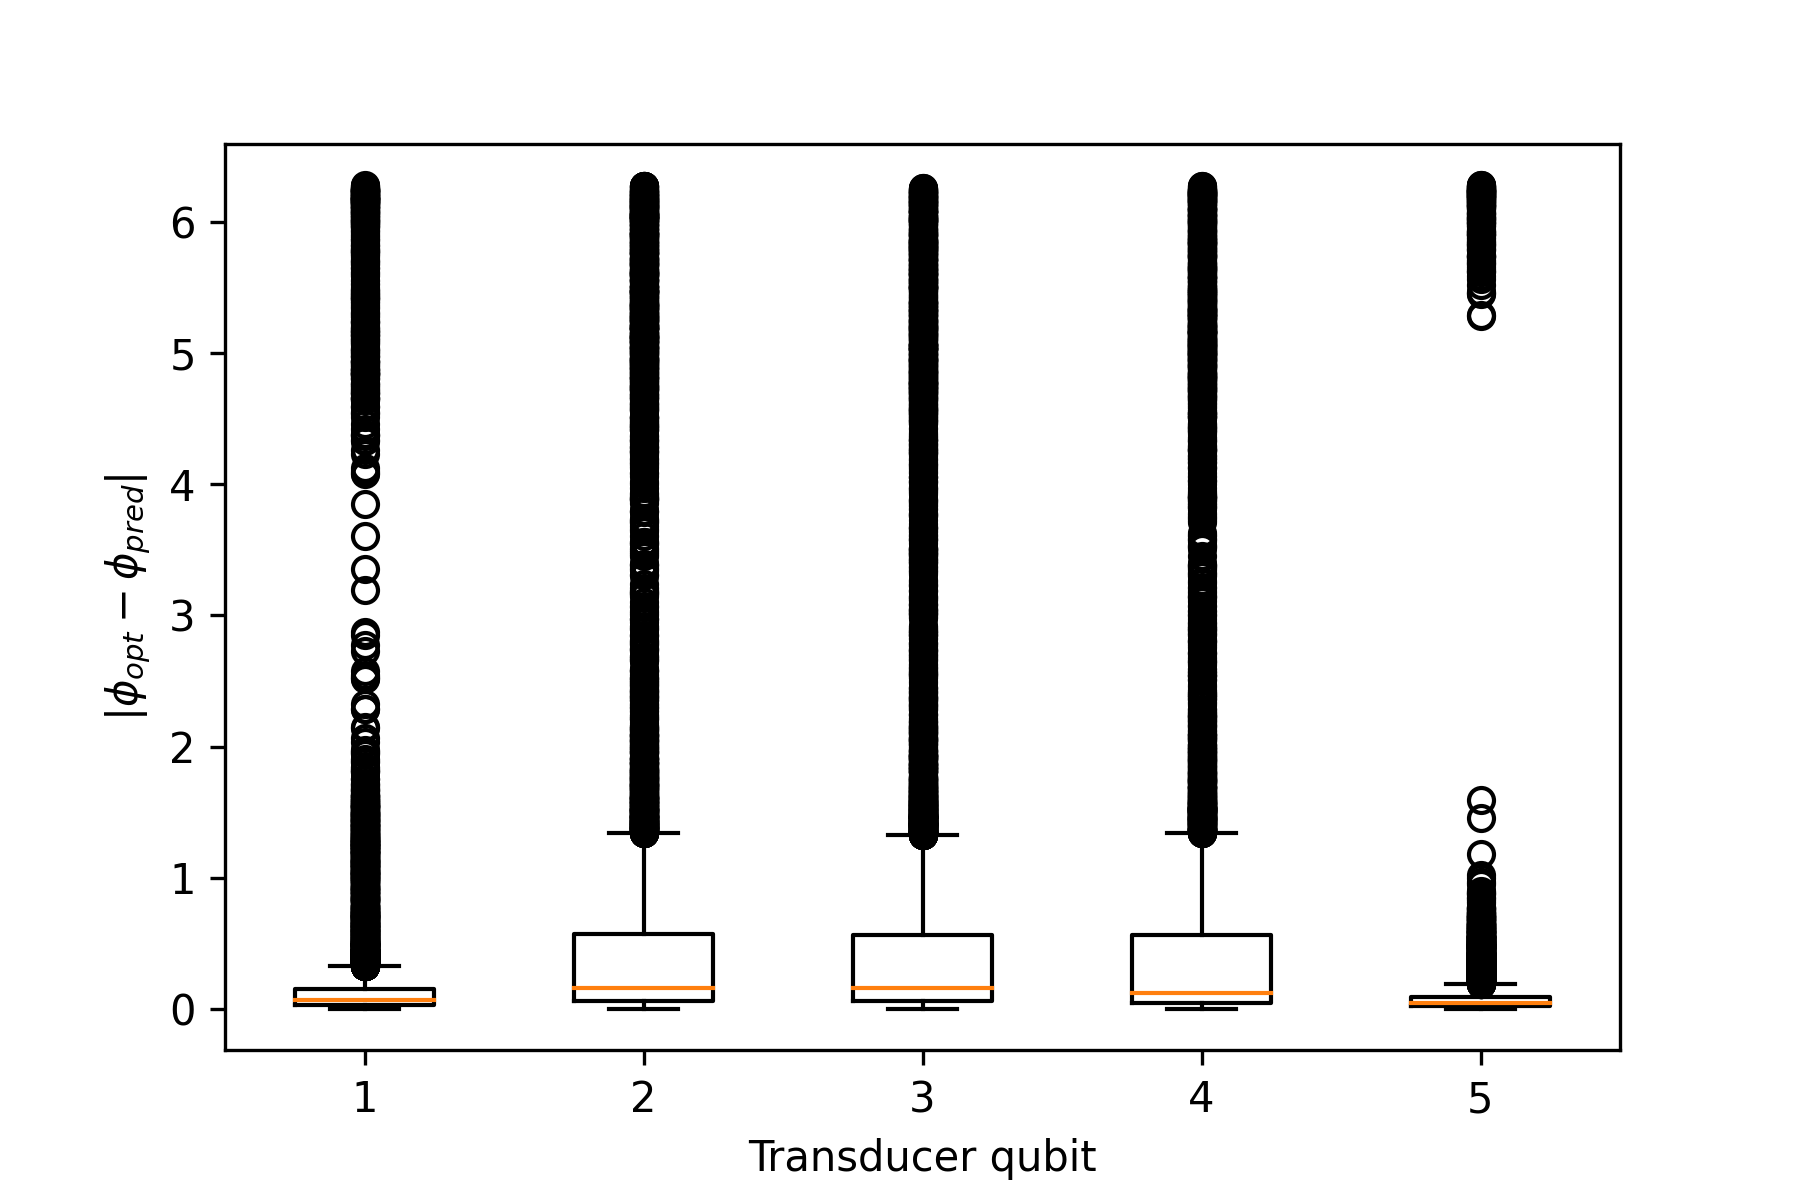
\includegraphics[width=\textwidth]{img/delta_phi_box}
\end{subfigure}
\caption{\textbf{Top row:} for the bidirectional LSTM network and $\Delta \mathrm{T} = 5$, we plot boxplots of the optimal, predicted and absolute differences of $\theta_T$ for the five qubits of each trajectory in the test set. The prediction for $\theta_T^N$ is very good as the optimal solution is to set it to $\frac{\pi}{2}$ in all cases to maximise the work output of the final step. The prediction for $\theta_T^0$ is reasonably good too, as the optimal solution is again $\frac{\pi}{2}$ in a majority of trajectories. The network is unable to predict the three central qubits, with median absolute differences of approximately $0.5$. \textbf{Bottom row:} we plot the same quantities as above for the transducer azimuth $\phi_T$.}
\label{bilstmbox}
\end{figure}

\subsection{Interaction time $\Delta \mathrm{T} = 1$}\label{n_5_dt1}
% !TeX root = ../BA_main_englisch.tex
% !TeX spellcheck = en_GB
We apply the methodology of Section \ref{n_5_ml} to the case of $\Delta \mathrm{T} = 1$ with 5 Drive and Transducer qubits.
Contrary to $\Delta \mathrm{T} = 5$, the optimal system states\footnote{$\Tr{\rho_S^i \sigma_z} = 0$} cannot be reached from every point on the Bloch sphere, leading to a lower total work output following the protocol determined by the optimiser (Figure \ref{dt_dep}).

We train the LSTM networks from Section \ref{n_5_ml} as well a network with a larger cell state dimension to match the amount of trainable parameters of the bidirectional LSTM.
The performance of each network is listed in Table \ref{effdt1}.
We find that all networks perform better than their $\Delta \mathrm{T} = 5$ counterparts, both in terms of efficiency and average work output.
In addition, the MSE score on the test data is lower, indicating that the predictions themselves are better.
There are two reasons for this occurrence: firstly, the predictive power of the networks is greater for $\Delta \mathrm{T} = 1$ than $\Delta \mathrm{T} = 5$, illustrated in Figure \ref{dt1box}.
Secondly, deviations between optimal and predicted Transducer settings lead to a smaller difference between the respective system states as the evolution time is shorter.

\begin{figure}
	\centering
	\begin{subfigure}{0.32\textwidth}
		\centering
		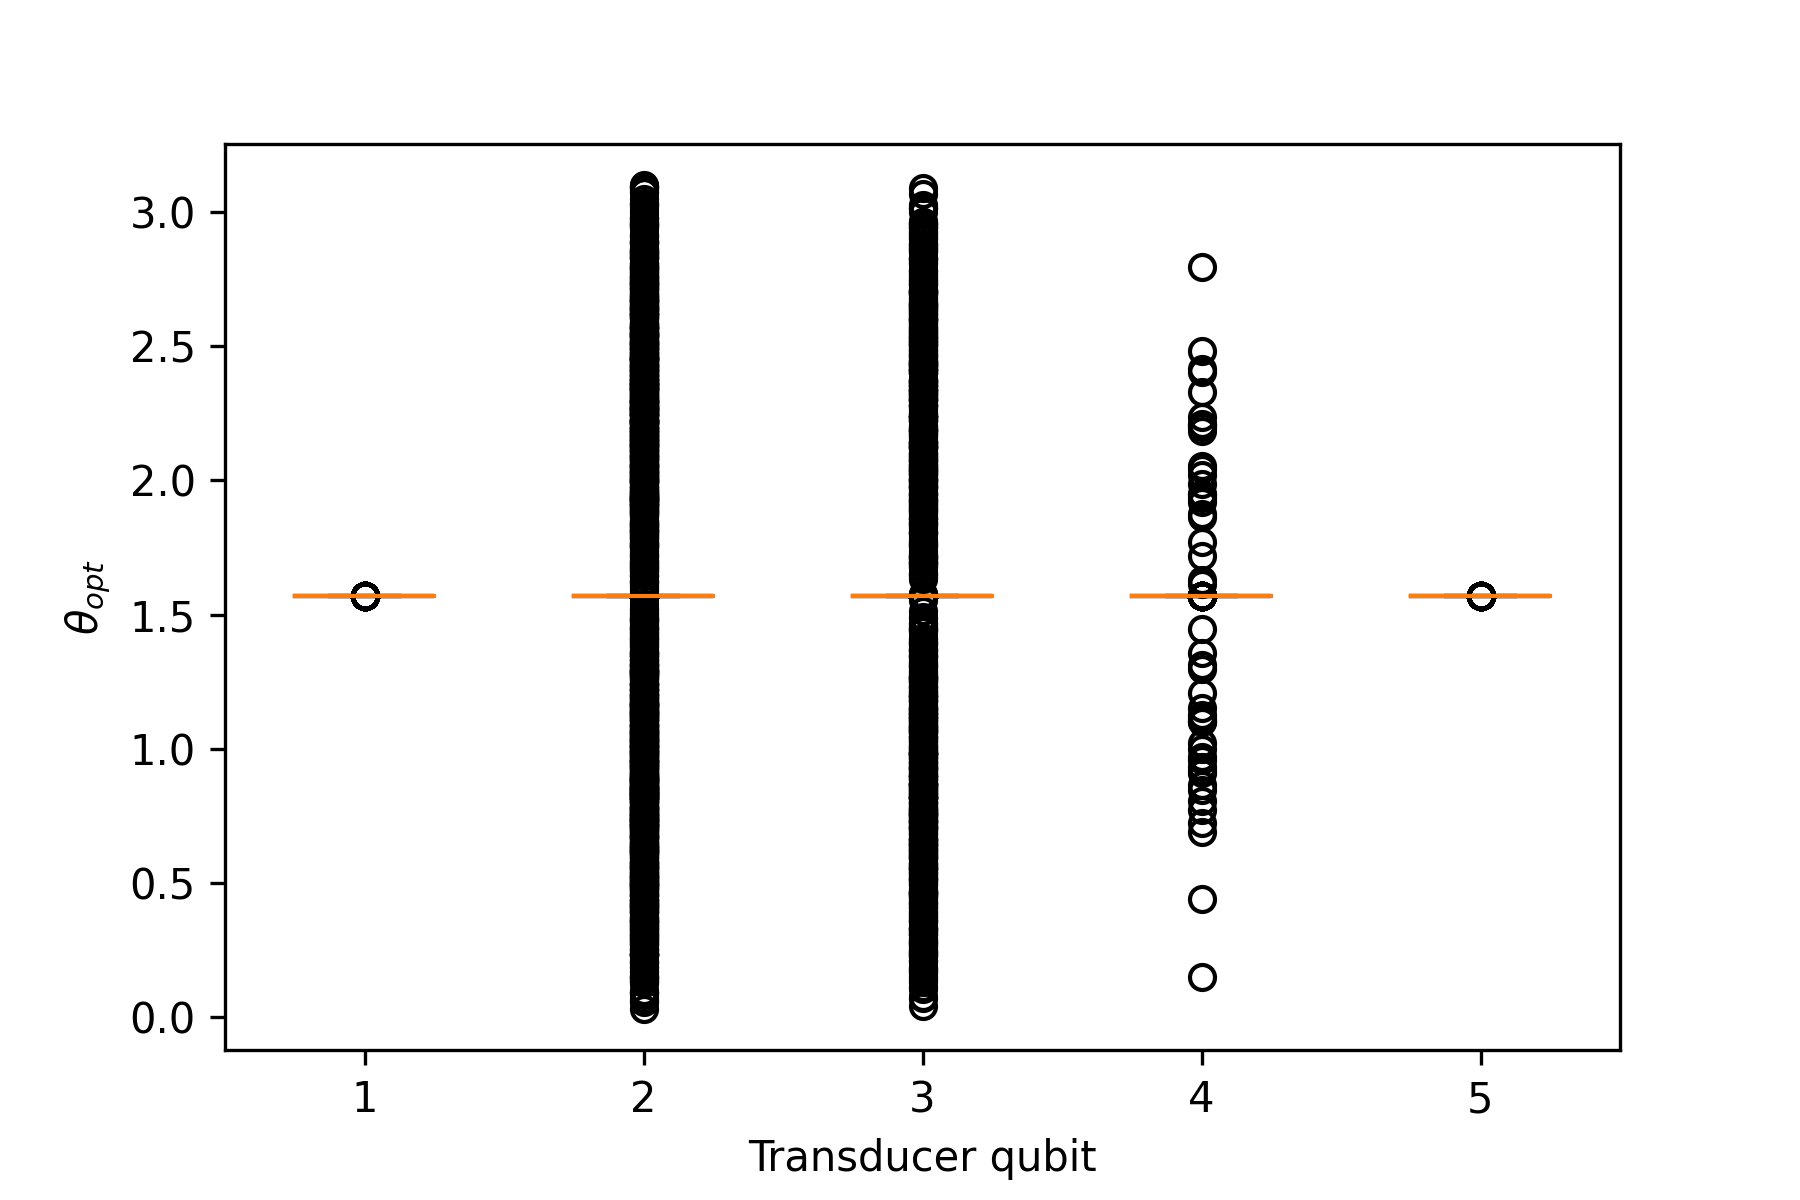
\includegraphics[width=\textwidth]{img/theta_opt_box_dt_1}
	\end{subfigure}
	\begin{subfigure}{0.32\textwidth}
		\centering
		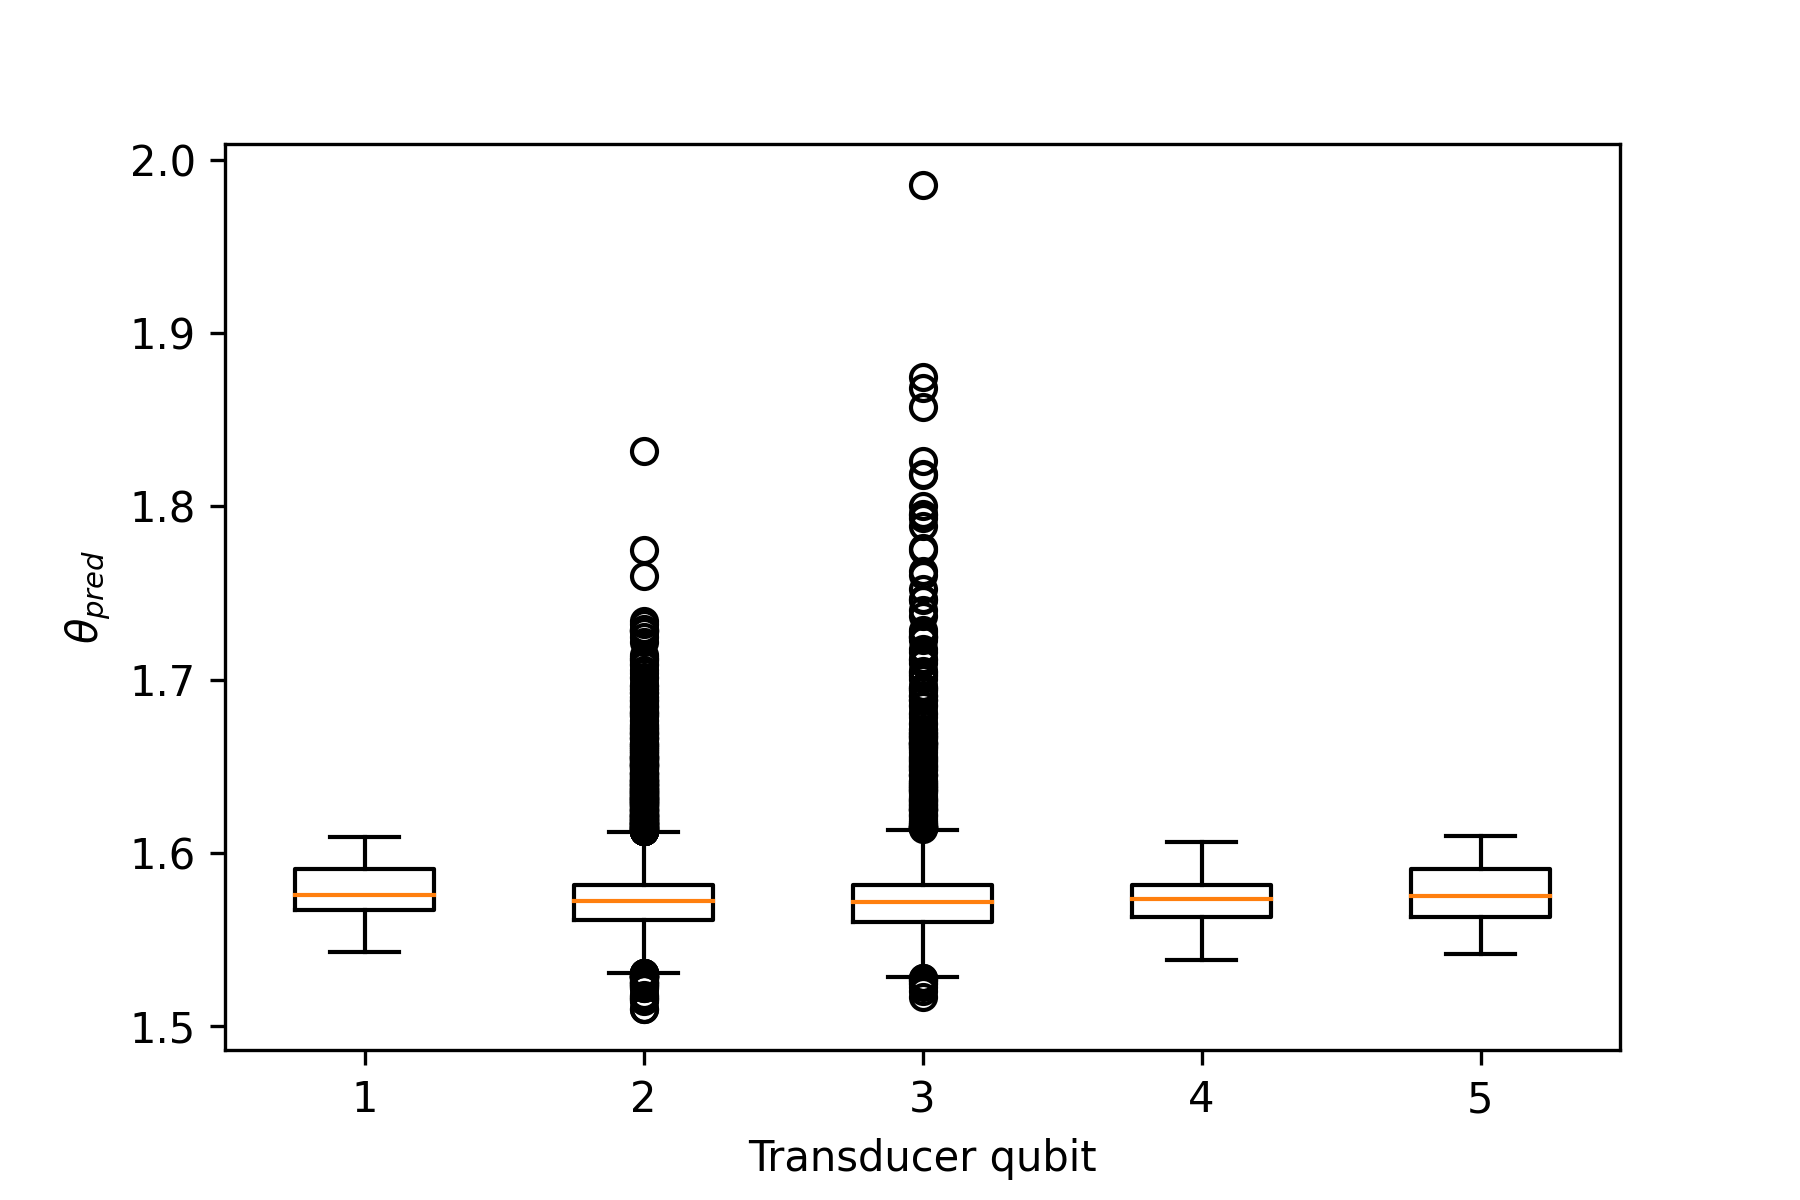
\includegraphics[width=\textwidth]{img/theta_pred_box_dt_1}
	\end{subfigure}
	\begin{subfigure}{0.32\textwidth}
		\centering
		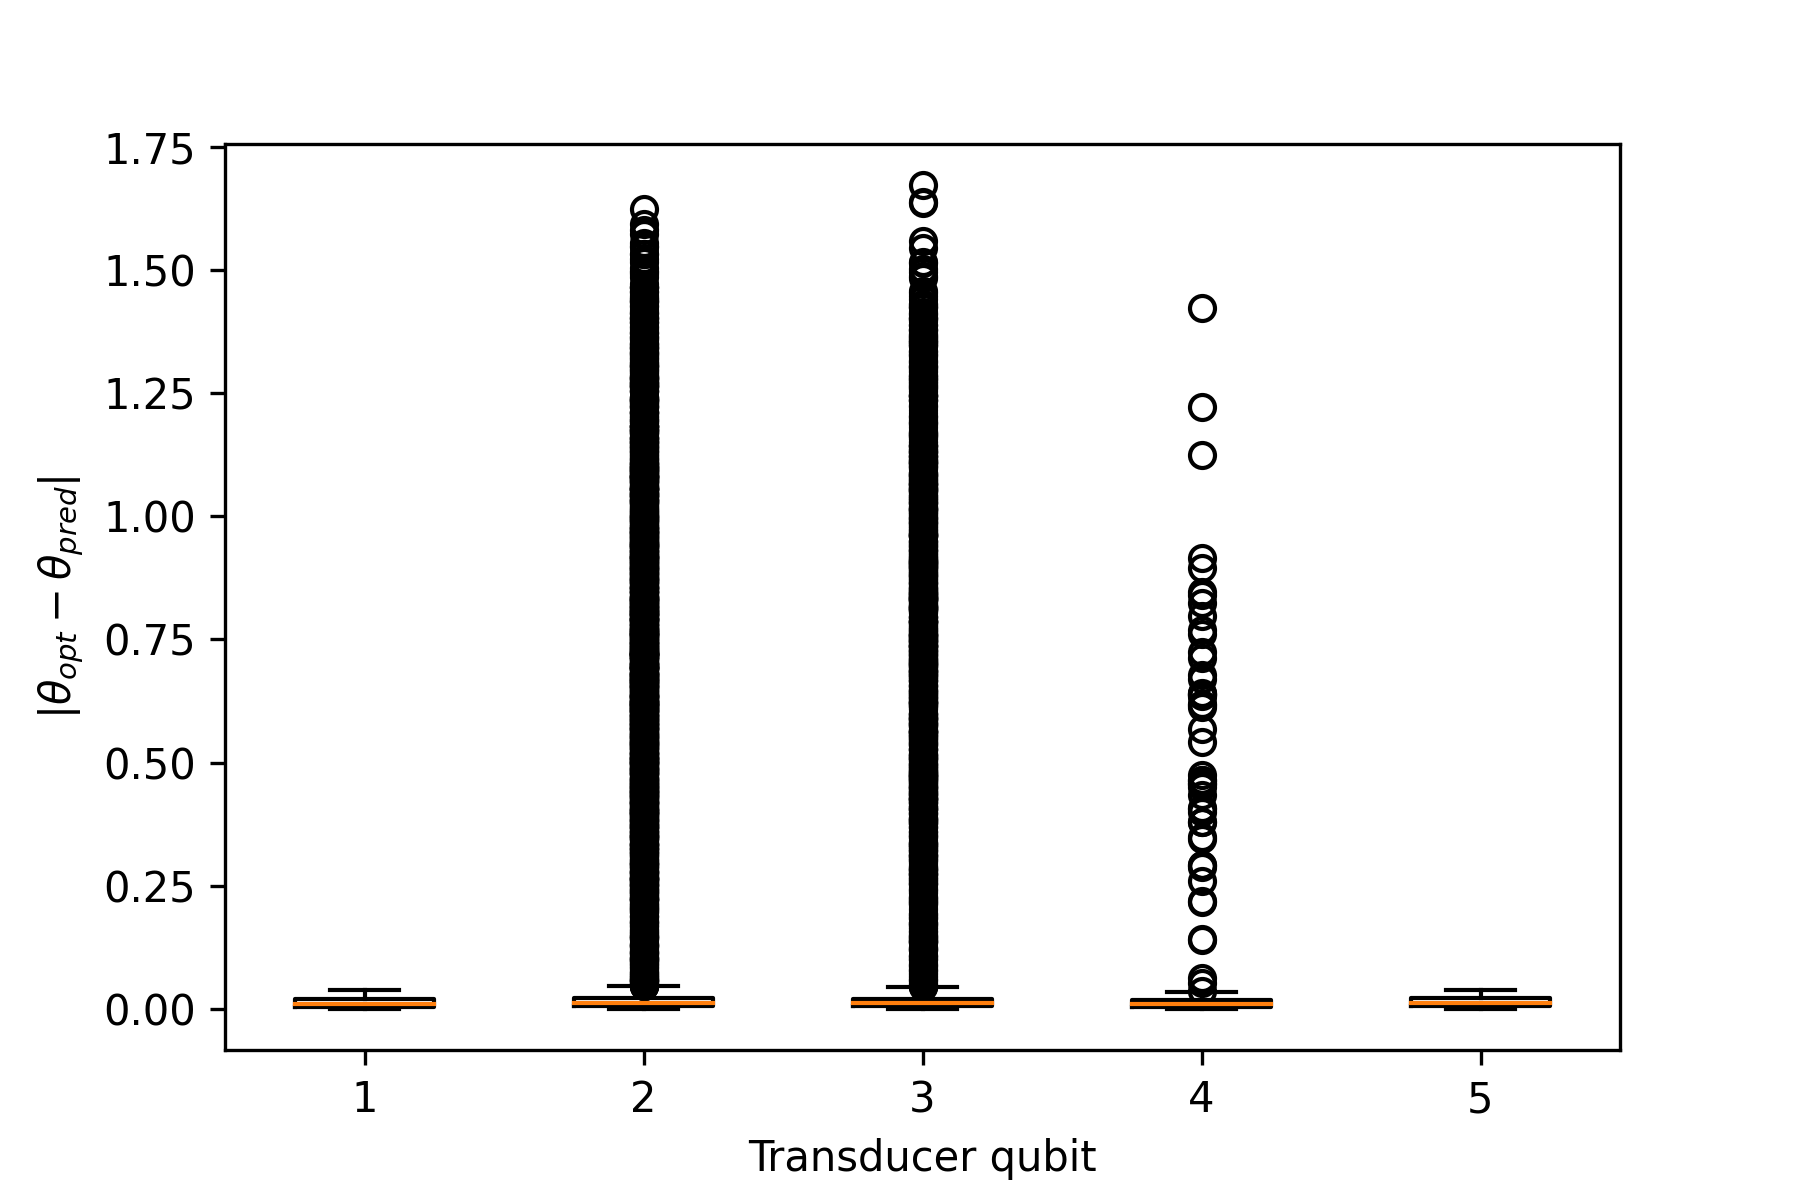
\includegraphics[width=\textwidth]{img/delta_theta_box_dt_1}
	\end{subfigure}
	\begin{subfigure}{0.32\textwidth}
		\centering
		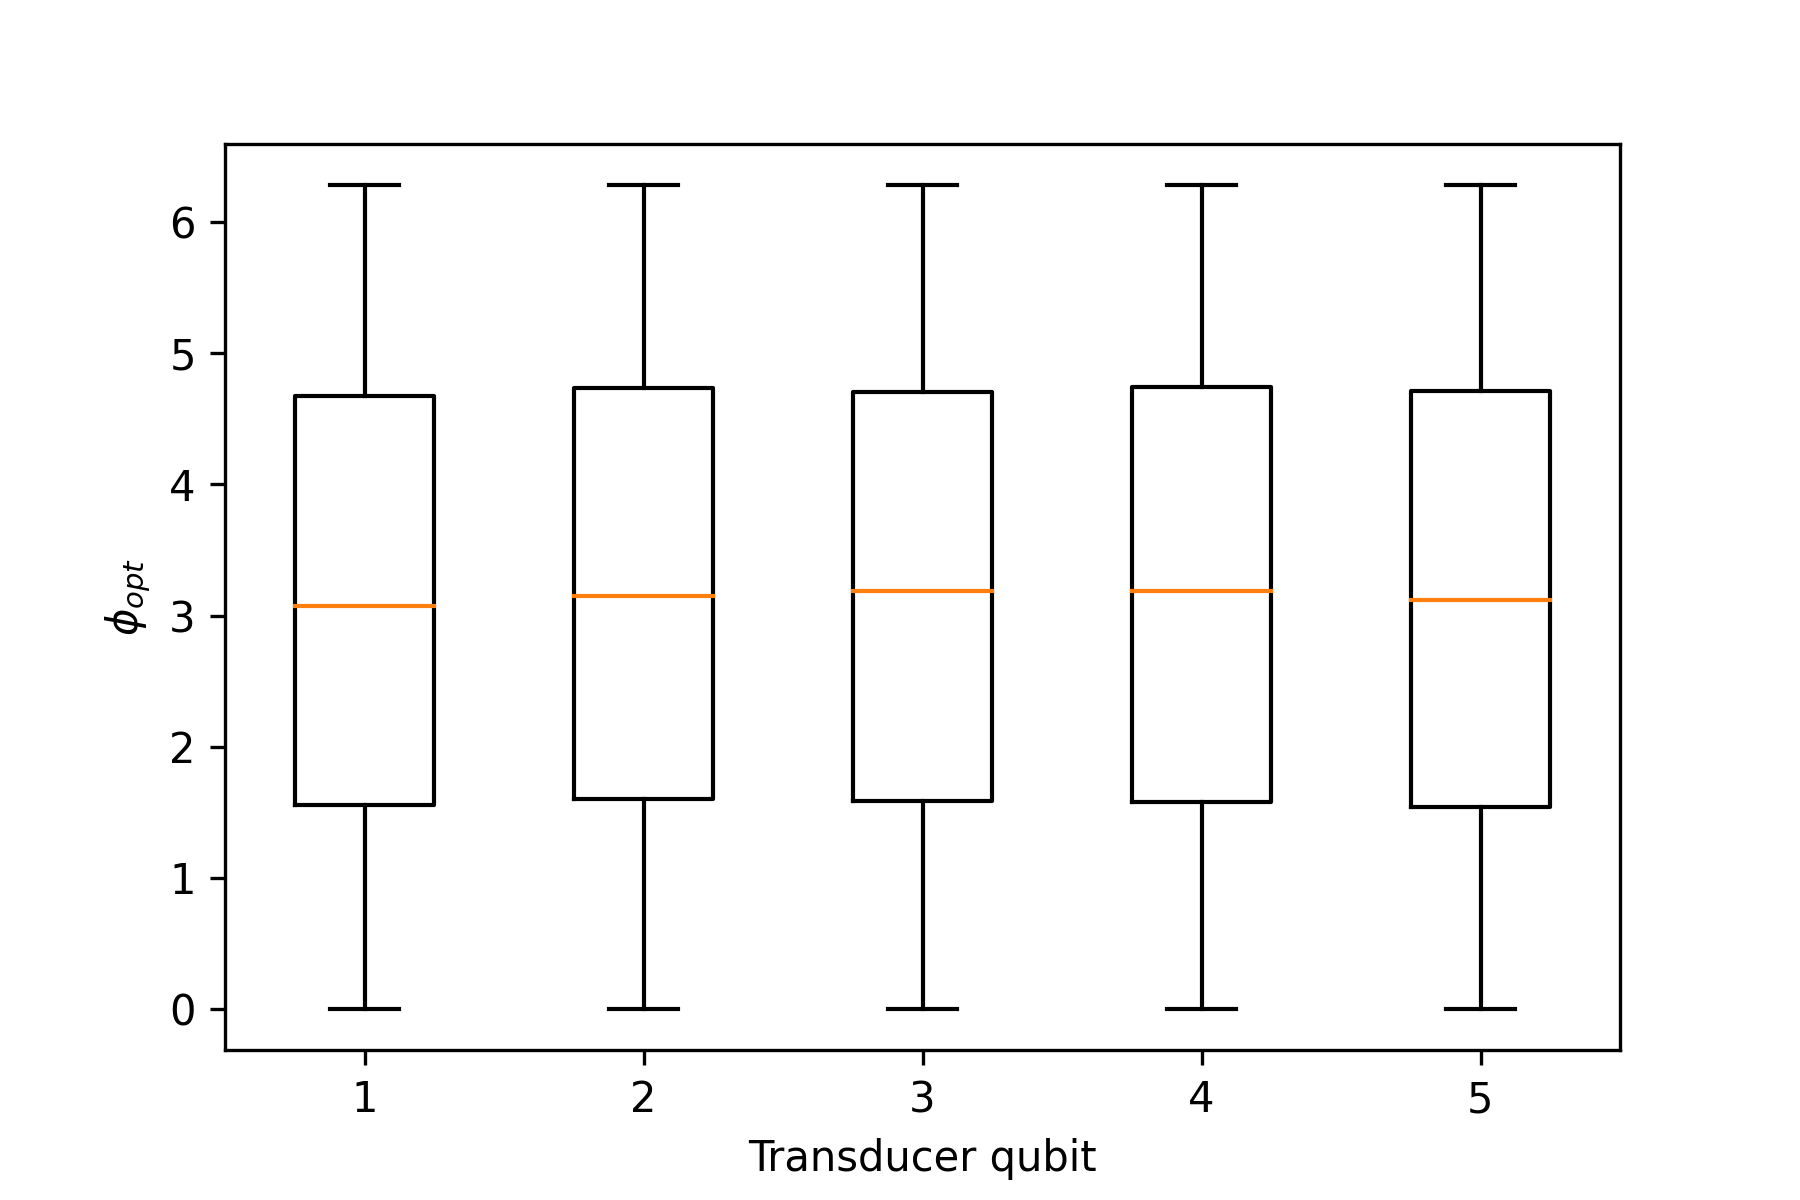
\includegraphics[width=\textwidth]{img/phi_opt_box_dt_1}
	\end{subfigure}
	\begin{subfigure}{0.32\textwidth}
		\centering
		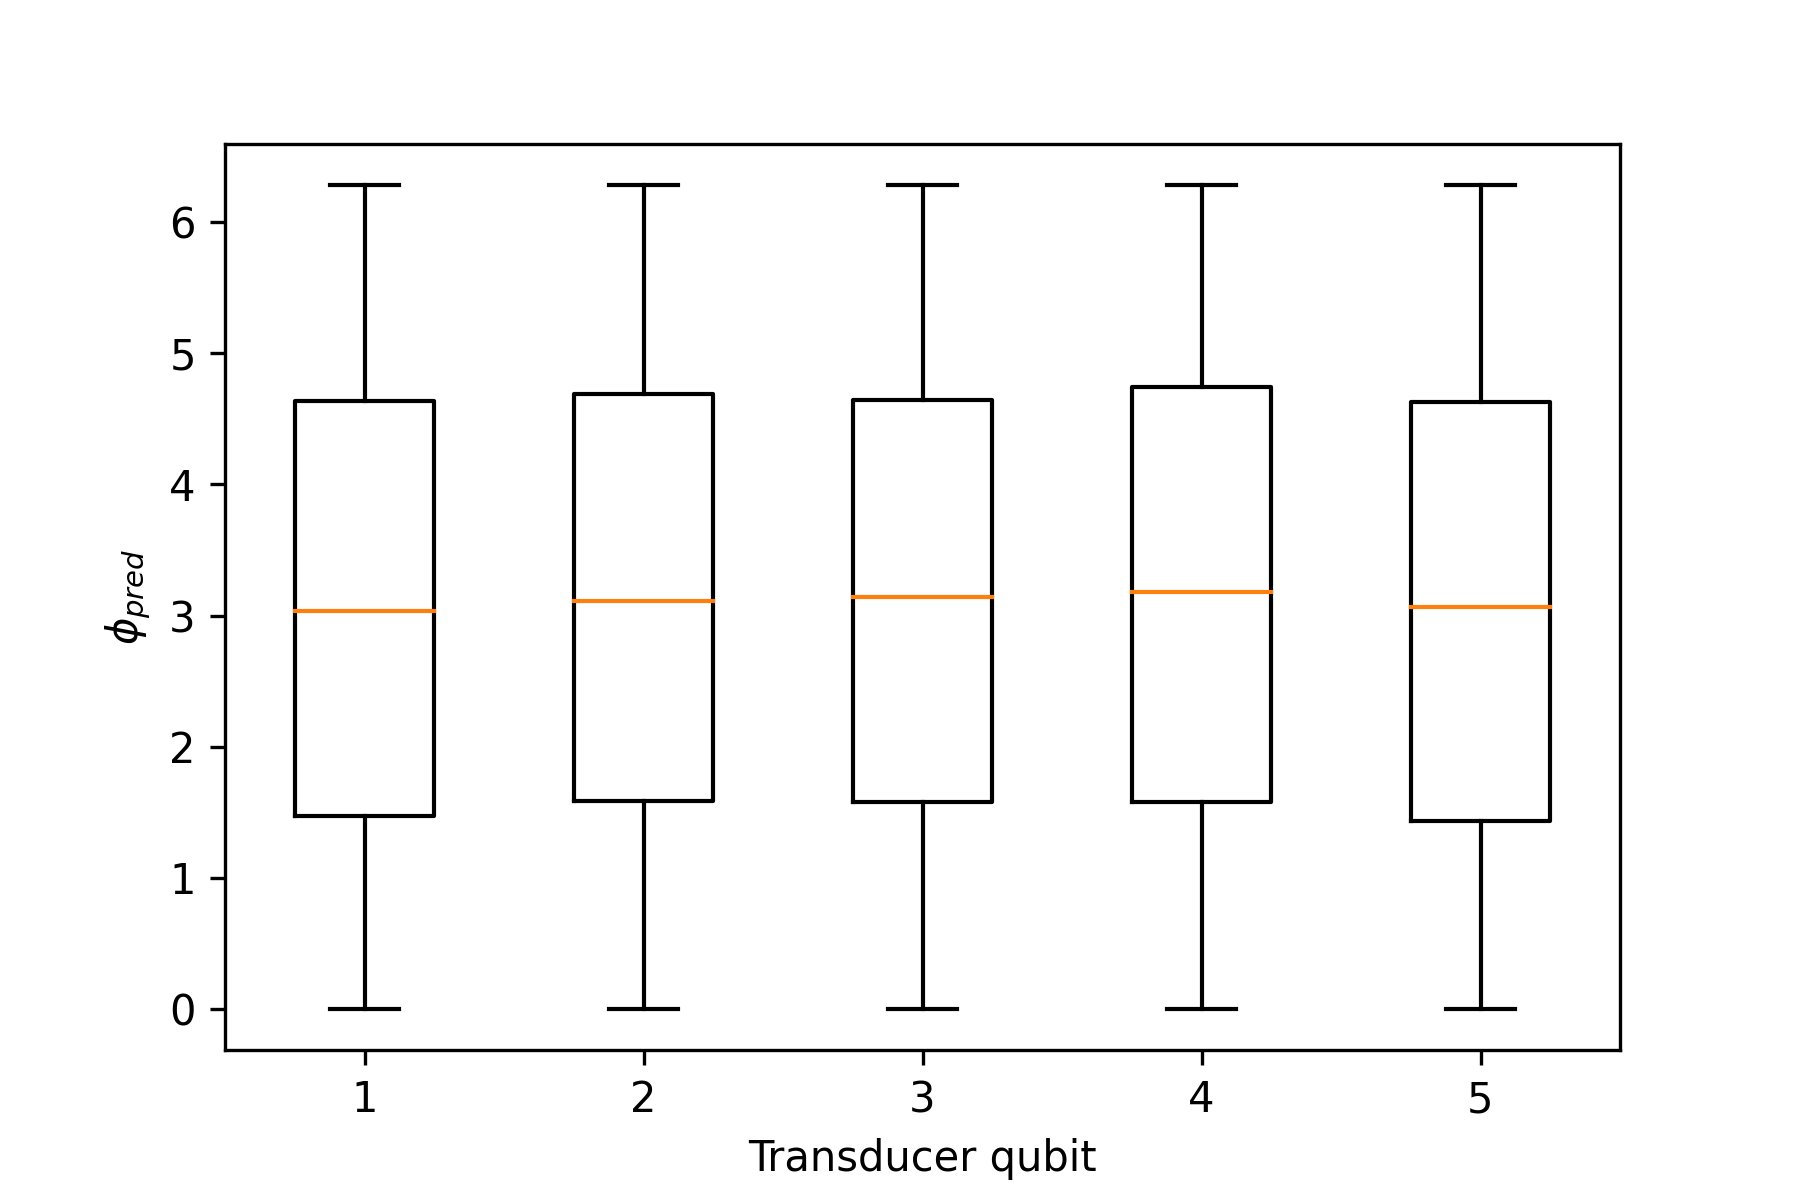
\includegraphics[width=\textwidth]{img/phi_pred_box_dt_1}
	\end{subfigure}
	\begin{subfigure}{0.32\textwidth}
		\centering
		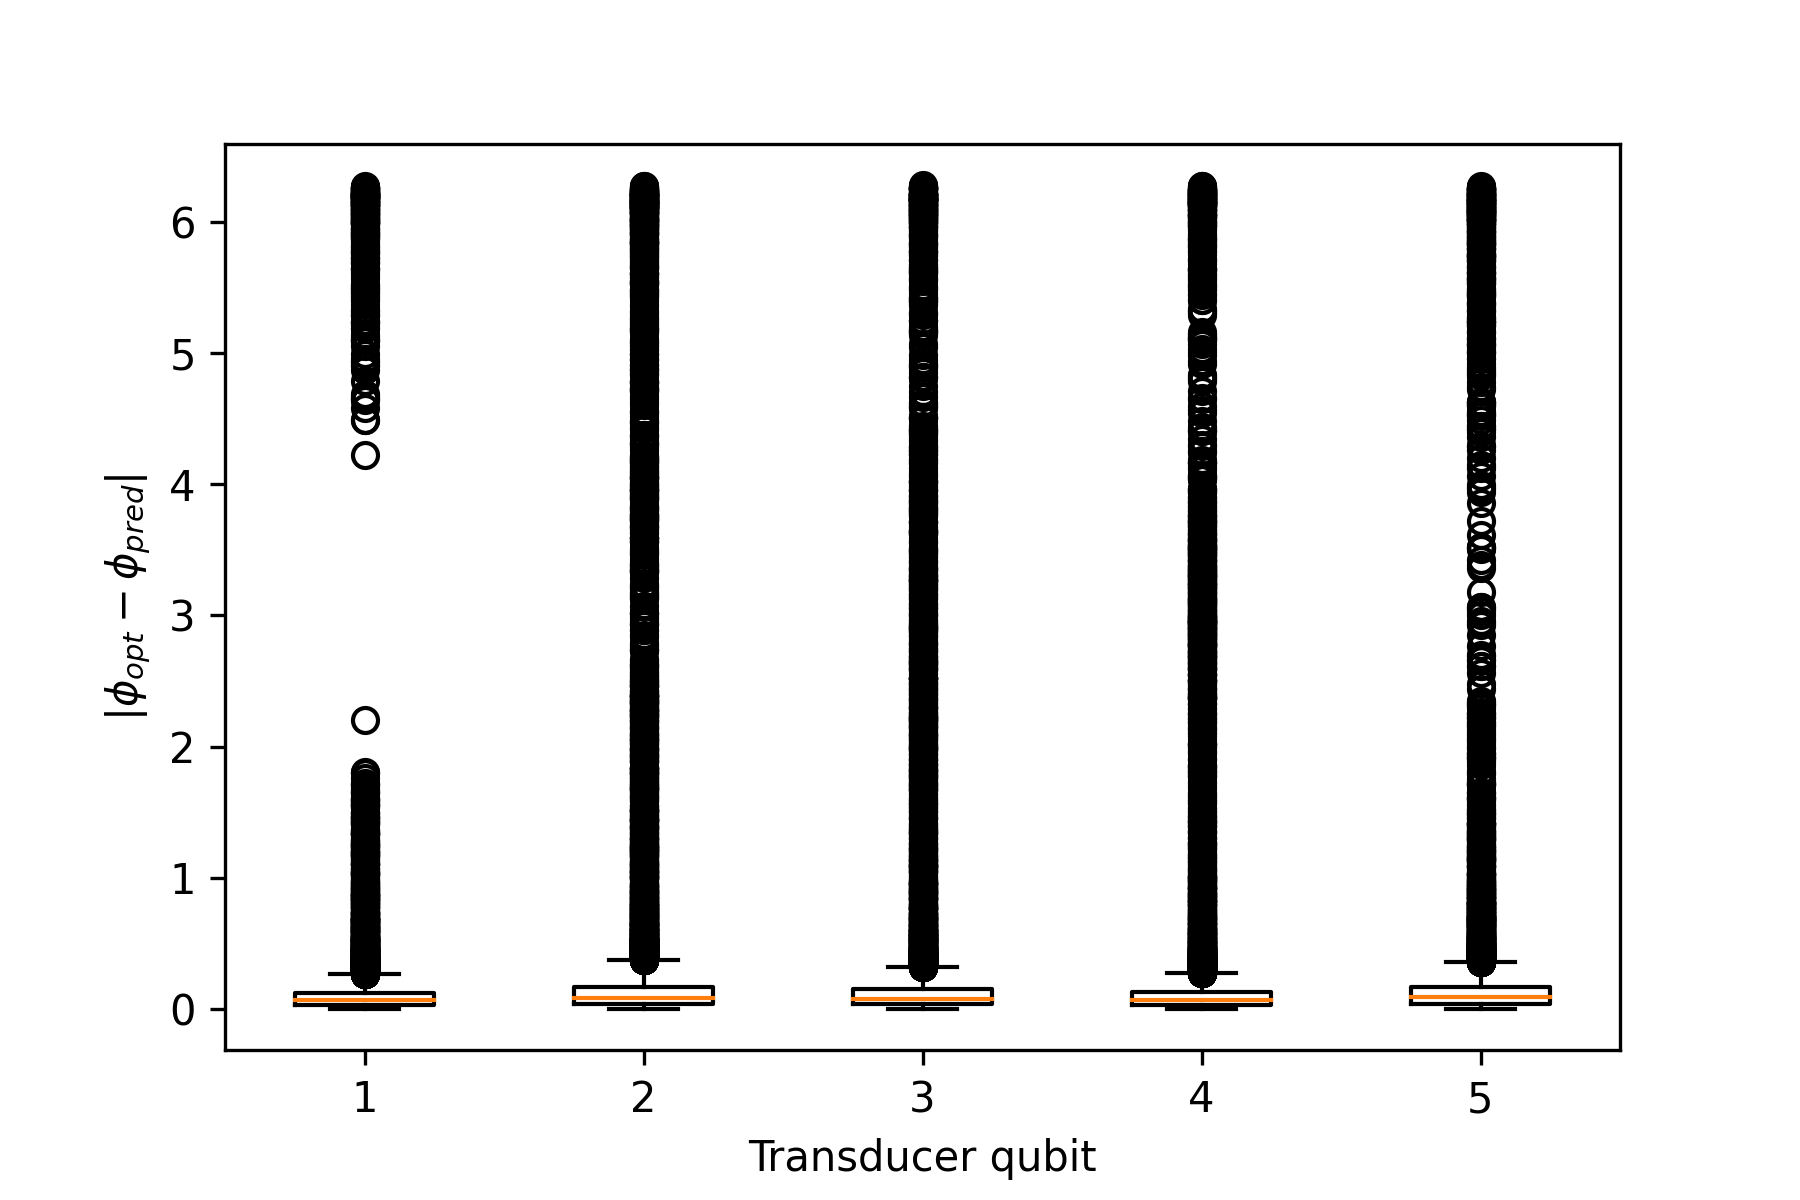
\includegraphics[width=\textwidth]{img/delta_phi_box_dt_1}
	\end{subfigure}
	\caption{\textbf{Top row:} we plot the performance of the bidirectional LSTM on $\theta_T$ for $\Delta \mathrm{T} = 1$. Unlike the optimum for the longer switching time, $\theta_T = \frac{\pi}{2}$ for a majority of the central three qubits as well. For $\Delta \mathrm{T} = 5$, the optimal $\theta_T$ is chosen such that $\Tr{\rho_S \ \sigma_z} = 0$. These states are often unreachable for $\Delta \mathrm{T} = 1$ and the Transducer Hamiltonian strength is maximised instead.  \textbf{Bottom row:} we plot the performance for the Transducer azimuth $\phi_T$.}
	\label{dt1box}
\end{figure}

We illustrate the difference between $\Delta \mathrm{T} = 1$ and $\Delta \mathrm{T} = 5$ in Figure

\begin{table}[h]
	\centering
	\begin{tabular}{ c | c | c | c | c }
		Network Architecture & $\eta_{test} \ [\%]$ & $\mathrm{MSE}_{test}$  & $W_{test}$ & \# Parameters \\
		\hline
		FCANN        & 96.4 & 0.0265 & 1.61 & 8,086,020 \\
		Bidir. LSTM  & 97.4 & 0.0238 & 1.62 & 7,700,222 \\
		Unidir. LSTM & 70.1 & 0.0638 & 1.18 & 3,206,990 \\
		Unidir. LSTM, higher cell state dimension & 69.9 & 0.0637 & 1.17 & 7,704,062 \\
	\end{tabular}
	\caption{Efficiencies $\eta$ and MSE loss on the test set for differing model architectures for $N=5, \Delta \mathrm{T} = 1$.}
	\label{effdt1}
\end{table}


\begin{figure}
	\centering
	\begin{subfigure}{0.85\textwidth}
		\centering
		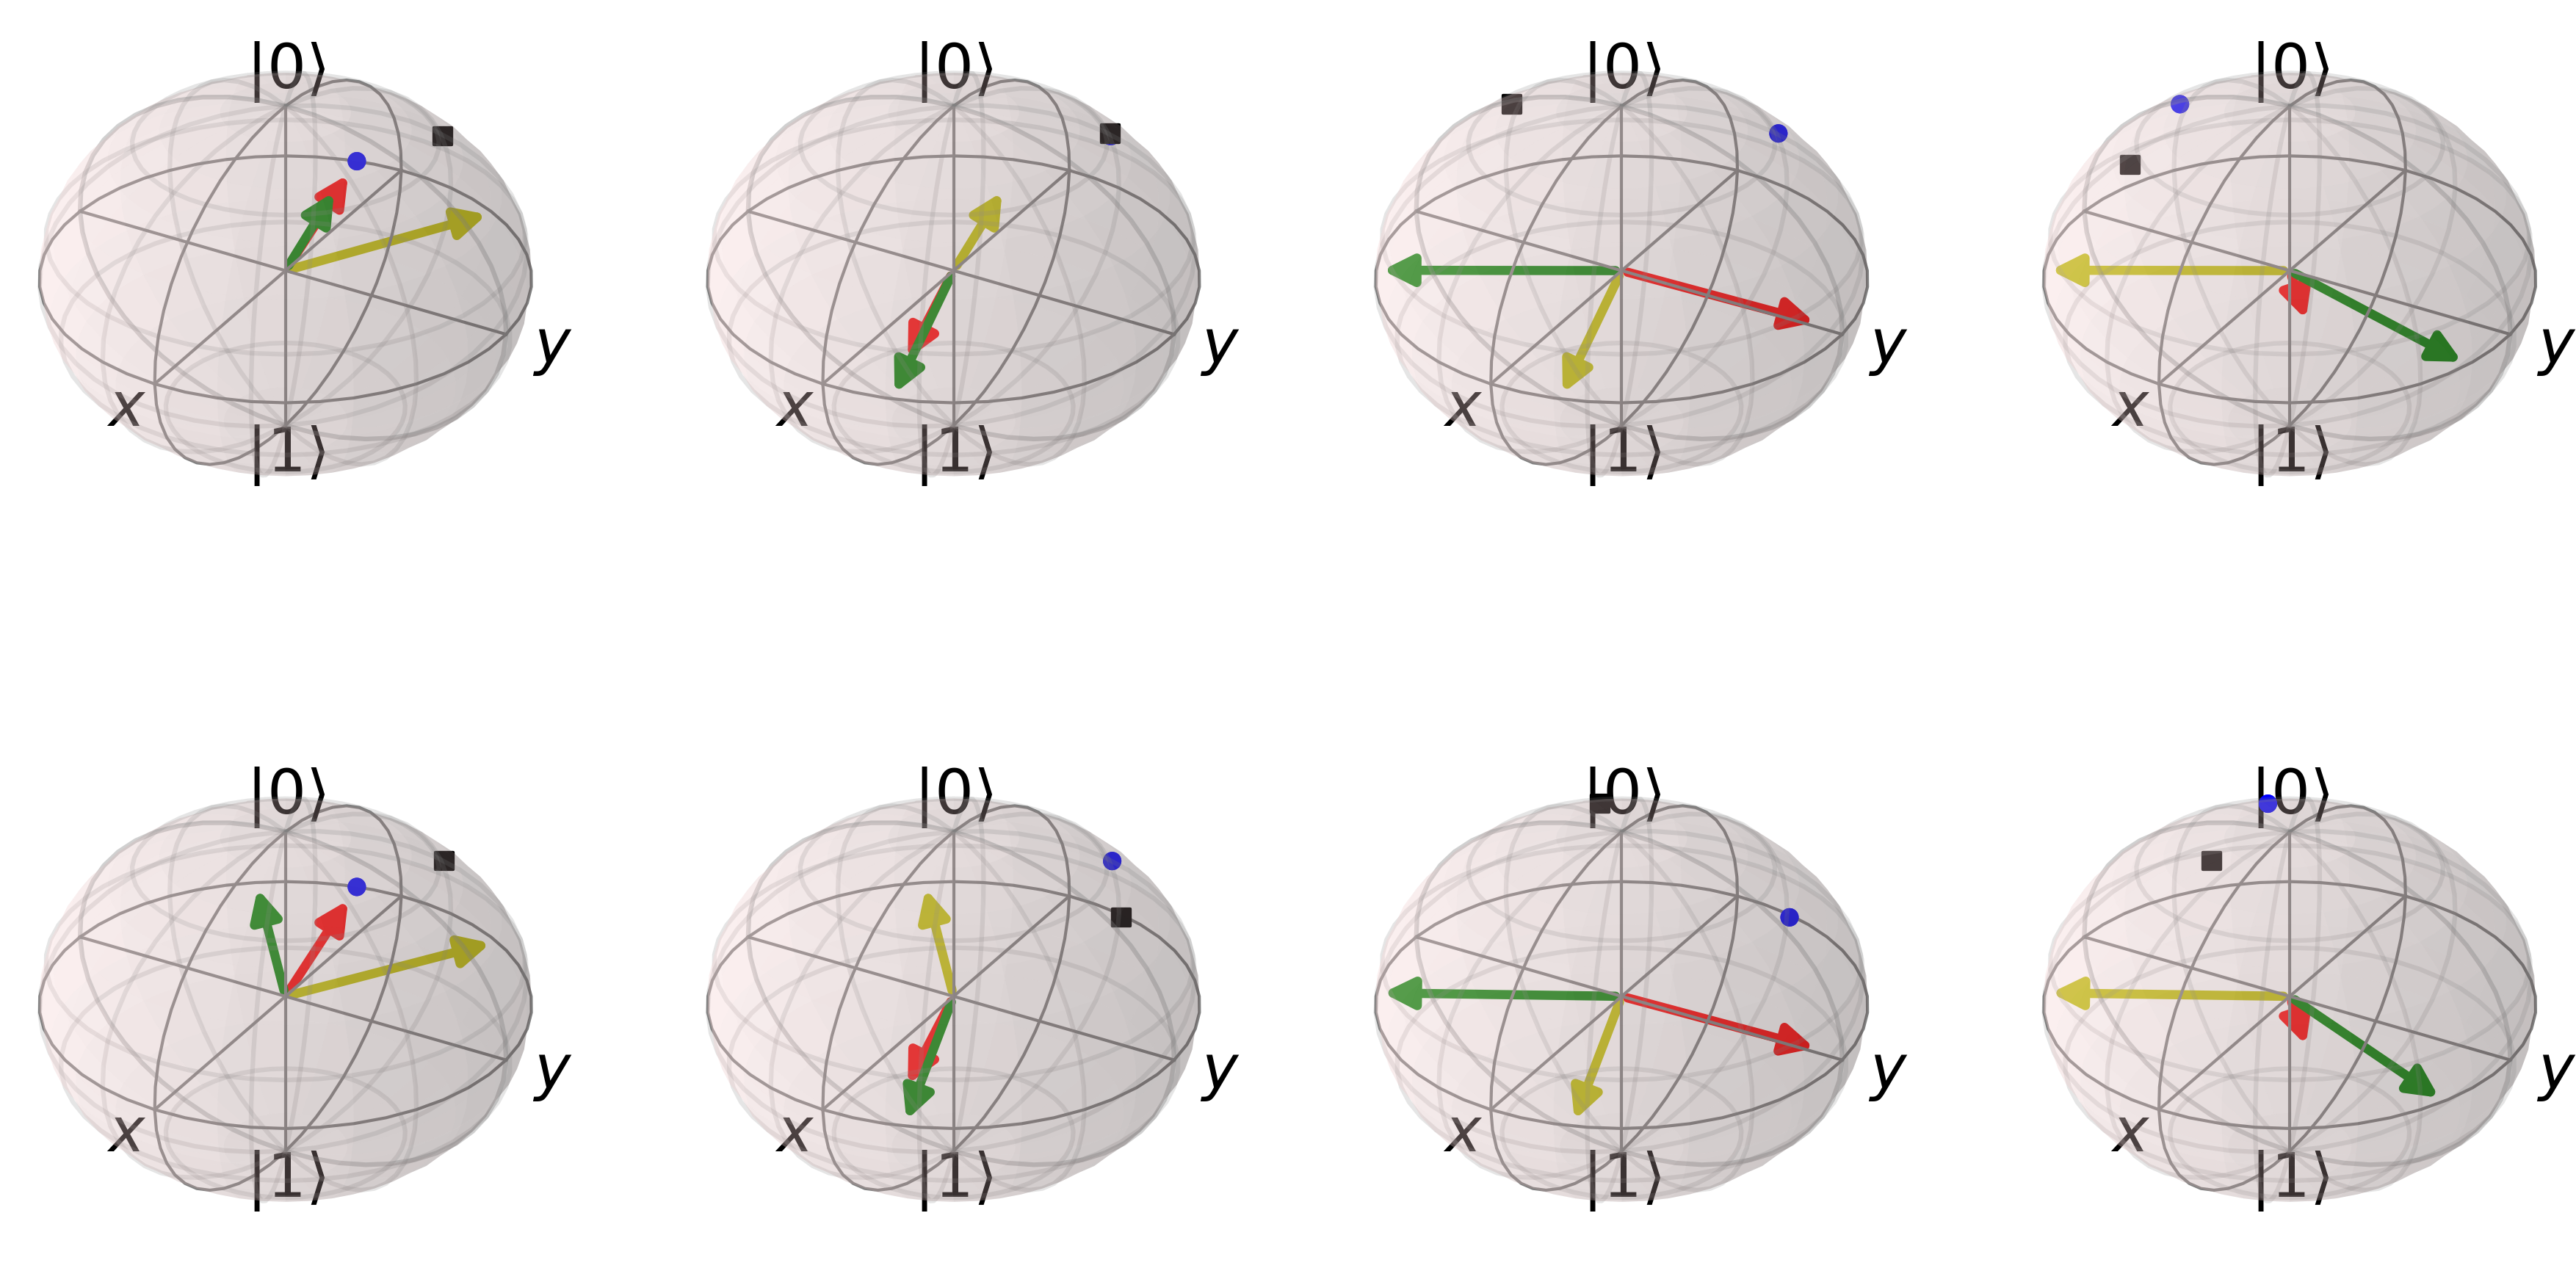
\includegraphics[width=\textwidth]{img/bloch_comp_1_crop}
		\caption{$\Delta \mathrm{T} = 1: W_{opt} = 1.40, W_{pred} = 1.32$}
		\label{}
	\end{subfigure}
	\begin{subfigure}{0.85\textwidth}
		\centering
		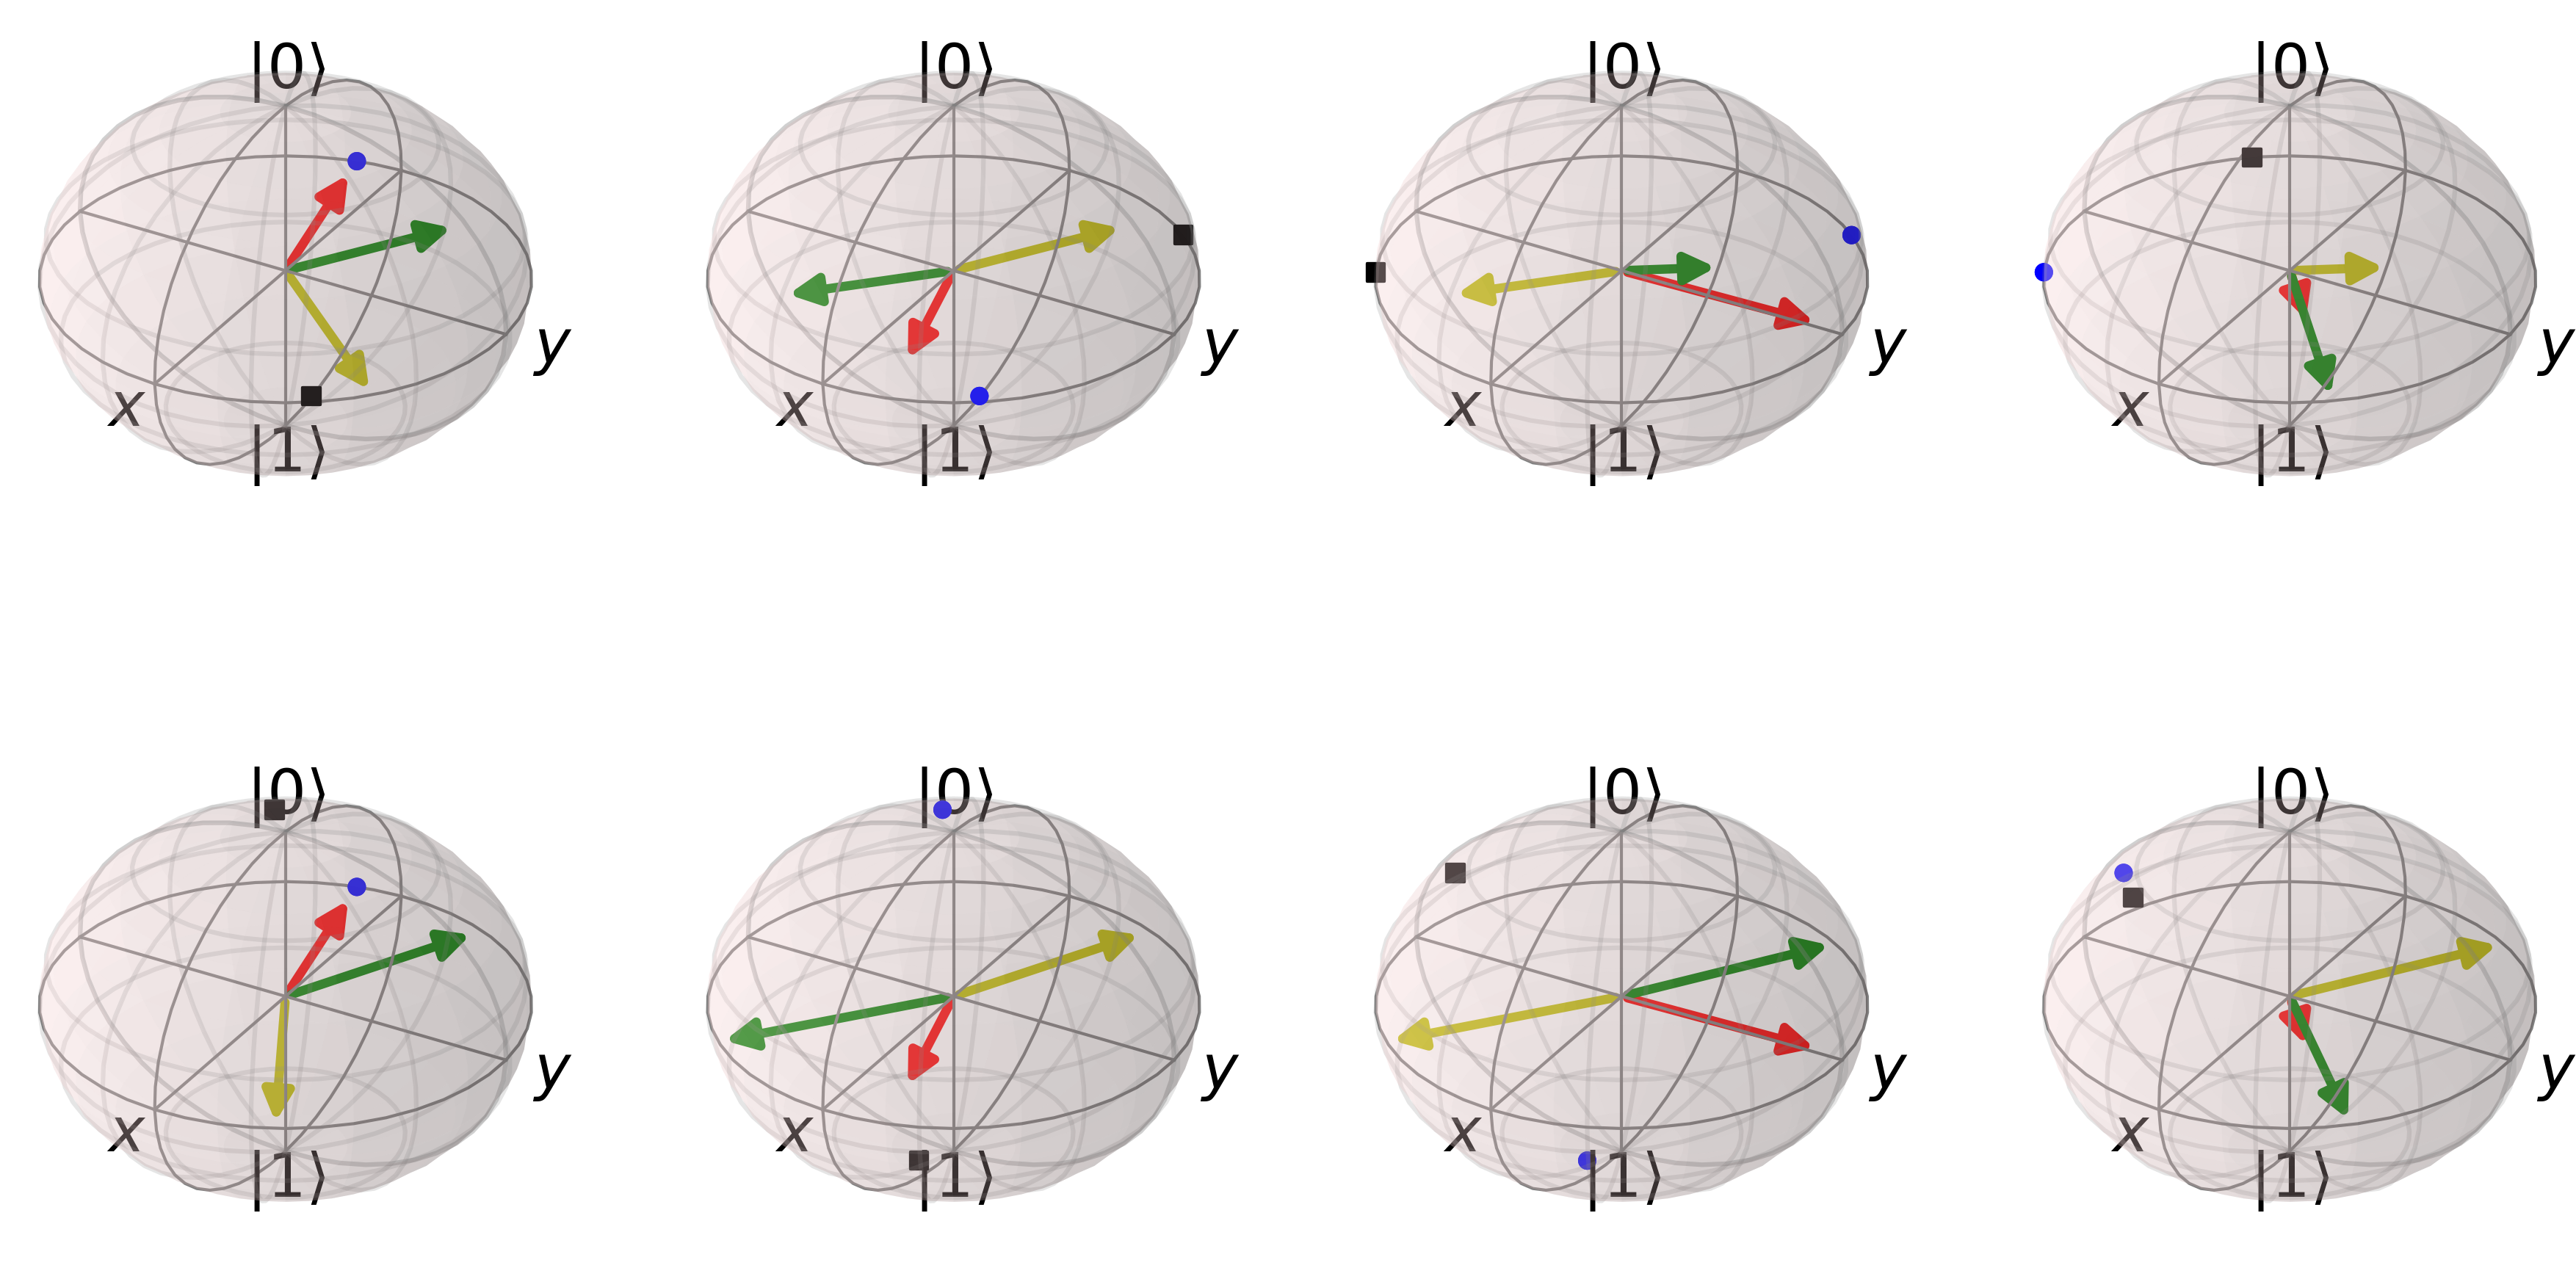
\includegraphics[width=\textwidth]{img/bloch_comp_5_crop}
		\caption{$\Delta \mathrm{T} = 5: W_{opt} = 2.42, W_{pred} = 0.57$}
		\label{}
	\end{subfigure}
	\caption{We plot the optimal (top row) and predicted (bottom row) system state and Transducer settings for the bidirectional LSTM, using the same representations as in Figure \ref{n_5_blochs}, for $\Delta \mathrm{T} = 1$ (a) and $\Delta \mathrm{T} = 5$ (b). The Drive sequence is the same in all rows and is a sample from the test set. For $\Delta \mathrm{T} = 1$, the optimal system state, where $\Tr{\rho_S^i \sigma_z} = 0$, cannot be reached.}
	\label{}
\end{figure}

\subsection{Noise resistance}\label{ml_noise}
% !TeX spellcheck = en_GB
Besides the efficiency of the networks the resistance of their predictions to noise is also of interest.
We create a noisy sequence $\{\ket{\phi_j}\}$ of N qubits from $\{\ket{\psi_j}\}$ using
\begin{align*}
	\ket{\phi_j} = e^{-i H_j \tau} \ket{\psi_j} \ \forall j \in [1, N].
\end{align*}
$H_j$ are randomly generated Hermitian matrices with $\norm{H_j} = 1$ and $\tau$ is a real parameter used to control the strength of the noise.
To quantify the dissimilarity between $\{\ket{\phi_j}\}$ and $\{\ket{\psi_j}\}$ we use the fidelity $F$ as defined in \cite{10.5555/1972505}:
\begin{align*}
	F_{\text{run}}(\{\ket{\phi_j}\}, \{\ket{\psi_j}\}) = \prod_j F(\ket{\phi_j}, \ket{\psi_j}) = \prod_j \abs{\bra{\phi_j}\ket{\psi_j}}.
\end{align*}

The performance of the bidirectional LSTM for $\Delta \mathrm{T} = 1$ and $\Delta \mathrm{T} = 5$ on noisy sequences is presented in Figure \ref{noisedt5}.
For $\Delta \mathrm{T} = 1$, the performance degrades among the test set, as the noiseless predictions are near their optima.
The variance in the deviation of work output between noisy and noiseless data $\Delta W$ is larger for $\Delta \mathrm{T} = 5$ as the longer evolution time leads to a larger difference between the system states of the noisy and noiseless case.
As the network is less likely to predict a solution near the optimum, the noisy data will sometimes be closer to the optimum and thus a significant amount of data points with $\Delta W > 0$ exist as well.

\begin{figure}[h]
	\centering
	\begin{subfigure}{0.4\textwidth}
		\centering
		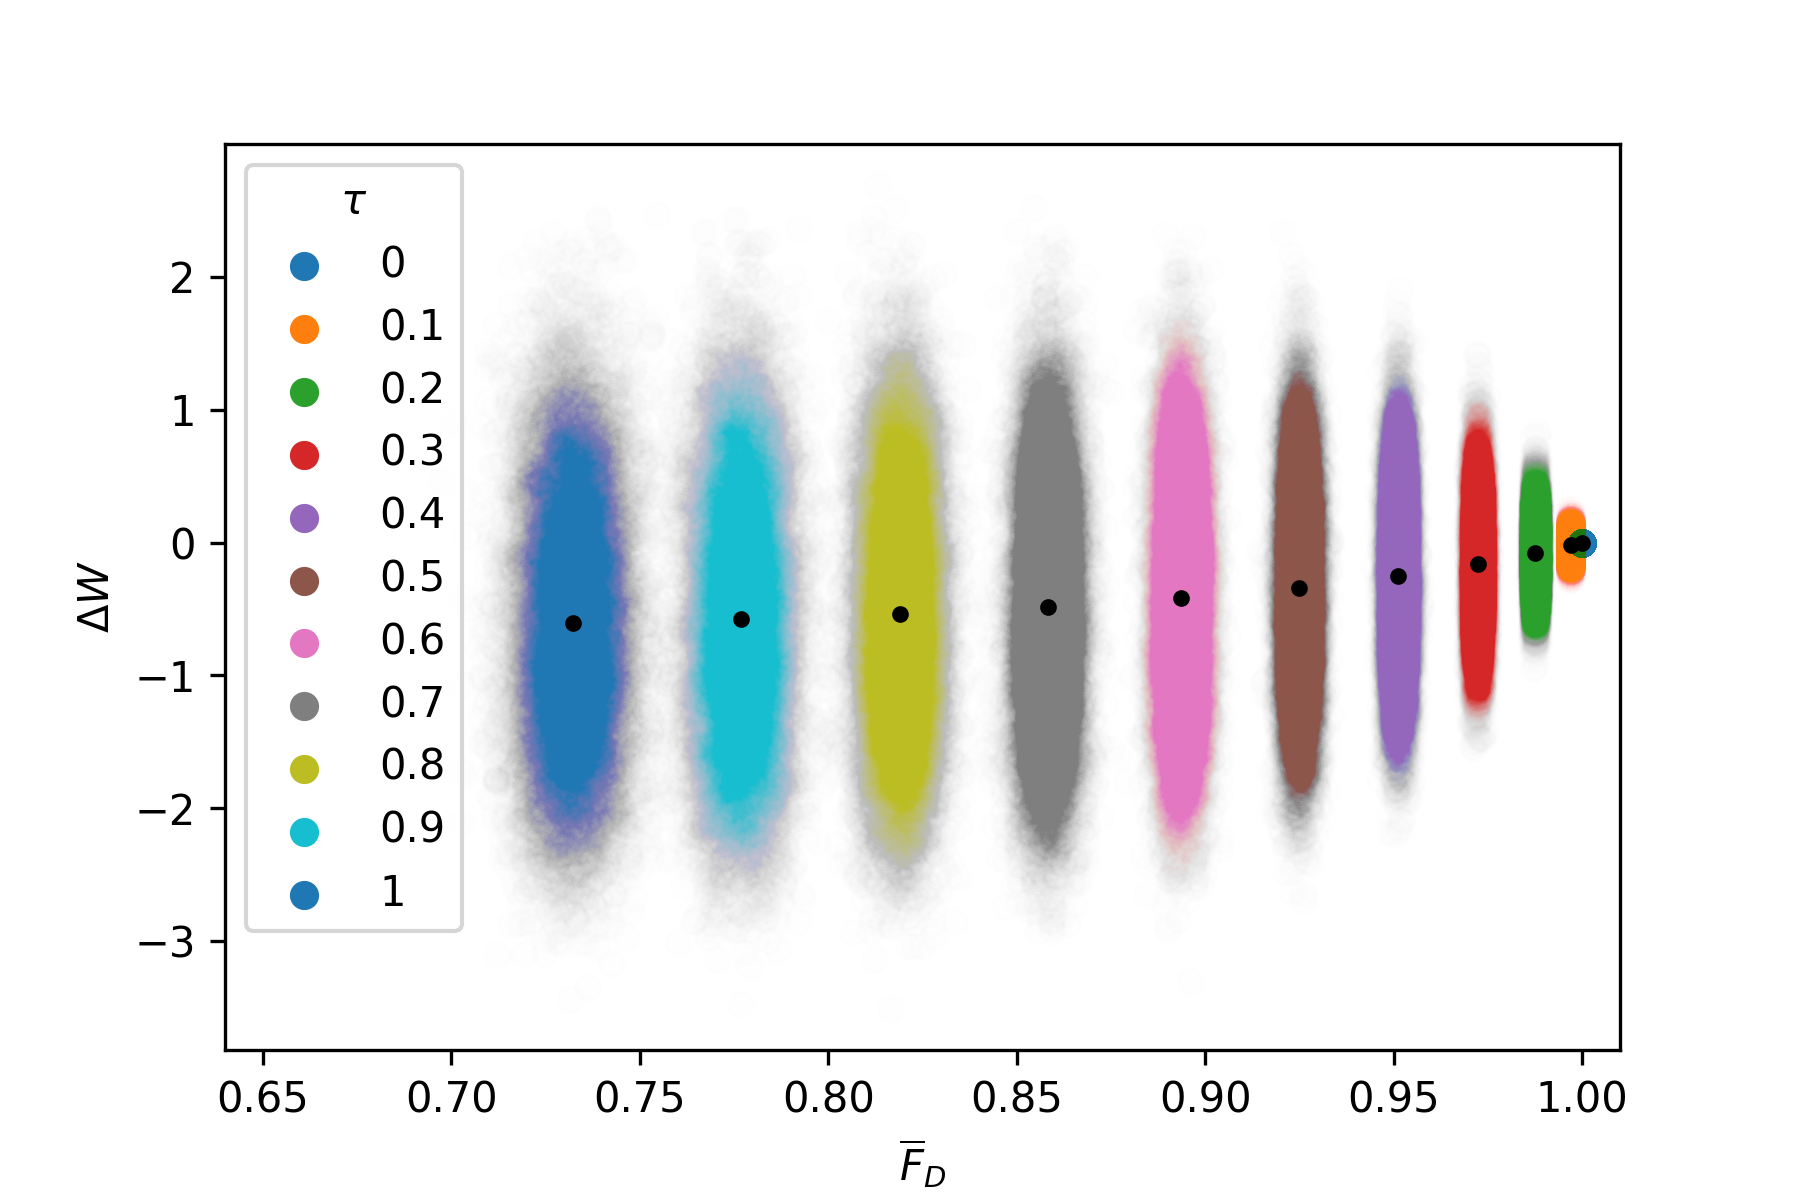
\includegraphics[width=\textwidth]{img/noisy_drive_bi_true_3}
		\subcaption{Noisy drive sequence, $\Delta \mathrm{T} = 5$}
	\end{subfigure}
	\begin{subfigure}{0.4\textwidth}
	\centering
	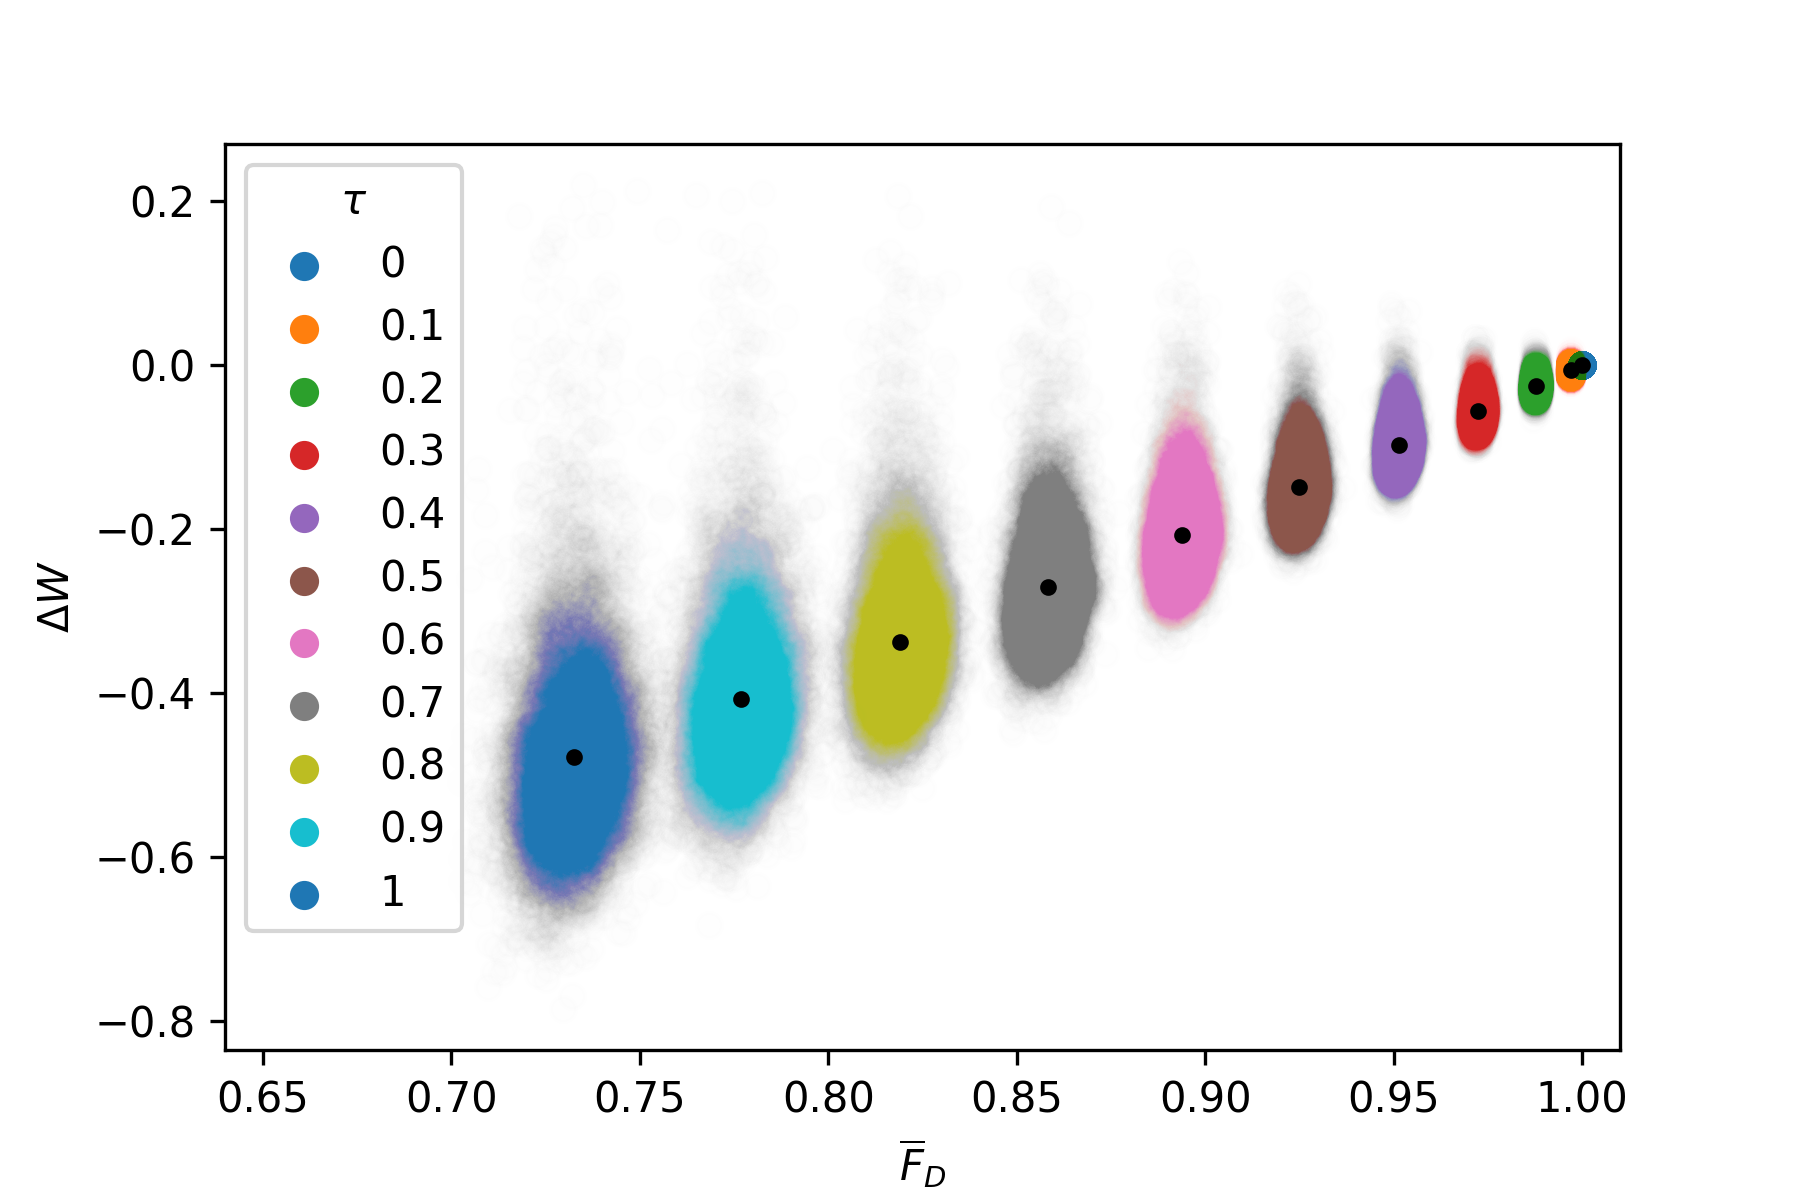
\includegraphics[width=\textwidth]{img/noisy_drive_dt_1}
	\subcaption{Noisy drive sequence, $\Delta \mathrm{T} = 1$}
	\end{subfigure}
	\begin{subfigure}{0.4\textwidth}
		\centering
		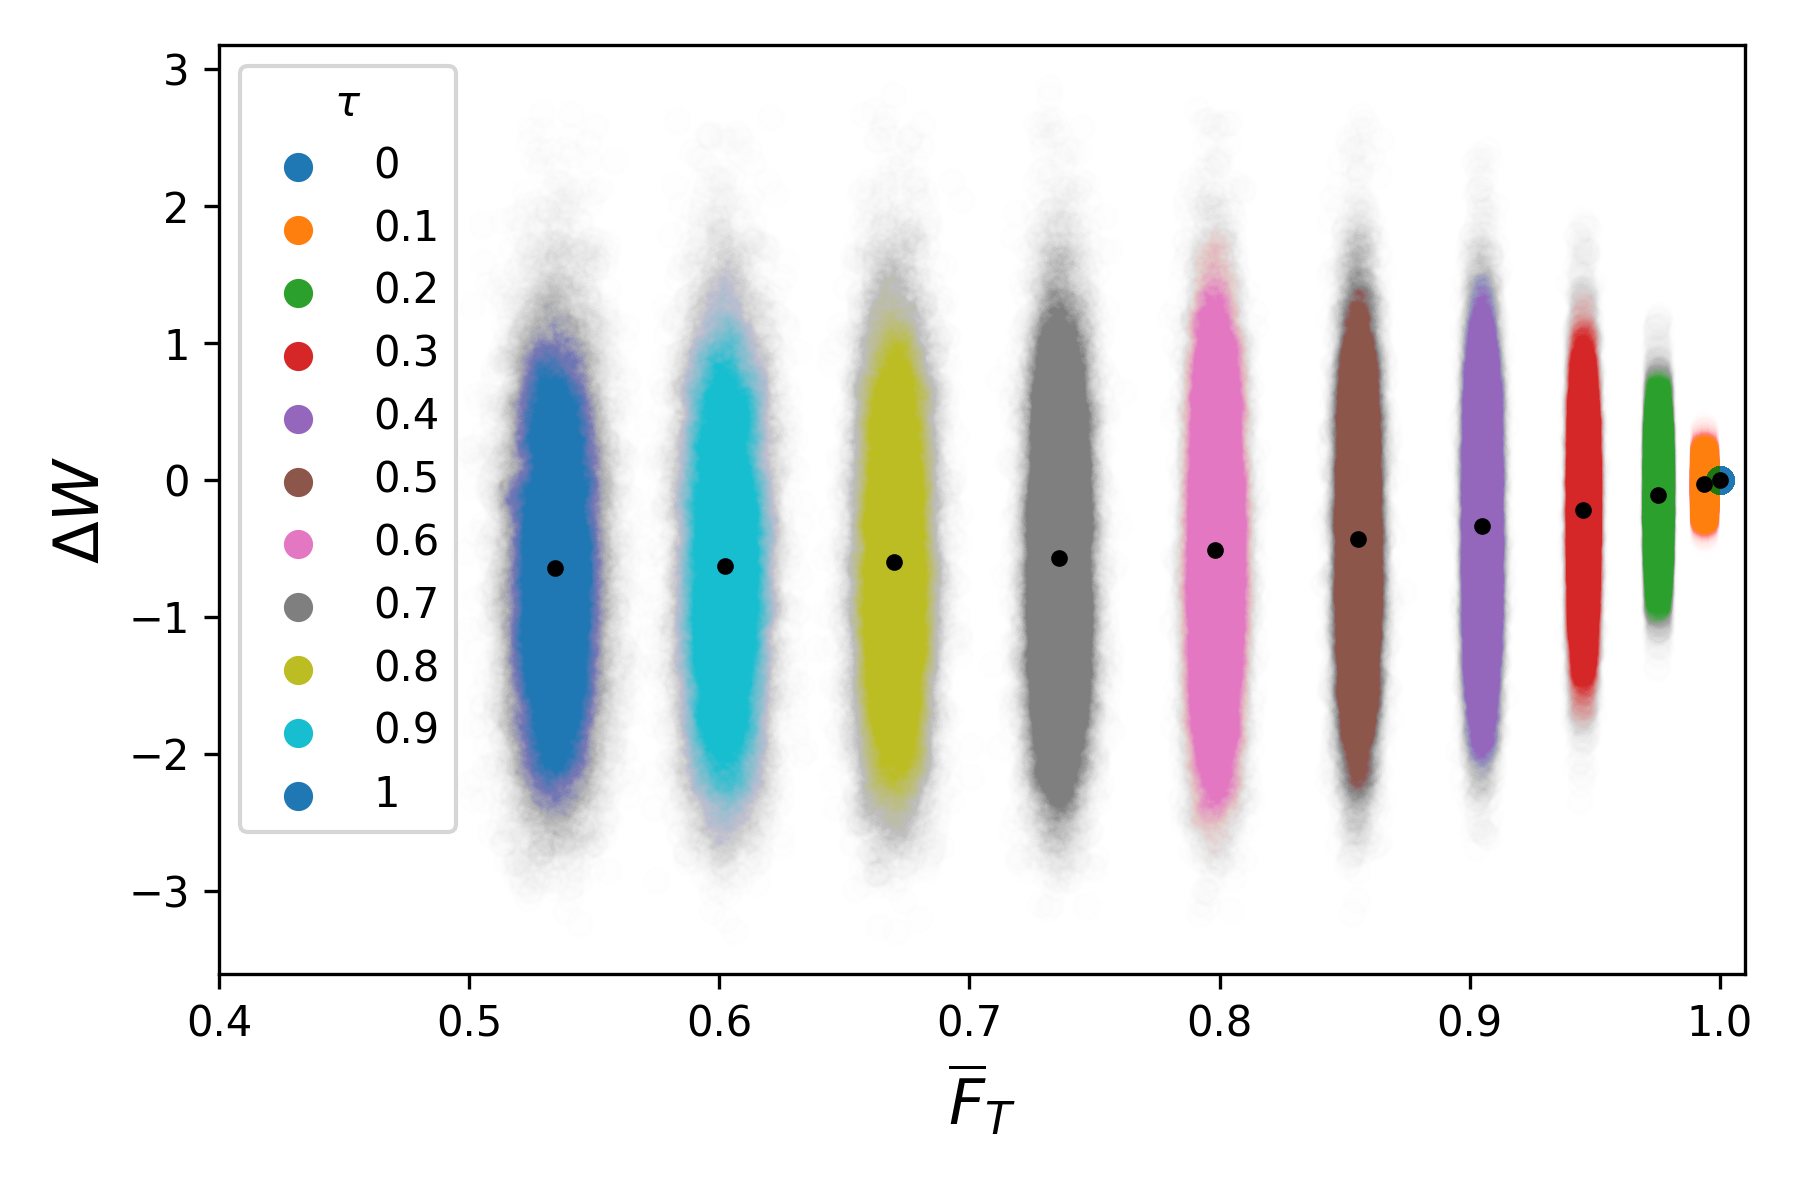
\includegraphics[width=\textwidth]{img/noisy_trans_bi_true_3}
		\subcaption{Noisy transducer sequence, $\Delta \mathrm{T} = 5$}
	\end{subfigure}
	\begin{subfigure}{0.4\textwidth}
		\centering
		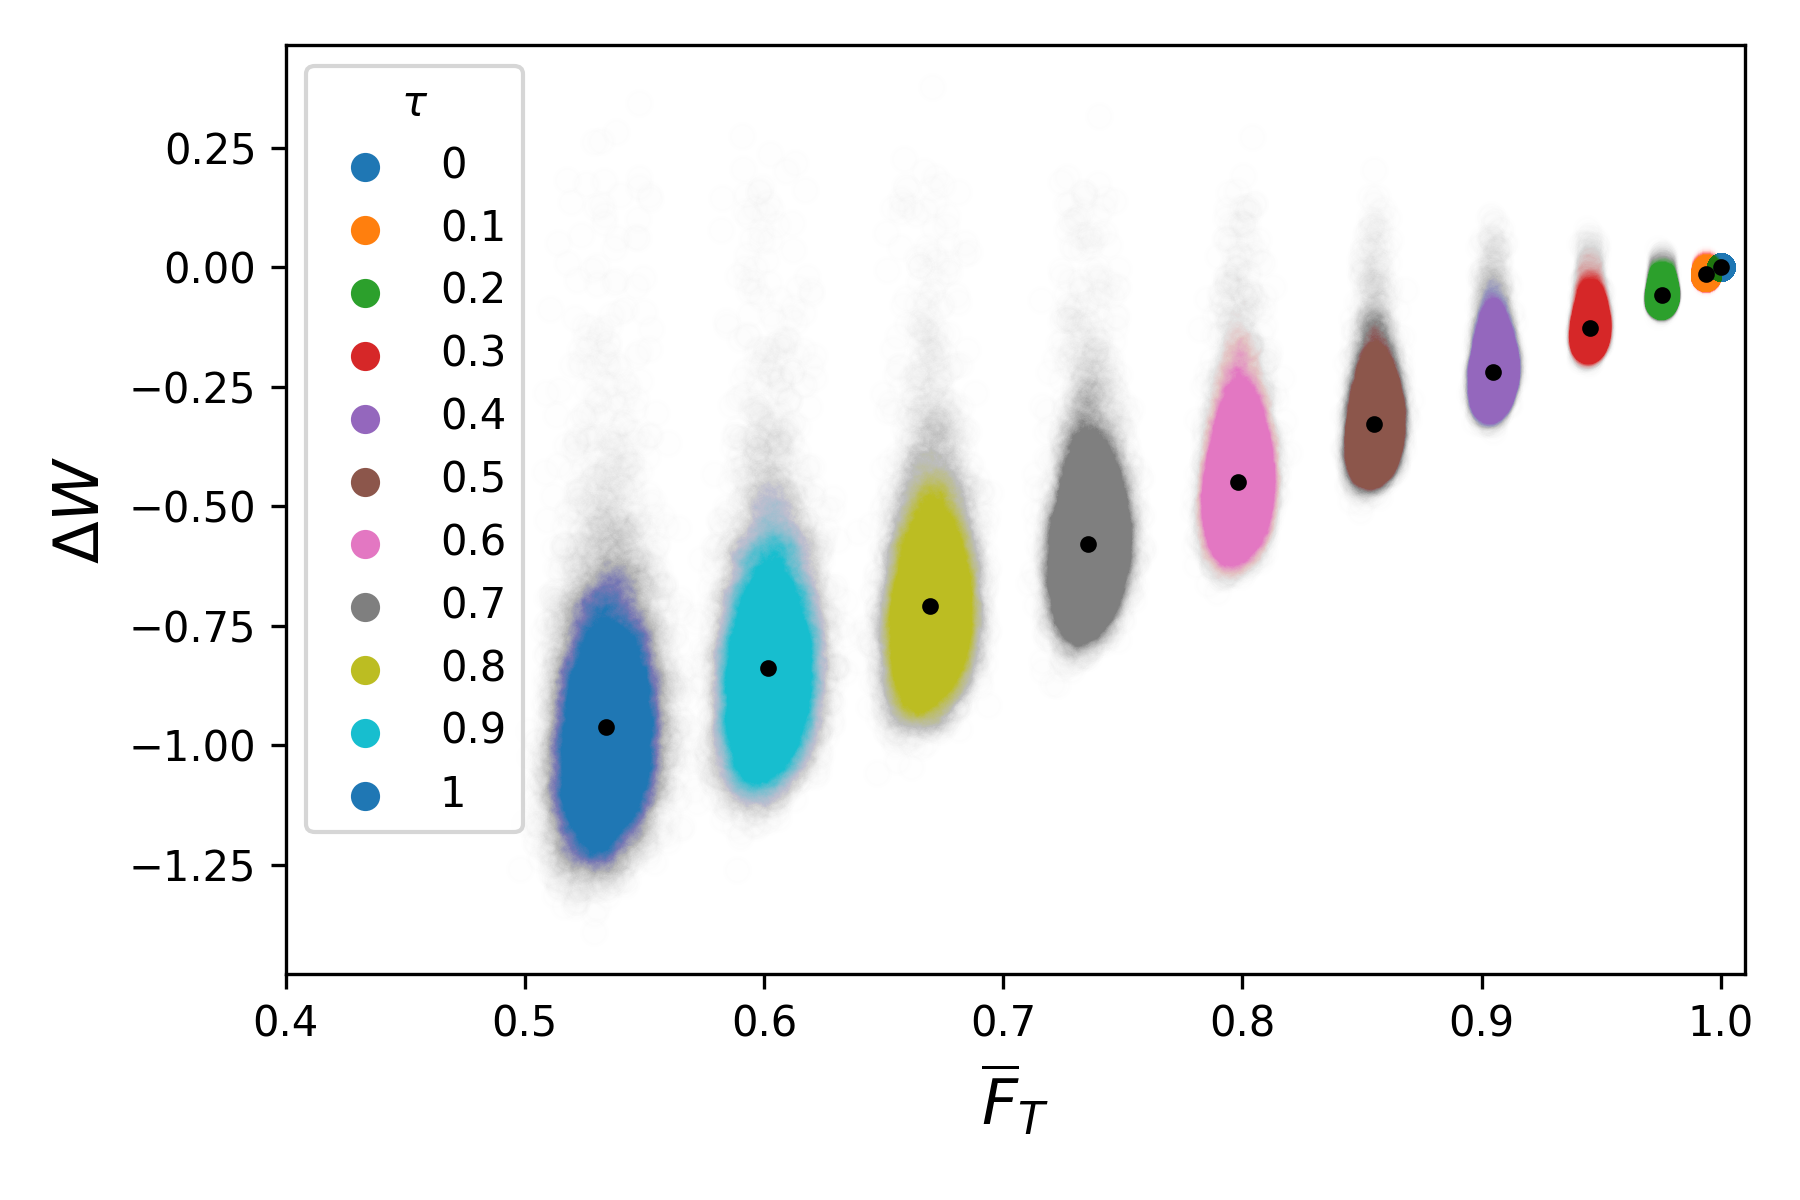
\includegraphics[width=\textwidth]{img/noisy_trans_dt_1}
		\subcaption{Noisy transducer sequence, $\Delta \mathrm{T} = 1$}
	\end{subfigure}
	\caption{We plot the difference $\Delta W = \overline{W}_{noise} - W_{pred}$ of each element of the test set for the bidirectional LSTM. $W_{pred}$ is the work output following the model prediction. \textbf{(a), (b)} We create 100 noisy drive sequences and calculate the average $\overline{W}_{noise}$ of their work output following the predicted transducer protocol. \textbf{(c), (d)} We create 100 noisy transducer sequences and calculate the average of their work output with a given drive sequence from the test set. In both plots, the black dots indicate the average fidelities and $\Delta W$ for a given $\tau$.}
	\label{noisedt5}
\end{figure}

\subsection{Extracted work as cost function}\label{work_cost}
% !TeX root = ../BA_main_englisch.tex
% !TeX spellcheck = en_GB
In Section \ref{n_5_ml} we encountered a conceptional problem regarding using the MSE as a loss function, where a low MSE score does not necessarily imply a large work output.
In the following we aim to investigate whether directly using extracted work $W$ as the network cost function can improve performance.

%To ensure comparability between the different cost functions, we continue using the same hyperparameters to train both a bidirectional and a unidirectional LSTM.
%The performance for both networks and two switching times $\Delta \mathrm{T}$ are given in Table \ref{workcosttable}.
%We find that for both $\Delta \mathrm{T}$, the models trained on the extracted work perform worse than their MSE-trained analogues.
%This is not unexpected, as the non-convexity of the extracted work complicates finding an optimal solution.
%We circumvent this problem in the creation of training data for the MSE loss by initialising the optimiser in different states.
%This problem becomes more complex when trying to optimise multiple drive sequence at the same time, as is the case when using the work directly as a loss function.

For $\Delta \mathrm{T} = 1$, we train a bidirectional LSTM using this approach, giving a work output of $W_{test} = 1.51$ and efficiency $\eta_{test} = 91.0 \%$.


\section{Generalisation to other $N$}
% !TeX root = ../BA_main_englisch.tex
% !TeX spellcheck = en_GB
The modular structure of the LSTM networks used in this work allows us to generalise the approach to values of $N$ other than the one the networks were trained on.
In this section we investigate the performance of the trained networks when varying the amount of extraction steps.
We compare the performance of the uni- and bidirectional LSTM networks trained on the MSE loss to a unidirectional LSTM model trained on the locally optimised protocol as well as the work output when following the policy of local optimisation directly.
We plot the average work output of the aforementioned in Figure \ref{genplot}.
For $\Delta \mathrm{T} = 1$, the LSTM networks trained using the MSE loss perform best for values close to $N=5$, which they were trained on, and are unable to generalise to larger $N$.
This is expected as the training set consists of policies optimal only for $N=5$.
$\overline{W}$ drops for $N > 6$ while no such drop can be seen in the LSTM model trained using the work as loss.
The LSTM trained on the locally optimised policies is able to generalise to larger $N$ for $\Delta \mathrm{T} = 1$, although the extracted work per step decreases with $N$.
Learning the locally optimised policy requires learning a representation of the system state $\rho_S$, the errors of which will propagate if the representation is not exact.
For large $N$, this representation will be no better than the fully mixed state, leading to $dW = 0$ on average.

\begin{figure}[h]
	\centering
	\begin{subfigure}{0.48\textwidth}
		\centering
		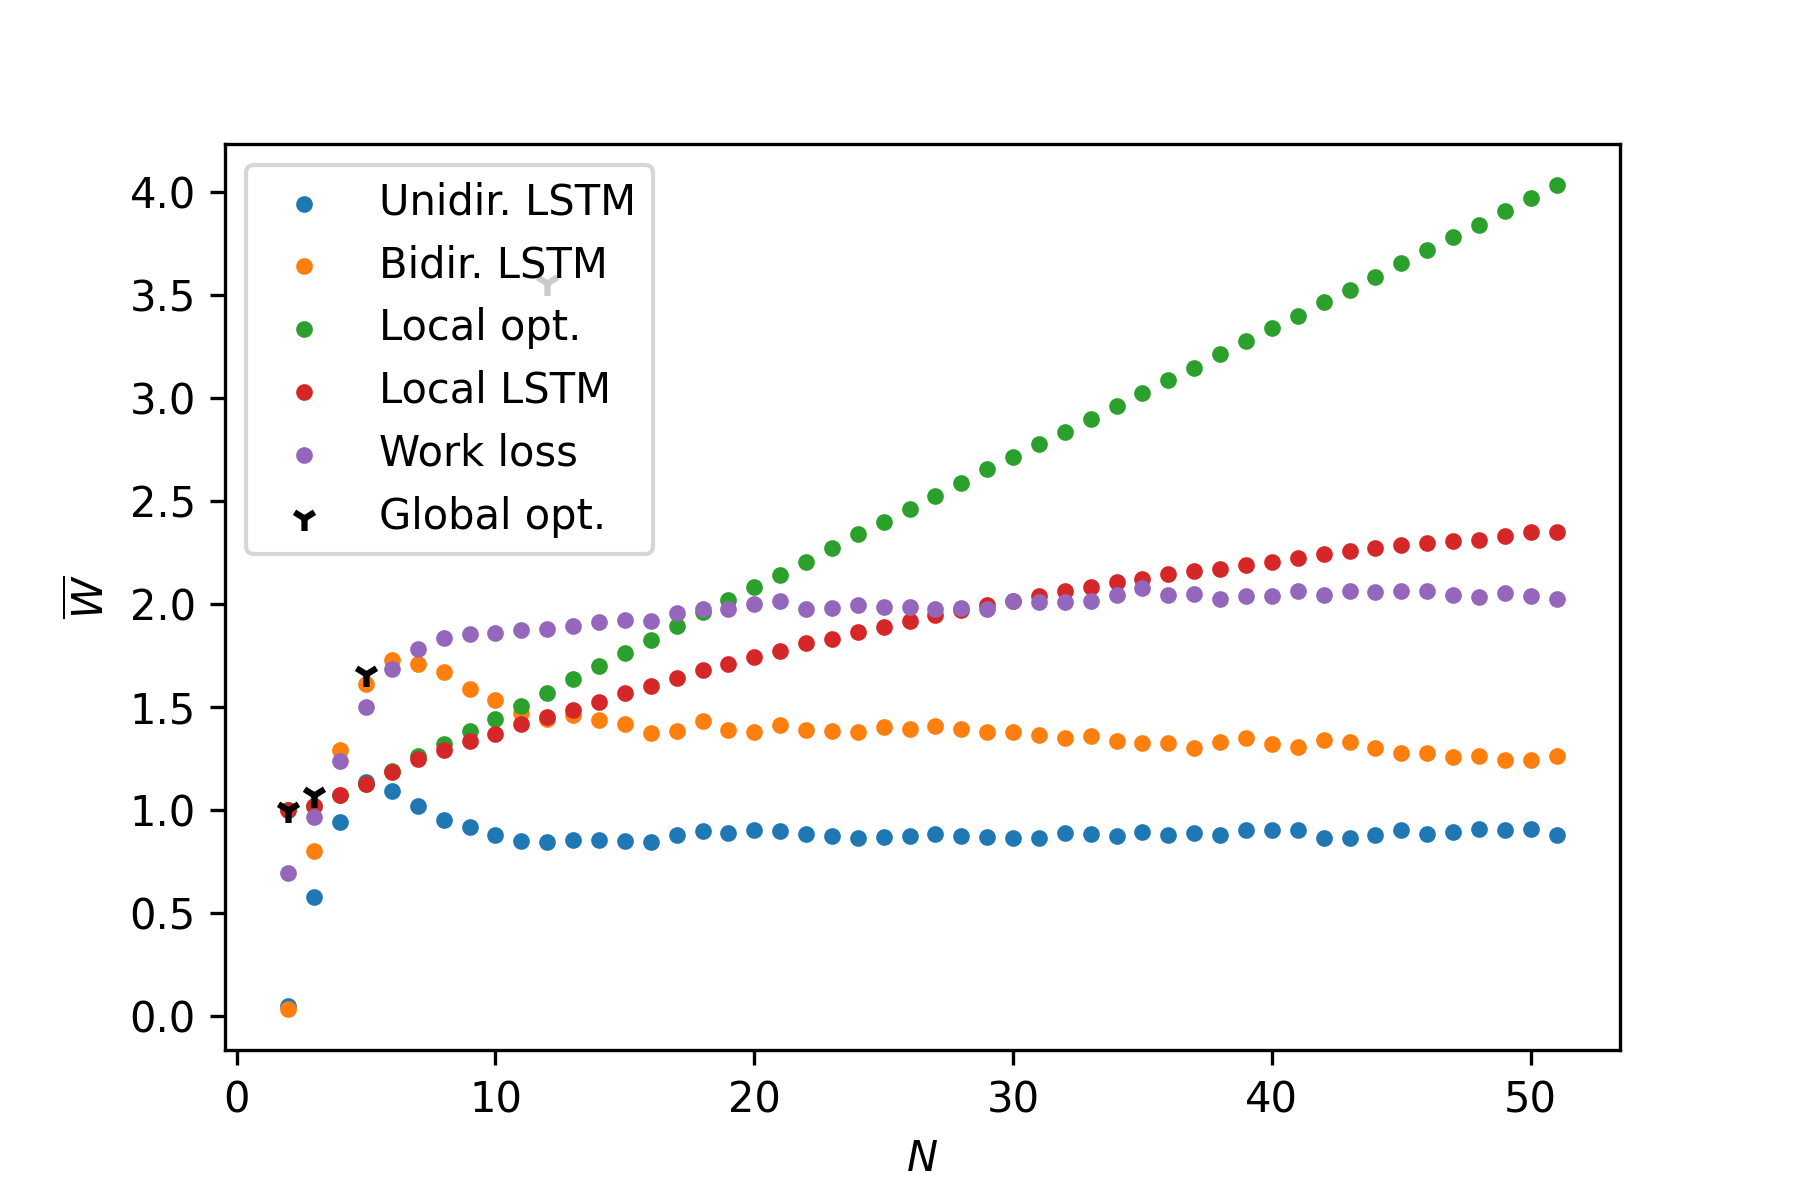
\includegraphics[width=\textwidth]{img/gen_dt_1}
		\subcaption{$\Delta \mathrm{T} = 1$}
	\end{subfigure}
	\begin{subfigure}{0.48\textwidth}
		\centering
		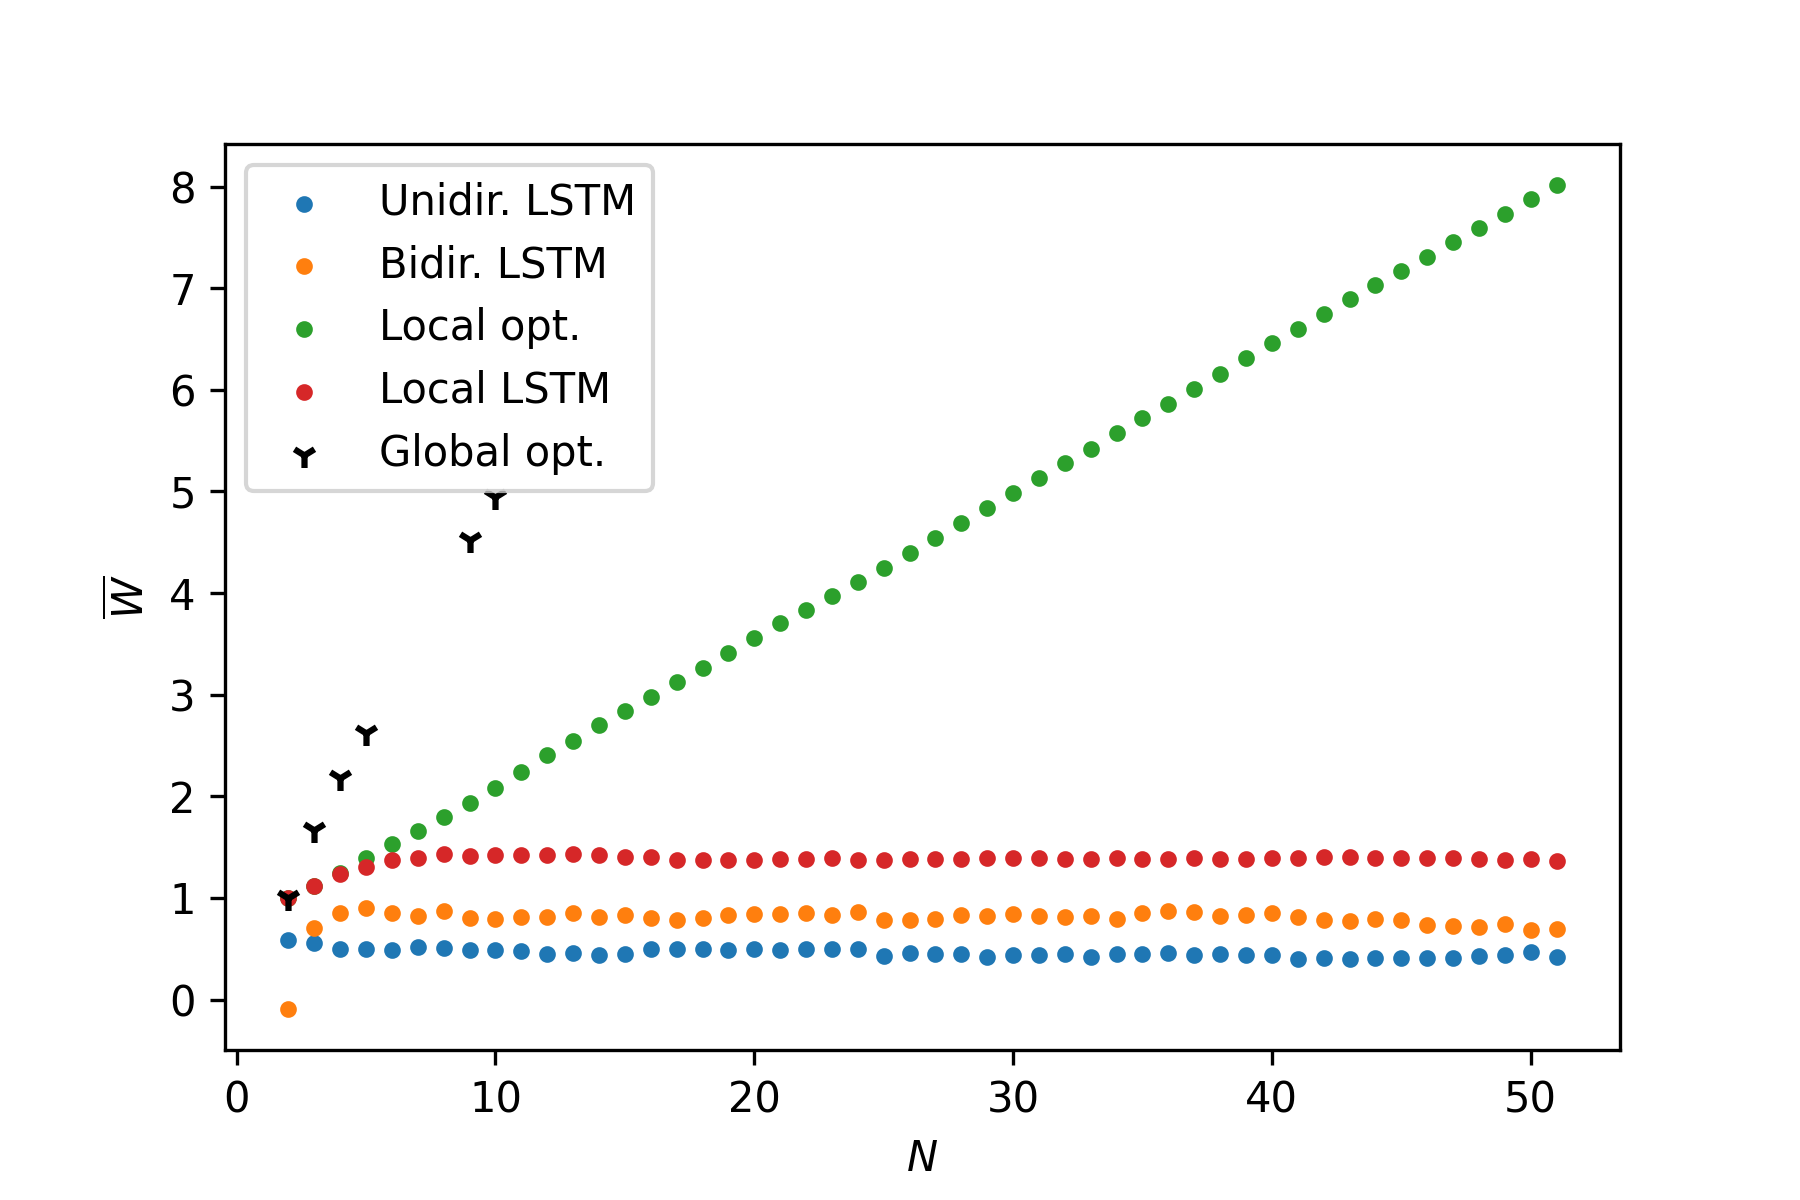
\includegraphics[width=\textwidth]{img/gen_dt_5}
		\subcaption{$\Delta \mathrm{T} = 5$}
	\end{subfigure}
	\caption{Generalisability of MSE and local optimisation models. For each $N$, we generate 1000 random drives and predict their transducer policies. We plot the mean of their work output $\overline{W}$ for varying $N$. Where available, we plot the optimal average work output. For $\Delta \mathrm{T} = 1$, we additionally plot $\overline{W}$ for the bidirectional LSTM trained using the extracted work as the loss function. The average output of the local optimisation protocol is plotted as a benchmark.}
	\label{genplot}
\end{figure}

For $\Delta \mathrm{T} = 5$, all models fail to generalise to larger $N$.
A possible reason can be found in the poor performance of the unidirectional LSTM trained on the locally optimised protocol.
Here, it becomes evident that the model is unable to learn a precise representation of the system state which remains valid for larger $N$.
Two possible reasons come to mind, firstly the larger evolution time leads to a faster propagation of errors in the representation.
Additionally, the mapping $U = e^{-i H_s \Delta \mathrm{T}}$ from initial to evolved state, which depends non-linearly on $\Delta \mathrm{T}$ and the model inputs and outputs, is more difficult to represent for the LSTM cell.
The quality of any polynomial approximation of $U$ learned by the model will degrade more quickly for large $\Delta \mathrm{T}$. 

\chapter{Conclusion and outlook}\label{outlook}
% !TeX root = ../BA_main_englisch.tex
% !TeX spellcheck = en_GB
We demonstrated that our approach is capable of predicting transducer policies that will produce a positive work output given a drive data set.
We found that the efficiency greatly depends on the model parameters $N$ and $\Delta \mathrm{T}$.
For $N=2$ and $\rho_0 = \ket{+}\bra{+}$, where an analytic optimum exists, a simple linear network is able to reproduce the optimal policy.
For the higher-dimensional case $N=5$, we examined two switching times $\Delta \mathrm{T}$, finding that the network performs better on the shorter than the longer time.


In all cases the bidirectional outperforms the unidirectional LSTM, as the former has access to the complete drive sequence while the latter can only make predictions from the previous and current drive qubits.

For $N=5$ and $\Delta \mathrm{T}=1$, ev
We identified the use of the mean squared error as a disadvantage in calculating the loss during training.
Training the network directly on the extracted work did not create models with greater predictive powers due to the non-convexity of the cost function.
Instead, following an approach similar to those in \cite{Banchi_2018, PhysRevX.10.011006}, where recurrent neural networks are used to directly model the system dynamics, might alleviate these shortcomings.

An extension to the model is to add dissipative effects to the system state $\rho_S$.

\bibliographystyle{unsrt}
\bibliography{biblio}

\appendix
\chapter{Derivations}
\section{Single extraction step work output}
\begin{align*}
	H_S(\theta_D^t, \phi_D^t, \theta_T^t, \phi_T^t) & = \frac{1}{2} \left[\sin(\theta_D^t) e^{i\phi_D^t} + \sin(\theta_T^t) e^{i\phi_T^t}\right] \sigma_{+} + h.c. \\
	& = \alpha \sigma_{+} + h.c. \\
\end{align*}
\begin{align*}
	dH & = H_S(\theta_D^t, \phi_D^t, \theta_T^{t+1}, \phi_T^{t+1}) - H_S(\theta_D^t, \phi_D^t, \theta_T^t, \phi_T^t) \\
	& = \frac{1}{2}(\sin(\theta_T^{t+1})e^{i\phi_T^{t+1}} - \sin(\theta_T^t)e^{i\phi_T^t}) \sigma_{+} + h.c. =: (\tau' - \tau) \sigma_{+} + h.c. \\
\end{align*}
\begin{align*}
	U & = e^{-iH_S \Delta \mathrm{T}} = 
	\exp \begin{pmatrix}
	0 & -i\alpha^* \Delta \mathrm{T} \\
	-i \alpha \Delta \mathrm{T} & 0 \\
	\end{pmatrix}\\
	& = 
	\frac{1}{2} \begin{pmatrix}
	\frac{\alpha^*}{\abs{\alpha}} & -\frac{\alpha^*}{\abs{\alpha}} \\
	1 & 1 \\
	\end{pmatrix}
	\begin{pmatrix}
	e^{-i\abs{\alpha} \Delta \mathrm{T}} & 0 \\
	0 & e^{i\abs{\alpha} \Delta \mathrm{T}} \\
	\end{pmatrix}
	\begin{pmatrix}
	\frac{\abs{\alpha}}{\alpha^*} & 1 \\
	-\frac{\abs{\alpha}}{\alpha^*} & 1 \\
	\end{pmatrix} \\
	& = \begin{pmatrix}
	\cos(\abs{\alpha}\Delta \mathrm{T}) & -i\frac{\alpha^*}{\abs{\alpha}} \sin(\abs{\alpha}\Delta \mathrm{T}) \\
	-i\frac{\abs{\alpha}}{\alpha^*} \sin(\abs{\alpha}\Delta \mathrm{T}) & \cos(\abs{\alpha} \Delta \mathrm{T}) \\
	\end{pmatrix} \\
\end{align*}
	With $\ket{\psi_0} = a \ket{0} + b \ket{1}$,  $\abs{a}^2 + \abs{b}^2 = 1$, we  have
\begin{align*}
	\rho_0 & = \begin{pmatrix}
	\abs{a}^2 & a b ^* \\
	a^* b & \abs{b}^2 \\
	\end{pmatrix}, \ \rho = U \rho_0 U^\dagger = 
	\begin{pmatrix}
	\rho_{00} & \rho_{01} \\
	\rho_{10} & \rho_{11} \\
	\end{pmatrix}  \\
	\rho_{00} & = \abs{a}^2 \ \cos^2(\abs{\alpha} \Delta \mathrm{T}) + \abs{b}^2 \ \sin^2(\abs{\alpha} \Delta \mathrm{T}) - \frac{1}{\abs{\alpha}} \sin(2 \abs{\alpha} \Delta \mathrm{T}) \Im{a b^* \alpha} \\
	\rho_{01} & = \frac{\alpha^*}{2 \abs{\alpha}} i \ \sin(2 \abs{\alpha} \Delta \mathrm{T}) (\abs{a}^2 - \abs{b}^2) + \frac{\alpha^*}{\alpha} a^* b \sin^2(\abs{\alpha} \Delta \mathrm{T}) + a b^* \ \cos^2(\abs{\alpha} \Delta \mathrm{T}) \\
	\rho_{10} & = 	\frac{\abs{\alpha}}{2 \alpha^*} i \ \sin(2 \abs{\alpha} \Delta \mathrm{T}) (\abs{b}^2 - \abs{a}^2) + \frac{\alpha}{\alpha^*} a b^* \ \sin^2(\abs{\alpha} \Delta \mathrm{T}) + a^* b \ \cos^2(\abs{\alpha} \Delta \mathrm{T}) \\
	\rho_{11} & = \abs{a}^2 \ \sin^2(\abs{\alpha} \Delta \mathrm{T}) + \abs{b}^2 \ \cos^2(\abs{\alpha} \Delta \mathrm{T}) + \frac{1}{\abs{\alpha}} \sin(2 \abs{\alpha} \Delta \mathrm{T}) \Im{a b^* \alpha}
\end{align*}
\begin{align*}
	\mathrm{dW} = & - \mathrm{Tr} \ \rho \ \mathrm{dH} = \frac{\abs{a}^2 - \abs{b}^2}{\abs{\alpha}} \sin(2 \abs{\alpha} \Delta \mathrm{T}) \Im{(\tau' - \tau) \alpha^*} \\
	& - 2 \ [\cos^2(\abs{\alpha} \Delta \mathrm{T}) \Re{(\tau' - \tau) a b^*} 
	+ \sin^2(\abs{\alpha} \Delta \mathrm{T}) \Re{(\tau' - \tau)a^* b \frac{\alpha^*}{\alpha}} ]
\end{align*} \label{deriv_jump}

\section{Optimal policy for $N=2$} \label{n2_opt_pol}
For $\rho_0 = \ket{+} \bra{+}$, or $a = e^{-i \phi_D}/\sqrt{2}, b = 1/\sqrt{2}$ following the notation used in appendix \ref{deriv_jump}, finding the optimal solution of $\mathrm{dW}$ for $N = 2$ requires finding the transducer setting that ensures
\begin{align}\label{commutator}
	[H_{DS}, H_S] = [\delta \sigma_{+} + \delta^* \sigma_{-}, \alpha \sigma_{+} + \alpha^* \sigma_{-}] = 0
\end{align}
with $\delta = \frac{1}{2} \sin{\theta_D} e^{i \phi_D}$.
\ref{commutator} is equivalent to
\begin{align*}
	\Im{\alpha \delta^*} = 0 \implies \arg{\alpha} = \phi_D \implies a b^* = a^* b \frac{\alpha^*}{\alpha},
\end{align*}
which leads to the independence of dW with regard to $\Delta \mathrm{T}$. 
\chapter{Training protocols}\label{training}
% !TeX spellcheck = en_GB
In all models we split the data into training, validation and test data with $p_{test} = 18 \%$ and $p_{valid} = 8.2 \%$. 
The models are implemented using the PyTorch library \cite{NEURIPS2019_9015}. 
Training is performed over $n$ epochs, in each of which the complete training set is used once in batches of \textit{batch size}.
In each batch, the gradient of the loss function with regard to the model parameters is calculated.
The gradient average over the data points in a batch are used to update the trainable parameters.
We use early stopping to stop training when the value of the cost function on the validation set does not improve for \textit{patience} epochs.
We apply dropout \cite{hinton2012improving} after all layers except for input and output.

\section{Hyperparameters Section \ref{n_2_ml}}
For $N=2$, we use the Adam optimiser with $\beta_1 = 0.9$, $\beta_2 = 0.98$ and $\epsilon = 10^{-9}$. The learning rate (LR) is determined by an exponential decay schedule
\begin{equation} \label{eds}
\mathrm{LR} \ (i) = \mathrm{initial \ LR} * \mathrm{decay \ rate}^i,
\end{equation}
where $i$ denotes the optimiser step.


\begin{table}[h]
	\centering
	\begin{tabular}{c | c | c }
		Patience & Initial LR & Decay Rate \\
		\hline
		100 & $10^{-2}$ & 0.995 \\
	\end{tabular}
	\caption{Hyperparameters used in training for the models in section \ref{n_2_ml}.}
	\label{hyperparams_n_2}
\end{table}

\section{Hyperparameters Sections \ref{n_5_ml} and \ref{n_5_dt1}}
The learning rate (LR) is determined by the `Reduce LR on Plateau' schedule.
The learning rate is multiplied by the hyperparameter \textit{factor} when the cost function does not improve for \textit{patience} / \textit{pat drop} epochs.
The hyperparameters are found using Bayesian optimisation implemented by \cite{wandb} and can be found in Table \ref{hyperparams_n_5}.
The FCANN in Section \ref{n_5_ml} has three hidden layers with 2000 neurons each.

\begin{table}[h]
	\centering
	\begin{tabular}{l | l}
		Hyperparameter & Value \\
		\hline
		Optimiser & SGD \\
		Batch size & 44 \\
		Dropout & 0.3179732914255167 \\
		Input layer 1 size & 793 \\
		Input layer 2 size & 488 \\
		Output layer size & 228 \\
		LSTM hidden size & 324 \\
		Large hidden size in Section \ref{n_5_dt1} & 552 \\
		Initial learning rate & 0.02847560288866327 \\
		LSTM layers & 3 \\
		Pat drop & 3.698498258242224 \\
		Patience & 55 \\
		Factor & 0.24509238889070978
	\end{tabular}
	\caption{Hyperparameters used for the models in Sections \ref{n5} and \ref{work_cost}.}
	\label{hyperparams_n_5}
\end{table}

% Erklärung
\clearpage
\thispagestyle{empty}
\minisec{Erklärung}\vspace*{1.5em}

Hiermit erkläre ich, dass ich diese Arbeit im Rahmen der Betreuung am Institut
für Theoretische Physik ohne unzulässige Hilfe Dritter verfasst und alle Quellen als solche gekennzeichnet habe.

\vspace*{45em}

Felix Soest \par
Dresden, Februar 2021

\end{document}
